\documentclass[english]{article}
\usepackage[title={Advanced Computer Architectures}, date={2022/2023}]{notestemplate}
\usepackage[external]{includetikz}

\title{Advanced Computer Architecture}
\begin{document}

\makecover
\clearpage
\chapter{Introduction to Computer Architectures}
\section{Introduction to Computer Architectures}
\subsection{MIPS Pipeline}
The MIPS Pipeline is a 5 stages micro processor that can be rappresented by this image:
\begin{figure}[h!]
    \centering
    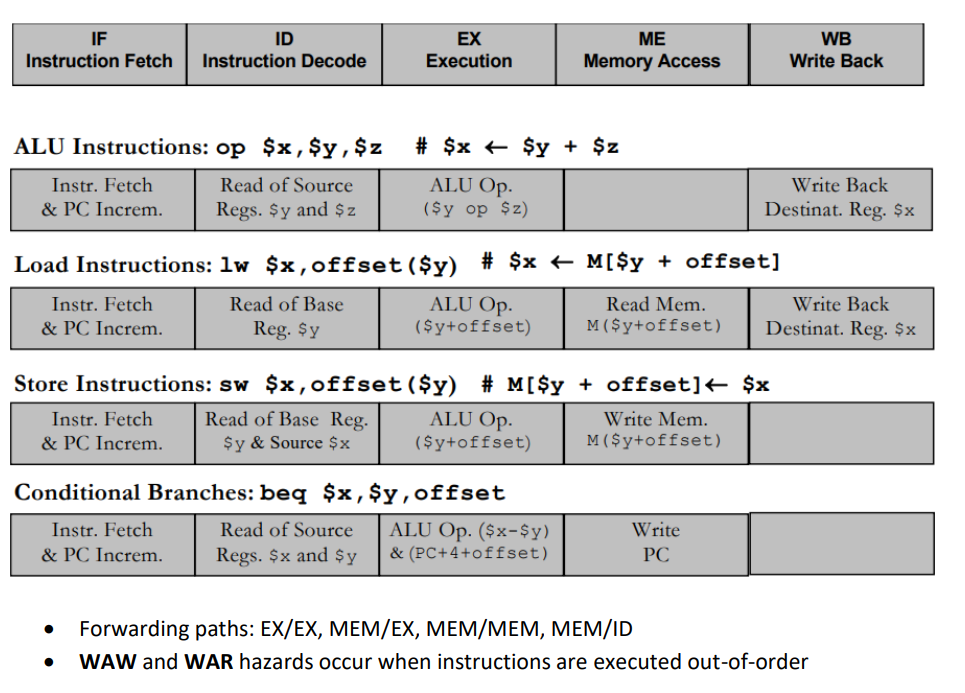
\includegraphics[scale=0.8]{Images/MIPS.png}
    \caption{This rappresent the 5 stages and the execution of the different type of operation}
    \label{fig:mips}
\end{figure}
\subsubsection{Optimization of MIPS Pipeline}
The most important optimization that an MIPS Processor can have are:
\begin{itemize}
    \item Forwarding path (Already wrote in \ref{fig:mips})
    \item Register File that can be read and wrote in the same clock cycle.
    \item Branch prediction (Will be explained later)
\end{itemize}
\subsubsection{Stages in \textit{MIPS} pipeline}

The \(5\) stages in the \textit{MIPS} pipeline are:

\begin{enumerate}
  \item \textbf{Fetch} - \texttt{IF}
        \begin{itemize}[label=\(\rightarrow\)]
          \item Instruction fetch from memory
        \end{itemize}
  \item \textbf{Decode} - \texttt{ID}
        \begin{itemize}[label=\(\rightarrow\)]
          \item Instruction decode and register read
        \end{itemize}
  \item \textbf{Execute} - \texttt{EX}
        \begin{itemize}[label=\(\rightarrow\)]
          \item Execute operation or calculate the address
        \end{itemize}
  \item \textbf{Memory access} - \texttt{ME}
        \begin{itemize}[label=\(\rightarrow\)]
          \item Access memory operand
        \end{itemize}
  \item \textbf{Write back} - \texttt{WB}
        \begin{itemize}[label=\(\rightarrow\)]
          \item Write the result back to register
        \end{itemize}
\end{enumerate}

Each instruction is executed after the previous one has completed its first stage, and so on.
When the pipeline is filled, five different activities are running at once.
Instructions are passed from one unit to the next through a storage buffer.
As each instruction progresses through the pipeline, all the information needed by the stages downstream must be passed along.

The stages are usually represented in Figure~\ref{fig:mips-pipeline-stages}.

\begin{figure}[htbp]
  \bigskip
  \centering
  \tikzfig[1.5]{image-7.tikz}
  \caption{Stages in \textit{MIPS} pipelines}
  \label{fig:mips-pipeline-stages}
  \bigskip
\end{figure}

\subsection{Flynn Taxonomy}
\label{sec:flynn-taxonomy}

Created in \(1996\) and upgraded in \(1972\), it provides the first description of a computer.

\begin{itemize}
  \item \textit{SISD} - \textbf{single} instruction, \textbf{single} data
        \begin{itemize}
          \item \textbf{Sequential} programs
          \item \textbf{Serial} (non parallel) computer
          \item \textbf{Deterministic} execution
          \item Only \textbf{one instruction stream} is being executed at a time
        \end{itemize}
  \item \textit{MISD} - \textbf{multiple} instructions, \textbf{single} data
        \begin{itemize}
          \item Multiple processors working in \textbf{parallel} on the same data
          \item \textbf{Fail safe} due to high redundancy
          \item The same algorithm is programmed and implemented in different ways, so if one fails the other is still able to compute the result
          \item \textbf{No practical market configuration}
        \end{itemize}
  \item \textit{SIMD} - \textbf{single} instruction, \textbf{multiple} data
        \begin{itemize}
          \item Each processor receives \textbf{different data} and performs the \textbf{same operations} on it
          \item Used in fields where a single operation must be performed in many different pieces of information \textit{(like in image processing)}
          \item Each instructions is executed in \textbf{synchronous} way on the same data
          \item Best suited for specialized problems characterized by a high degree of regularity, such as graphics or images processing
          \item \textbf{Data level parallelism} \textit{(DLP)}
        \end{itemize}
  \item \textit{MIMD} - \textbf{multiple} instructions, \textbf{multiple} data
        \begin{itemize}
          \item \textbf{Array of processors} in parallel, each of them executing its instructions
          \item Execution can be \textbf{asynchronous} or \textbf{synchronous}, \textbf{deterministic} or \textbf{non-deterministic}
          \item The \textbf{most common} type of parallel computer
        \end{itemize}
\end{itemize}
\clearpage
\begin{figure}[htbp]
  \bigskip
  \centering
  \tikzfig[1]{image-1.tikz}
  \caption{Flynn Taxonomy}
  \label{fig:flynn-taxonomy}
  \bigskip
\end{figure}
\subsection{Hardware parallelism}

There are different types of hardware parallelisms:

\begin{itemize}
  \item \textbf{Instruction Level parallelism} - \textit{(ILP)}
        \begin{itemize}
          \item Exploits data level parallelism at modest level through \textbf{compiler techniques} such as pipelining and at medium levels using speculation
        \end{itemize}
  \item \textbf{Vector Architectures} and \textbf{Graphic Processor Units}
        \begin{itemize}
          \item Exploit data level parallelism by applying a single instruction to a \textbf{collection of data} in parallel
        \end{itemize}
  \item \textbf{Thread level parallelism} - \textit{(TLP)}
        \begin{itemize}
          \item Exploits either data level parallelism or task level parallelism in a coupled hardware model that allows \textbf{interaction among threads}
        \end{itemize}
  \item \textbf{Request level parallelism}
        \begin{itemize}
          \item Exploits parallelism among largely decoupled tasks specified by the programmer or the OS
        \end{itemize}
\end{itemize}

Nowadays, heterogeneous systems \textit{(systems that utilize more than one type of parallelism)} are commonly used among all commercial devices.
\subsection{Pipeline and Hazard}
The pipeline \textit{CPI} \textit{(clocks per instruction)} can be calculated taking account of:

\begin{itemize}
  \item \textbf{Ideal} pipeline \textit{CPI}
        \begin{itemize}
          \item measure of the maximum performance attainable by the implementation
        \end{itemize}
  \item \textbf{Structural stalls}
        \begin{itemize}
          \item due to the inability of the \textit{HW} to support this combination of instructions
          \item can be solved with more \textit{HW} resources
        \end{itemize}
  \item \textbf{Data hazards}
        \begin{itemize}
          \item the current instruction depends on the result of a prior instruction still in the pipeline
          \item can be solved with \textit{forwarding} or \textit{compiler scheduling}
        \end{itemize}
  \item \textbf{Control hazards}
        \begin{itemize}
          \item caused by delay between the \texttt{IF} and the decisions about changes in control flow \textit{(branches, jumps, executions)}
          \item can be solved with \textit{early evaluation, delayed branch, predictors}
        \end{itemize}
\end{itemize}
The main features of the pipeline are:
\begin{itemize}
  \item \textbf{Higher throughput} for the entire workload
  \item Pipeline rate is limited by the \textbf{slowest} pipeline stage
  \item Multiple tasks operate \textbf{simultaneously}
  \item It \textbf{exploits parallelism} among instructions
  \item Time needed to \textit{"fill"} and \textit{"empty"} the pipeline reduces speedup
\end{itemize}
\subsection{Pipeline hazards}
\label{sec:pipeline-hazards}

An \textbf{hazard} is a fault in a pipeline.
A hazard is created whenever there is a dependence between instructions that are close enough such that the overlap introduced by pipelining would change the order of access to the operands involved in said dependence.
It prevents the next instruction in the pipeline from executing during its designated clock cycle, reducing the performance from the ideal speedup.

There are \(3\) classes of hazards:
\begin{enumerate}
  \item \textbf{Structural} hazards, due to attempting to use the same resource from different instructions at the same time
  \item \textbf{Data} hazards \textit{stalls}, due to attempting to use a result before it is ready
        \begin{itemize}
          \item \textit{Read after write} - \textit{RAW}
                \begin{itemize}[label=\(\rightarrow\)]
                  \item the instruction tries to read a source register before it is written by a previous instruction
                  \item it's also called \textit{dependence} by compilers
                  \item caused by an actual need for communication
                \end{itemize}
          \item \textit{Write after read} - \textit{WAR}
                \begin{itemize}[label=\(\rightarrow\)]
                  \item the instruction tries to write a destination register before it is read by a previous instruction
                  \item it's also called \textit{anti dependence} by compilers
                  \item caused by the reuse of the same register for different purposes
                \end{itemize}
          \item \textit{Write after write} - \textit{WAW}
                \begin{itemize}[label=\(\rightarrow\)]
                  \item the instruction tries to write before it is written by a previous instruction
                  \item it's also called \textit{output dependence} by compilers
                  \item caused by the reuse of the same register for different purposes
                \end{itemize}
        \end{itemize}
  \item \textbf{Control} hazards \textit{stalls}, due to the request of deciding on the next instruction to execute before the condition itself is evaluated
\end{enumerate}

\bigskip
\textit{Data stalls may occur with instructions such as}:
\begin{itemize}
  \item \textit{RAW} stall:
        \begin{verbatim}
    r3 := (r1) op (r2)
    r5 := (r3) op (r4)  // r3 has not been written yet\end{verbatim}

  \item \textit{WAR} stall:
        \begin{verbatim}
    r3 := (r1) op (r2)
    r1 := (r4) op (r5)  // r1 has not been read yet \end{verbatim}
  \item \textit{WAW}  \textit{stall}:
        \begin{verbatim}
    r3 := (r1) op (r2)
    r3 := (r6) op (r7) // r3 has not been written yet \end{verbatim}
\end{itemize}

\subsubsection{Solutions to data hazards}

There are many ways in which data hazards can be solved, such as:

\begin{itemize}
  \item \textbf{Compilation} techniques
        \begin{itemize}
          \item \textbf{Insertion of \texttt{nop}} instructions
          \item \textbf{Instructions scheduling}
                \begin{itemize}
                  \item the compiler tries to avoid that correlating instructions are too close
                  \item it tries to insert independent instructions among correlated ones
                  \item when it can't, it inserts \texttt{nop} operations
                \end{itemize}
        \end{itemize}
  \item \textbf{Hardware} techniques
        \begin{itemize}
          \item \textbf{Insertion} on \textit{bubbles} or \textit{stalls} in the pipeline
          \item Data \textbf{forwarding} or bypassing
        \end{itemize}
\end{itemize}

Both the compilation and the hardware techniques will be analyzed in depth in Section~\ref{sec:strategies-to-support-ilp}.

\clearpage
\chapter{Performance and cost}
\section{Performance and cost}

There are multiple types \textit{(classes)} of computers, each with different needs:
the performance measurement is not the same for each of them.
\textit{Price, computing speed, power consumption} can be metrics to measure the performance of a computer.

Programming has become so complicated that it's not possible to balance all the constraints manually;
while the computational power has grown bigger than ever before, energy consumption is now a sensible constraint.

The computer engineering methodology is therefore described as:

\begin{figure}[htbp]
  \bigskip
  \centering
  \begin{minipage}[h]{0.495\textwidth}
    \centering
    \tikzfig[1]{image-2.tikz}
  \end{minipage}
  \begin{minipage}[h]{0.495\textwidth}
    \begin{enumerate}
      \item \label{enum:methodology-start} \textit{evaluate} system by bottlenecks
      \item \textit{simulate} new designs and organizations
      \item \textit{implement} next generation systems
      \item \textit{repeat}
    \end{enumerate}
  \end{minipage}
  \caption{Computer engineering methodology}
  \label{fig:computer-engineering-methodology}
  \bigskip
\end{figure}
The picked qualities may change according to the use case or the user themself,
but 2 metrics are normally used:

\begin{enumerate}
  \item \textbf{Elapsed time}
        \begin{itemize}
          \item \(\texttt{execution time} = \texttt{time end} - \texttt{time start}\)
          \item More relevant for system user
        \end{itemize}
  \item \textbf{Completion rate}
        \begin{itemize}
          \item \(\texttt{completion rate} = \texttt{number of jobs} \div \texttt{elapsed time}\)
          \item More relevant for the system designer
        \end{itemize}
\end{enumerate}
\subsection{Response time vs throughput}

Is it true that
\(\texttt{throughput} = {1} \div { \texttt{average response time}}\)?
The answer can be given only if it's clear if there's an overlap between core operations.

If there is, then \[ \texttt{throughput} > {1} \div {\texttt{average response time}} \]
With pipelining, \textbf{execution time} of a single instruction is \textbf{increased} while the \textbf{average throughput} is \textbf{decreased}.

\subsection{Factors affecting performance}

A few of the factors affecting the performance are:

\begin{itemize}
  \item Algorithm complexity and data sets
  \item Compiler
  \item Instructions set
  \item Available operations
  \item Operating systems
  \item Clock rate
  \item Memory system performance
  \item I/O system performance and overhead
        \begin{itemize}
          \item this it's the least optimizable factor, the main focus is then to optimize all the others
        \end{itemize}
\end{itemize}
The locution \textbf{\(X\) is \(n\) times faster than \(Y\)} can be expressed as:

\begin{gather*}
  \dfrac{ExTime\ (Y)}{ExTime\ (X)}  = \dfrac{Performance\ (X)}{Performance\ (Y)} = Speedup\ (X, Y) \\
  Performance(X) = \dfrac{1}{ExTime\ (x)}
\end{gather*}

So, in order to optimize a system, it's necessary to focus on common sense (a \textit{sadly} valuable quality).
While making a design trade-off one must favour the frequent case over the infrequent one.

\textit{For example}:
\begin{itemize}
  \item Instructions fetch and decode unit is used more frequently than the multiplier
        \begin{itemize}
          \item it makes sense to optimize \textbf{instructions fetch unit} first
        \end{itemize}
  \item If database server has \(50\) disks processor, storage dependability is more important than system dependability
        \begin{itemize}
          \item it makes sense to optimize \textbf{storage dependability} first
        \end{itemize}
\end{itemize}

\subsubsection{Amdahl's law}

As seen before, the speedup due to the enhancement \(E\) is:
\[ Speedup\ (E)  = \dfrac{ExTime\ w/o\ E}{ExTime\ w/\ E} = \dfrac{Performance\ w/\ E}{Performance\ w/o\ E} \]

Suppose that enhancement \(E\) accelerates a fraction \(F\) of the task by a factor \(S\) and the remainder of the task is unaffected.
Amdahl's law states that:
\begin{gather*}
  ExTime_{new} = ExTime_{old} \times \left[\left(1 - F\right) + \dfrac{F}{S}\right] \\
  Speedup = \dfrac{ExTime_{old}}{ExTime_{new}} = \dfrac{1}{(1 - F) + \sfrac{F}{S}} = \dfrac{S}{S - SF + F}
\end{gather*}
\subsubsection{\textit{CPU} time}

\textbf{CPU time} is determined by:

\begin{itemize}
  \item \textbf{Instruction Count} - \textit{IC}:
        \begin{itemize}
          \item The number of executed instructions, not the size of static code
          \item Determined by multiple \textit{factors, including algorithm, compiler, ISA}
        \end{itemize}
  \item \textbf{Cycles per instructions} - \textit{CPI}:
        \begin{itemize}
          \item Determined by \textit{ISA} and \textit{CPU} organization
          \item Overlap among instructions reduces this term
          \item The \textit{CPI} relative to a process \texttt{P} is calculated as:
                \[ CPI(P) = \dfrac{\texttt{\# of clock cycles to execute P}}{\texttt{number of instructions}} \]
        \end{itemize}
  \item \textbf{Time per cycle} - \textit{TC}:
        \begin{itemize}
          \item It's determined by technology, organization and circuit design
        \end{itemize}
\end{itemize}

\bigskip
Then, \textit{CPU} time can be calculated as:
\[ CPU_{time} = T_{clock} \cdot CPI \cdot N_{inst} = \dfrac{CPI \cdot N_{inst}}{f} \]
Note that the \textit{CPI} can vary among instructions because each step of the pipeline might take different amounts of time.
The factors that can influence the \textit{CPU} time are shown in Table~\ref{tab:relation-factor-CPU-time}.

\begin{table}[htbp]
  \centering
  \begin{tabular}{r|c|c|c}
                             & \textit{IC} & \textit{CPI} & \textit{TC} \\ \hline
    \textit{Program}         & \xmark      &              &             \\
    \textit{Compiler}        & \xmark      & (\xmark)     &             \\
    \textit{Instruction set} & \xmark      & \xmark       &             \\
    \textit{Organization}    &             & \xmark       & \xmark      \\
    \textit{Technology}      &             &              & \xmark      \\
  \end{tabular}
  \caption{Relation between factors and \textit{CPU} time}
  \label{tab:relation-factor-CPU-time}
\end{table}
\subsubsection{Other metrics}

There are other metrics to measure the performance of a \textit{CPU}:

\begin{itemize}
  \item \textit{MIPS} - millions of instructions per second
        \[ MIPS = \dfrac{\texttt{number of instructions}}{\texttt{execution time} \cdot 10^6} = \dfrac{\texttt{clock frequency}}{\texttt{CPI} \cdot 10^6} \]
        \begin{itemize}
          \item the higher the \textit{MIPS}, the faster the machine
        \end{itemize}
  \item \textit{Execution time}
        \[ T_{execution} = \dfrac{\texttt{instruction count}}{\texttt{MIPS} \cdot 10^6} \]
  \item \textit{MFLOPS} - floating point operations in program
        \begin{itemize}
          \item assumes that floating points operations are independent of the compiler and ISA
          \item it's not always safe, because of:
                \begin{itemize}
                  \item missing instructions \textit{(e.g. FP divide, square root, sin, cos, \dots)}
                  \item optimizing compilers
                \end{itemize}
        \end{itemize}
\end{itemize}
\clearpage
\chapter{Cache}
\section{Cache Memories}
In computing, a cache is a hardware or software component that stores data so that future request for that data can be server faster.
The data stored in a cache might be the result of an earlier computation or a copy of data that are stored elsewhere.
\subsection{Why use cache?}
The reasone that why we use cache is because we need to improve performance of memory, because the time access of it is always slower than CPU's clock cycle.
So our goal is:
\begin{itemize}
    \item Provide the user the illusion to use a memory that is fast and large at the same time.
    \item Provide the data to processor at high frequency.
\end{itemize}
\subsection{How a cache is made?}
A cache i made up of block, that is a fixed-size colloction of data containg the requested word.\\
The number of \textit{Cache blocks} is calculated from \textit{Cache Size} and \textit{Block Size} by the following formula:
\begin{equation*}
    \textit{Number Of Blocks } = \frac{Cache Size}{Block Size}
\end{equation*}
To understand how a cache works we need to introduce two crucial thing
\begin{itemize}
    \item \textit{Temporal Locality}, it's tells us that we are likely to need this word again in near future.
    \item \textit{Spatial Locality}, rappresent the trend that if we need to use a memory space there is an high probability that we need again an near memory space.
\end{itemize}
The cache exploits both types of predictability.
\subsection{Definition of cache}
If we need to use a cache we need to know some terminology.
\begin{itemize}
    \item \textbf{Hit Rate}, is the number of memory access that find the data in the upper level\footnote{There are a lot of level of memory, also in cache} with respect to the total number of memory accesses.
    \begin{equation*}
        Hit Rate = \frac{#Hits}{#MemoryAccess}
    \end{equation*}
    \item \textbf{Hit Time}, time to access the data in the upper level of the hierarchy, including the time nedeed to understand if the attempt is and hit or a miss.
    \item \textbf{Miss Rate}, number of memory access that don't find the data in the upper level.\footnote{The sum of $ Miss Rate + Hit Rate = 1$ must be this}
    \begin{equation*}
        Miss Rate = \frac{#Miss}{#MemoryAccess}
    \end{equation*}
    \item \textbf{Miss Penalty}, time needed to access the lower level and to replace the block in the upper level, with this date we can calculate \textbf{\textit{Miss Time}} by this formula:
    \begin{equation*}
        Miss Time = Hit Time + Miss Penalty
    \end{equation*}
    \item \textbf{Average Memory Access Time} \textit{AMAT}, is described by this formula.
    \begin{equation*}
        AMAT = Hit Time + Miss Rate\cdot MissPenalty
    \end{equation*}
\end{itemize}
\subsection{Cache Structure}
Eache entry in the cache must follow a structure that is:
\begin{itemize}
    \item \textbf{Valid bit }indicate if the position contains valid data.
    \item \textbf{Cache tag} containts the value that univocally identifies the memory addres corrisponding to the stored data.
    \item \textbf{Cache Data} containt the data.\footnote{grazie al cazzo}
\end{itemize}
In cache the most common problem is the block placement, because we need to find the corrispondence between the memory address of the block and the cache address of the block, there are 3 principal types:
\begin{itemize}
    \item Direct Mapped, means that each memory location corresponds to one and only one cache location.\\
    The cache address of the block is given by to bigger block:
    \begin{itemize}
        \item Block address, that contains tag and index
        \item Block offeset, that contains word offset and byte offset
    \end{itemize}
    \item Fully Associative, the memory block can be placed in any position of the cache, the index doesn't exist in the memory address.
    \item N-Way Set Associative, the cach is composed of sets each set composed of $n$ blocks, the sets are calculated by the following formula:
    \begin{equation*}
        NumberOfSets = \frac{CacheSize}{BlockSize\cdot N}
    \end{equation*}
    \begin{figure}[h!]
    \centering
    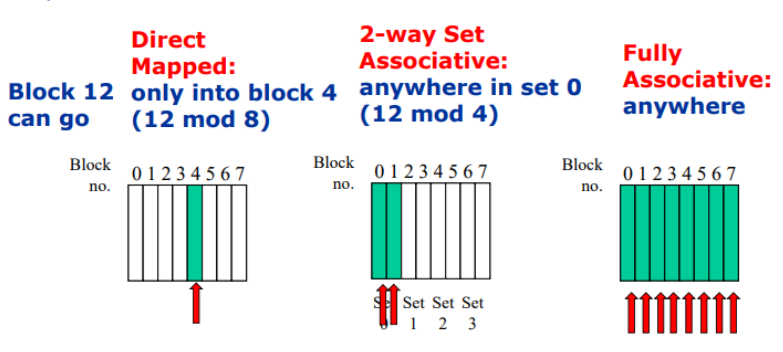
\includegraphics[scale=0.8]{Images/cache.png}
    \caption{Recap of cache memory}
    \label{fig:mips}
\end{figure}
\end{itemize}
\clearpage
\subsection{How to improve Cache?}
The increment of cache throughput or a hit rate is an important job in CPU development.\\
\subsubsection{Increment of associativity}
This type of improvement will reduce the miss rate, but is a double sword\footnote{Lama a doppio taglio? Non lo so sono mezzo analfabeta} brings a higher cost and increment of hit time caused by the bigger number of sets.
\subsubsection{Block Replacement}
In case of a miss in a \textit{Fully associative cache}, we need to decide which block to replace, in \textit{set-associative}, we need to select among the blocks of the selected set, meanwhile, in \textit{a direct mapped cache}, we must replace the selected one.\\
For every type of cache, except for directly mapped, we need to create strategies to change, there are three principal types:
\begin{itemize}
    \item Random
    \item Least Recently Used
    \item FIFO
\end{itemize}
But the choosing strategy is not enough for a sufficient fix, we need a \textit{\textbf{Write Policy}}
\subsection{Write Policy}
This policy defines how to write in a selected block.
\subsubsection{Write-Through}
The information is written to both the block in the cache and the block in the lower level
\subsubsection{Write-Back}
The information is written \textbf{\textit{only}} to the block in the cache, with this policy we need to introduce a \textbf{Dirty bit}
\subsubsection{Main Difference}
The main difference between these two policies can be reassumed in this simple scheme:
\begin{itemize}
    \item Write Back:
\begin{itemize}
        \item The block can be written by the processor at the frequency at which the cache, and not the main memory can accept it 
        \item Multiple writes to the same block require only a single write to the main memory
    \end{itemize}
    \item Write Through:
\begin{itemize}
    \item Simpler to be implemented, but it needs to create a \textit{Write buffer} (\ref{sec:writeBuffer})
    \item The read miss is cheaper because they do not require any writing to lower level
    \item The memory is always up to date
\end{itemize}
\end{itemize}
\subsubsection{Write Buffer}\label{sec:writeBuffer}
Insert a \textbf{FIFO buffer} to not wait for lower-level memory access, so in this way, the processor writes data to the cache and writes buffer, and the memory controller will write all the content into the main memory. There's still a problem, the saturation of this buffer.
\subsection{Write Miss Option}
This option explains what to do if a write miss occurs.
\subsubsection{Write Allocate}
Allocate a new cache line in the cache then write, is a double write to cache, which usually means that you must do a "read miss" to fill in the rest of the cache line.\\
Usually is used with \textit{a Write-Back} policy
\subsubsection{No-Write allocate}
Simply send write data to lower-level memory, and don't allocate a new line.\\
Usually is used with \textit{Write-Through} policy
\subsection{Memory Hierarchy}
The goal of a CPU developer is to give the illusion of unlimited amounts of memory with low latency, but fast memory(\textit{SRAM}) cost a lot with respect to cheaper and slower like \textit{DRAM}.\\
To jump out of this problem we organize the memory system into a hierarchy, with \textit{Temporal and Spatial Locality} we can ensure that nearly all references can be found in the smaller memories, reaching our goal.
\subsection{Classification of Cache Miss}
The cache miss could be categorized into three major types:
\begin{itemize}
    \item Compulsory Misses, the first access to a block that is not in the cache, is also called \textit{\textbf{Cold Start.}}
    \item Capacity Misses, if the cache cannot contain all the blocks needed during the execution of a program, capacity misses will occur due to blocks being replaced and later retrieved.
    \item Conflict Misses can occur only in set-associative or direct mapped, this occurs because a block can be replaced and later retrieved when other blocks map to the same location in the cache.
\end{itemize}\clearpage
\section{Improve cache performance}
There are three ways to improve the cache performance, and all of these refer to a reduction of something in the \textit{\textbf{AMAT} } calculation.
\subsection{Reducing the miss rate}
There are different ways to reduce the miss rate:
\begin{enumerate}
    \item Increase the cache capacity, but this brings an increase in cost, hit time, and power consumption.
    \item Increasing the block size, this increase misses penalty and conflict misses if the cache is small.
    \item Higher Associativity, this increase hit time, area, power consumption, and cost.\\
Is possible to use the \textit{\textbf{MultiBanked caches}}, this type of cache introduces a sort of associativity, by organizing the cache as independent banks to support simultaneous access to increase the cache bandwidth.
\item Victim Cache is a small fully associative cache used as a buffer to place data discarded from the cache to better exploit temporal locality, is placed between the cache and its refilling path. Is checked on a miss to see if it has the required data before going to lower-level memory, if the block is found the victim block and the cache block are swapped.
\item Pseudo-Associativity and Way Prediction:
    \begin{itemize}
        \item Way prediction uses extra bits to predict for each set which of the n-ways\footnote{Si USA solo nei n-way set-associative} to try on the next cache access.
        \item Pseudo-associativity\footnote{Questo solo in direct mapped} divides the cache into two banks in a sort of associativity.
    \end{itemize}
    \item Hardware Pre-Fetching of instruction and data, to exploit locality pre-fetch next instruction before they are requested by the processor, this solution relies on extra memory bandwidth that can be used without penalty. But if pre-fetching interferes with demand misses it can lower performance.
    \item Software Pre-Fetching data, compiler inserts prefetch \textit{LOAD} instruction to load data in registers/cache before they are needed, this adds an overhead due to LOAD instruction.
    \item Compiler Optimizations, the idea is to apply profiling on SW application, the use profiling info to apply code transformation.
\begin{itemize}
    \item Reordering instruction to reduce conflict misses.
    \item Merging Arrays to improve spatial locality
    \item Loop Interchange to improve spatial locality by changing loops nesting access data in the order stored in memory
    \item Loop Fusion to improve spatial locality by combining two independent loops
    \item Loop Blocking improves temporal locality by accessing the "Sub-Block" of data repeatedly.
\end{itemize}
\end{enumerate}
\subsection{Reducing the miss penalty}
\begin{enumerate}
    \item Read Priority over Write on Miss, giving higher priority to reading misses overwrites to reduce the miss penalty, the write buffer must be properly sized. This approach can complicate memory access because the write buffer might hold the updated value of a memory location needed on a read miss.
\begin{itemize}
    \item Write Through with write buffers might generate \textit{RAW} conflicts with main memory read on cache misses, so we need to read the contents of the write buffer on a read miss if there are no conflicts we let the memory access continue sending the read miss before the write, otherwise, the read miss has to wait until the flush of the write buffer.
    \item Write Back, instead of writing the dirty block to memory we could copy the dirty block to a write buffer then do the read miss and after write to memory, this reduces CPU stalls.
\end{itemize}
\item Sub-Block placement, we move the sub-block instead of the full block. We need valid bits, but we can't exploit enough spatial locality.
\item Early Restart and Critical Word First, usually the CPU needs just one word of the block on a miss, so we don't wait for the full block to be loaded before restarting the CPU.
\begin{itemize}
    \item Early restart, request the words in normal order from memory, but as soon as the requested word of the block arrives, send it to the CPU to let it continue execution while filling the rest of the block.
    \item Critical Word First, request the missed word first from memory and send it to the CPU as soon as it arrives to let the CPU continue execution while filling the rest of the cache block.
\end{itemize}
These two technique is generally used only for large blocks and spatial locality tend to want the next sequential words.
\item Non-Blocking Cache allows the data cache to continue to supply cache hits during a previous miss.
\begin{itemize}
    \item Hit under Miss reduces the effective miss penalty by working during a miss instead of stalling CPU on misses, requires out-of-order execution CPU, and is a sort of out-of-order pipelined memory access.
    \item Hit  under Multiple Miss or Miss under Miss, may further lower the effective miss penalty overlapping multiple misses, requiring multiple memory banks to serve multiple misses. This increases the complexity of the cache controller.
\end{itemize}
\item Introduce a second-level Cache, large enough to capture many accesses that would go to main memory reducing the effective miss penalty.
\item Merging Write Buffer, each entry of the write buffer can merge words from  different memory addresses, trying to reduce stalls due to a full write buffer.
\end{enumerate}
\subsection{Reducing the hit time}
\begin{enumerate}
    \item Fast hit times via small and simple L1 Cache, direct mapped, small and simple on-chip L1 cache.
    \item Avoiding Address Translation, avoiding virtual address translation during indexing of cache, if the index is a physical part of the address can start tag access in parallel with address translation so that can compare to the physical tag.
    \item Pipelined writes, to pipeline tag check and update cache data as separate stages, the delayed write buffer must be checked on reads either complete write or read from write buffer.
    \item Small sub-blocks for write-through, if most write are 1-word, and sub-block are sized in 1-word write-through always write sub-block and tag immediately.
\begin{itemize}
    \item Tag Match and valid bit set, writing the block was proper, and nothing was lost by setting a valid bit on again.
    \item Tag Match and valid bit not set, writing data into the sub-block makes it appropriate to turn the valid bit on.
    \item Tag mismatch, this is a miss and will modify the data portion of the block. 
\end{itemize}
\end{enumerate}
\clearpage
\section{Pipeline}
\subsection{Complex in-order pipeline}

While using floating points operations, a few questions might arise:

\indentquote{What happens, architecture-wise, when mixing integer and floating point operations? How are different registers handled? How can \textit{GPRs (general purpose registers)} and \textit{FPRs (floating point registers)} be matched?}

\begin{figure}[htbp]
  \bigskip
  \centering
  \tikzfig[1]{image-8.tikz}
  \caption{Complex-in order pipeline}
  \label{fig:complex-in-order-pipeline}
  \bigskip
\end{figure}

In the complex in-order pipeline there isn't a single \textit{ALU} anymore but the execution of floating point operations is split between a number of \textit{Functional Units}.
The \textit{issue} stage detects conflicts while accessing any of them and it's able to delay the execution \textit{(by using stalls)} of instructions in case of errors.

The pipeline is now constituted by \(6\) stages, normally represented as in Figure~\ref{fig:mips-pipeline-stages-issue}.

\begin{figure}[htbp]
  \bigskip
  \centering
  \tikzfig[1.5]{image-9.tikz}
  \caption{Pipeline stages with issue}
  \label{fig:mips-pipeline-stages-issue}
  \bigskip
\end{figure}

Pipelining becomes complex when we want high performance in the presence of:

\begin{itemize}
  \item \textbf{Long latency} or partially pipelined floating point units
  \item \textbf{Multiple functions} and memory units
  \item Memory systems with \textbf{variable access time}
  \item Precise \textbf{exception}
\end{itemize}

Formally, all the different executions must be balanced.

\begin{figure}[htbp]
  \bigskip
  \centering
  \tikzfig[0.7]{image-10.tikz}
  \caption{Complex pipelining}
  \label{fig:complex-pipelining-2}
  \bigskip
\end{figure}

\bigskip
The main issues are found in:
\begin{itemize}
  \item \textbf{Structural conflicts at the execution stage} if some \textit{FPU} or memory unit is not pipelined and takes more than one cycle
  \item \textbf{Structural conflicts at the write-back stage} due to variable latencies of different Functional Units (or \textit{FUs})
  \item \textbf{Out of order write hazards} due to variable latencies of different \textit{FUs}
  \item Hard to handle exceptions
\end{itemize}

A possible technique to handle write hazards without equalizing all pipeline depths and without bypassing is by delaying all writebacks so all operations have the same latency into the \texttt{WB} stage.
In this approach, the following events will happen:

\begin{itemize}
  \item Write ports are \textbf{never oversubscribed}
        \begin{itemize}
          \item one instruction \textit{in} and one instruction \textit{out} for every cycle
        \end{itemize}
  \item Instruction commit happens \textbf{in order}
        \begin{itemize}
          \item it simplifies the precise exception implementation
        \end{itemize}
\end{itemize}

How is it possible to prevent increased write-back latency from slowing down single-cycle integer operations?
Is it possible to solve all write hazards without equalizing all pipeline depths and without bypassing them?

\subsection{Instructions issuing}
\label{sec:instructions-issuing}

To reach higher performance, more parallelism must be extracted from the program.
In other words, dependencies must be detected and solved, while instructions must be scheduled to achieve the highest parallelism of execution compatible with available resources.

A data structure keeping track of all the instructions in all the functional units is needed.
In order to work properly, it must make the following checks before the \texttt{issue} stage to dispatch an instruction:

\begin{enumerate}
  \item Check if the \textbf{functional unit} is available
  \item Check if the \textbf{input data} is available
        \begin{itemize}
          \item \textit{Failure in this step would cause a RAW}
        \end{itemize}
  \item Check if it's safe to write to the \textbf{destination}
        \begin{itemize}
          \item \textit{Failure in this step would cause a WAR or a WAW}
        \end{itemize}
  \item Check if there's a \textbf{structural conflict} at the \texttt{WB} stage
\end{enumerate}

Such a suitable data structure would look like in Table~\ref{tab:data-structure-keep-track-functional-units}.

\begin{table}
  \bigskip
  \centering
  \begin{tabular}{r|c|cccc}
    \hline
    \textit{name}   & \textit{busy} & \textit{op} & \textit{destination} & \textit{source 1} & \textit{source 2} \\ \hline
    \texttt{int}    &               &             &                      &                   &                   \\
    \texttt{mem}    &               &             &                      &                   &                   \\ \hline
    \texttt{add 1}  &               &             &                      &                   &                   \\
    \texttt{add 2}  &               &             &                      &                   &                   \\
    \texttt{add 3}  &               &             &                      &                   &                   \\ \hline
    \texttt{mult 1} &               &             &                      &                   &                   \\
    \texttt{mult 2} &               &             &                      &                   &                   \\ \hline
    \texttt{div}    &               &             &                      &                   &                   \\
  \end{tabular}
  \caption{Data structure to keep track of \textit{FUs}}
  \label{tab:data-structure-keep-track-functional-units}
  \bigskip
\end{table}

An instruction at the \texttt{issue} stage consults this table to check if:

\begin{itemize}
  \item The \textit{FU} is \textbf{available} by looking at the \textit{busy} column
  \item A \textit{RAW} can arise by looking at the \textit{destination} column for its \textbf{sources}
  \item A \textit{WAR} can arise by looking at the \textit{source} columns for its \textbf{destinations}
  \item A \textit{WAW} can arise by looking at the \textit{destination} columns for its \textbf{destinations}
\end{itemize}

When the checks are all completed:

\begin{itemize}
  \item An entry is \textbf{added} to the table if no hazard is detected
  \item An entry is \textbf{removed} from the table after \texttt{WB} stage
\end{itemize}

\bigskip
Later in the course \textit{(Section~\ref{par:CDC6600-scoreboard})}, this approach will be discussed more in-depth.

\subsection{Dependences}

Determining \textbf{dependences} among instructions is critical to defining the amount of parallelism existing in a program.
If two instructions are dependent, they cannot execute in parallel: they must be executed in order or only partially overlapped.

There exist \(3\) different types of dependences:

\begin{itemize}
  \item \textbf{Name} Dependences
  \item \textbf{Data} Dependences
  \item \textbf{Control} Dependences
\end{itemize}

While hazards are a property of the pipeline, dependences are a property of the program.
As a consequence, the presence of dependences does not imply the existence of hazards.

\subsubsection{Name Dependences}

\textbf{Name dependences} occurs when \(2\) instructions use the same register or memory location \textit{(called name)}, but there is no flow of data between the instructions associated with that \textit{name}.
Two types of name dependences could exist between an instruction \texttt{i} that precedes an instruction \texttt{j}:

\begin{itemize}
  \item \textbf{Antidependence}: when \texttt{j} writes a register or memory location that instruction \texttt{i} reads; the original instruction ordering must be preserved to ensure that \texttt{i} reads the correct value
  \item \textbf{Output Dependence}: when \texttt{i} and \texttt{j} write the same register or memory location; the ordering of the original instructions must be preserved to ensure that the value finally written corresponds to \texttt{j}
\end{itemize}

Name dependences are not true data dependences, since there is no value \textit{(no data flow)} being transmitted between instructions.
If the name \textit{(either register or memory location)} used in the instructions could be changed, the instructions do not conflict.

Dependences through memory locations are more difficult to detect (this is called the \inlinequote{memory disambiguation} problem), since two different addresses may refer to the same memory location.
As a consequence, it's easier to rename a \textbf{register} than rename a \textbf{memory location}.
It can be done either \textbf{statically} by the compiler or \textbf{dynamically} by the hardware.

\subsubsection{Data Dependences}

A data or name dependence can potentially generate a data hazard (\textit{RAW} for the former or \textit{WAR} and \textit{WAW} for the latter), but the actual hazard and the number of stalls to eliminate them are properties of the pipeline.

\subsubsection{Control Dependeces}

\textbf{Control dependences} determine the ordering of instructions.
They are preserved by two properties:

\begin{enumerate}
  \item \textbf{Instructions execution in the program order} to ensure that an instruction that occurs before a branch is executed at the right time \textit{(before the branch)}
  \item \textbf{Detection of control hazards} to ensure that an instruction \textit{(that is control dependent on a branch)} is not executed until the branch direction is known
\end{enumerate}

Although preserving control dependence is a simple way to preserve program order, control dependence is not the critical property that must be preserved.

\clearpage
\section{Branch Prediction}
The main goal of the \textbf{branch prediction} is to evaluate as early as possible the outcome of a branch instruction.
Its performance depends on:

\begin{itemize}
  \item The \textbf{accuracy}, measured in terms of the percentage of incorrect predictions given
  \item The \textbf{cost of an incorrect prediction} measured in terms of time lost to execute useless instructions \textit{(misprediction penalty)} given by the processor architecture
        \begin{itemize}
          \item the cost increases for deeply pipelined processors
        \end{itemize}
  \item \textbf{Branch frequency} given by the application
        \begin{itemize}
          \item the importance of accurate branch prediction is higher in programs with higher branch frequency
        \end{itemize}
\end{itemize}
There are many methods to deal with performance loss due to branch hazards:

\begin{itemize}
  \item \textbf{Static} branch prediction techniques: the actions for a branch are fixed for each branch during the entire execution
        \begin{itemize}
          \item used in processors where the expectation is that the branch behaviour is highly predictable at compile time
          \item can be used to assist dynamic predictors
        \end{itemize}
  \item \textbf{Dynamic} branch prediction techniques: the actions for a branch can change during the program execution
\end{itemize}

In both cases, care must be taken not to change the processor state until the branch is definitely known.
\subsection{Static techniques}
Usually it's done at compile time, because is used whene the target application has an highly predictiable  branch.
There are 5 commonly used branch prediction techniques:

\begin{itemize}
  \item Branch \textbf{always not taken}
  \item Branch \textbf{always taken}
  \item Backward \textbf{taken forward not taken}
  \item Profile \textbf{driven prediction}
  \item Delayed \textbf{branch}
\end{itemize}
	\subsubsection{Branch Always Not Taken}
	\label{sec:branch-always-not-taken}
	
	The branch is always assumed as \textbf{not taken}, thus the sequential instruction flow that has been fetched can continue as if the branch condition was not satisfied.
	If the condition in the state \texttt{ID} will result as not satisfied \textit{(and the prediction is correct)} performance can be preserved.
	
	If the condition in stage \texttt{ID} will result in satisfied \textit{(and the prediction is incorrect)} the branch is taken: the next instruction already fetched is flushed \textit{(turned into a \texttt{nop})} and the execution is restarted by fetching the instruction at the branch target address.
	There is a one-cycle penalty, so 4 nop.
 \begin{figure}[h!]
     \centering
     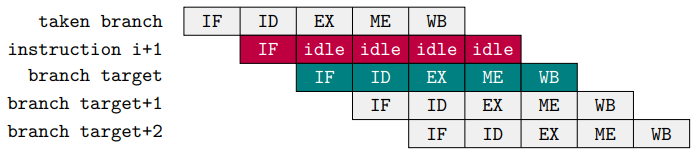
\includegraphics{Images/Screenshot 2023-05-16 121702.png}
     \caption{Rappresentation of missprediction}
     \label{fig:my_label}
 \end{figure}
\subsubsection{Branch Always Taken}
\label{sec:branch-always-taken}

An alternative scheme is to consider \textbf{every branch as taken}: as soon as the branch is decoded and the branch target address is computed, the branch is assumed to be taken and the fetching and the execution stages can begin at the target.

The predicted-taken scheme makes sense for pipelines where the branch target is known before the actual outcome.
This is not the case within \textit{MIPS} pipeline \textit{(where the branch target is known only after the operation outcome)}, so \textbf{there is no advantage in this approach}.
\subsubsection{Backward Taken Forward Not Taken}
\label{sec:backward-taken-forward-not-taken}

The prediction is based on the branch direction:

\begin{itemize}
  \item \textbf{Backward} going branches are predicted as \textbf{taken}
        \begin{itemize}
          \item the branches at the end of loops are likely to be executed most of the time
        \end{itemize}
  \item \textbf{Forward} going branches are predicted as \textbf{not taken}
        \begin{itemize}
          \item the \textbf{if} branches are likely not executed most of the time
        \end{itemize}
\end{itemize}
\subsubsection{Profile Driven Prediction}
\label{sec:profile-driven-prediction}

The branch prediction is based on profiling information collected from earlier runs.
This method can use compiler hints, and it's potentially more effective than the other ones;
however, it's also the most complicated between the \(5\) as it needs additional hardware.

This technique will be explored in Section~\ref{sec:dynamic-branch-prediction}.

\subsubsection{Delayed Branch}
\label{sec:delayed-branch}

The compiler statically schedules an independent instruction in the branch delay slot, which is then executed whether or not the branch is taken.

If the branch delay consists of one cycle (as in \textit{MIPS}), there's only one delay slot;
almost all processors with delayed branches have a single delay slot, as it's difficult for the compiler to fill more than one of them.

If the branch:

\begin{itemize}
  \item \textbf{Is untaken}: the execution continues with the instruction after the branch
  \item \textbf{Is taken}: the execution continues at the branch target
\end{itemize}
The compiler's job is to make the instruction placed in the branch delay slot valid and useful.
There are three ways in which the branch delay slot can be scheduled:

\begin{enumerate}
  \item From \textbf{before}
  \item From \textbf{target}
  \item From \textbf{fall through}
\end{enumerate}

These methods will be better analyzed in the following paragraphs.

\bigskip
In general, the compilers can fill about \textbf{half} of the delayed branch slots with valid and useful instructions, while the remaining slots are filled with \texttt{nop}.
In deeply pipelined processors, the delayed branch is longer than one cycle: many slots must be filled for every branch, thus it's more difficult to fill each of them with \textit{useful} instructions.

\bigskip
The main limitations on delayed branch scheduling arise from:

\begin{itemize}
  \item \textbf{The restriction on the instruction} that can be scheduled in the delay slot
  \item \textbf{The ability of the compiler} to statically predict the outcome of the branch
\end{itemize}

To improve the ability of the compiler to fill the branch delay slot, most processors have introduced a \textbf{cancelling or nullifying branch}.
The instruction includes the direction of the predicted branch:

\begin{itemize}
  \item When the branch \textbf{behaves as predicted}, the instruction in the branch delay slot is \textbf{executed normally}
  \item When the branch \textbf{is incorrectly predicted}, the instruction in the branch delay slot is \textbf{flushed} \textit{(turned into a \texttt{nop})}
\end{itemize}

With this approach, the compiler does not need to be as conservative when filling the delay slot.

\paragraph{From before}

The branch delay slot is scheduled with an independent instruction \textbf{from before the branch}.

The instruction in the branch delay slot is always executed, whether the branch is taken or not.
An illustration of this strategy is represented in Figure~\ref{fig:from-before}.

\begin{figure}[htbp]
  \bigskip
  \centering
  \tikzfig[1]{image-14.tikz}
  \caption{From before}
  \label{fig:from-before}
  \bigskip
\end{figure}

\paragraph{From target}

The use of a register in the branch condition prevents any instructions with that register as a destination from being moved after the branch itself.
The branch delay slot is scheduled from \textbf{the target of the branch} \textit{(usually the target instruction will need to be copied because it can be reached by another path)}.

This strategy is preferred when the branch is taken with high probability, such as loop branches \textbf{(backward branches)}.
An illustration of this strategy is represented in Figure~\ref{fig:from-target}.

\begin{figure}[htbp]
  \bigskip
  \centering
  \tikzfig[1]{image-15.tikz}
  \caption{From target}
  \label{fig:from-target}
  \bigskip
\end{figure}

\paragraph{From fall through}

The use of a register in the branch condition prevents any instructions with that register as a destination from being moved after the branch itself \textit{(like what happens in the from target technique)}.
The branch delay slot is scheduled from \textbf{the not taken fall through path}.

This strategy is preferred when the branch is not taken with high probability, such as \textbf{forward branches}.
An illustration of this strategy is represented in Figure~\ref{fig:from-fall-through}.

\begin{figure}[htbp]
  \bigskip
  \centering
  \tikzfig[1]{image-16.tikz}
  \caption{From fall through}
  \label{fig:from-fall-through}
  \bigskip
\end{figure}

In order to make the optimization legal for the target, it must be ok to execute the moved instruction when the branch goes in the expected direction;
the instruction in the branch delay slot is executed but its result is wasted \textit{(if the program will still execute correctly)}.

For example, if the destination register is an unused temporary register when the branch goes in an unexpected direction.

\subsection{Dynamic Branch Prediction}
\label{sec:dynamic-branch-prediction}

\textit{Basic idea}: use the past branch behaviour to predict the future.

Hardware is used to dynamically predict the outcome of a branch: the prediction will depend on the behaviour of the branch at \textbf{compile time} and will change if the branch changes its behaviour during \textbf{run time}.

\bigskip
Dynamic Branch Prediction is based on two interacting mechanisms:

\begin{enumerate}
  \item \textbf{Branch Outcome Predictor} \textit{(BOP)}
        \begin{itemize}
          \item used to predict the direction of a branch \textit{(taken or not taken)}
        \end{itemize}
  \item \textbf{Branch Target Predictor} \textit{(BTP)}
        \begin{itemize}
          \item used to predict the branch target address in case of taken branch
        \end{itemize}
\end{enumerate}

These modules are used by the \textit{Instruction Fetch Unit} to predict the next instruction to read in the instruction cache \textit{(also called I-cache)}:

\begin{itemize}
  \item Branch \textbf{is not taken}: \texttt{PC} is incremented
  \item Branch \textbf{is taken}: \textit{BTP} gives the target address
\end{itemize}
\subsubsection{Branch Target Buffer}

The \textbf{Branch Target Buffer} is a cache storing the predicted branch target address for the next instruction after a branch.
The \textit{BTB} is accessed in the \texttt{IF} stage using the instruction address of the fetched instruction \textit{(a possible branch)} to index the cache.

The typical entry of the \textit{BTB} is shown in Figure~\ref{fig:typical-entry-BTB}.
The predicted target address is expressed as \texttt{PC}-relative.

\begin{figure}[htbp]
  \bigskip
  \centering
  \tikzfig[1]{image-17.tikz}
  \caption{Typical entry of the \textit{BTB}}
  \label{fig:typical-entry-BTB}
  \bigskip
\end{figure}

\subsubsection{Branch History Table}

The \textbf{Branch History Table} contains \(1 \, bit\) for each entry that says whether the branch was recently taken or not.
It is indexed by the lower portion of the address of the branch instruction.

The prediction is a hint that it is assumed to be correct and fetching begins in the predicted direction.
If the hint turns out to be wrong, the prediction bit is inverted and stored back;
the pipeline is then flushed and the correct sequence is executed.

The table has no tags \textit{(every access is a hit)} and the prediction bit could have been put there by another branch with the same LSBs.
The \(1\)-bit branch history table only considers the last status of the branch \textit{(either taken or not taken)}.
It is a simple \textit{FSA} where a misprediction will change the current value.

\begin{figure}[htbp]
  \bigskip
  \centering

  \begin{tikzpicture}[auto, node distance=3cm, >=Triangle]
    \node [state, minimum size=1.5cm](0) {\texttt{NT}};
    \node [state, right= of 0, minimum size=1.5cm](1) {\texttt{T}};

    \path[->, thick]
    (0) edge [loop left] node {\texttt{NT}} ()
    (1) edge [loop right] node {\texttt{T}} ()
    (0) edge [bend left] node {\texttt{T}} (1)
    (1) edge [bend left] node {\texttt{NT}} (0);

  \end{tikzpicture}

  \caption{\(1\)-bit \textit{BHT} as \textit{FSA}}
  \label{fig:BHT-as-FSA}
  \bigskip
\end{figure}

A \textbf{misprediction} occurs when:

\begin{itemize}
  \item The prediction is \textbf{incorrect} for that branch
  \item The same index has been referenced by two different branches, and the \textbf{the previous history refers to the other branch}
        \begin{itemize}
          \item to solve this problem it's enough to increase the number of rows in the \textit{BHT} or to use a hashing function \textit{(such as  GShare)}.
        \end{itemize}
\end{itemize}

\bigskip
In a loop branch, even if a branch is almost always taken and then not taken one, the \(1\)-bit \textit{BHT} will mispredict \textbf{twice} \textit{(rather than once)} when it is not taken.
That situation causes two wrong predictions:
\begin{itemize}
  \item At the \textbf{last loop iteration}
        \begin{itemize}
          \item the loop must be exited
          \item the prediction bit will say \texttt{TAKE}
        \end{itemize}
  \item While \textbf{re-entering the loop}
        \begin{itemize}
          \item at the end of the first iteration the branch must be taken to stay in the loop
          \item the prediction bit will say \texttt{NOT TAKE} because the bit was flipped on the previous execution of the last iteration of the loop
        \end{itemize}
\end{itemize}

To fix this kind of behaviour, the \(2\)-bit \textit{BHT} was introduced.

\subsubsection{\textit{2}-bit Branch History Table}

By adding one bit to the \textit{BHT}, the prediction must miss twice before it is changed.
In a loop branch, there's no need to change the prediction for the last iteration.

For each index in the table, the \(2\) bits are used to encode the four states of a \textit{FSA}.
\begin{figure}[htbp]
  \bigskip
  \centering

  \scalebox{0.7}{
    \begin{tikzpicture}[auto, node distance=3cm, >=Triangle]
      \node [state, minimum size=2cm](nt_strong) {\texttt{NT strong}};
      \node [state, below= of nt_strong, minimum size=2cm](t_weak) {\texttt{T weak}};
      \node [state, right= of nt_strong, minimum size=2cm](nt_weak) {\texttt{NT weak}};
      \node [state, below= of nt_weak, minimum size=2cm](t_strong) {\texttt{T strong}};

      \path[->, thick]
      (nt_strong) edge [loop left] node {\texttt{NT}} ()
      (t_strong) edge [loop right] node {\texttt{T}} ()
      (nt_strong) edge [bend left] node {\texttt{T}} (nt_weak)
      (nt_weak) edge [bend left] node {\texttt{NT}} (nt_strong)
      (t_weak) edge [bend left] node {\texttt{T}} (t_strong)
      (t_strong) edge [bend left] node {\texttt{NT}} (t_weak)
      (t_weak) edge [bend left] node {\texttt{NT}} (nt_strong)
      (nt_weak) edge [bend left] node {\texttt{T}} (t_strong);
    \end{tikzpicture}
  }

  \caption{\(2\)-bit \textit{BHT} as \textit{FSA}}
  \label{fig:2-bit-BHT-as-FSA}
  \bigskip
\end{figure}

\subsubsection{\textit{k}-bit Branch History Table}

It's a generalization: \(n\)-bit saturating counter for each entry in the prediction buffer.

The counter can take on values between \(0\) and \(2^{n-1}\).
When the counter is greater than or equal to one-half of its maximum value, the branch is predicted as taken.
Otherwise, it's predicted as untaken.

As in the \(2\)-bit scheme, the counter is incremented on a taken branch and decremented on an untaken branch.
Studies on \(n\)-bit predictors have shown that \(2\) bits behave almost as well \textit{(so using more than \(2\) bits is almost useless)}.

\subsection{Correlating Branch Predictors}

\textit{Basic idea}: the behaviour of recent branches is correlated, that is the recent behaviour of other branches rather than just the current branch that we are trying to predict can influence the prediction of the current branch.

The \textbf{Correlating Branch Predictors} are predictors that use the behaviour of other branches to make a prediction.
They are also called \textit{\(2\)-level Predictors}.
A \((1, 1)\) Correlating Predictor denotes a \(1\)-bit predictor with \(1\)-bit of correlation: the behaviour of the last branch is used to choose among a pair of \(1\)-bit branch predictors.

\begin{figure}[htbp]
  \bigskip
  \centering
  \tikzfig[0.8]{image-20.tikz}
  \caption{Structure of the \textit{Correlating Branch Predictors}}
  \label{fig:structure-of-CBP}
  \bigskip
\end{figure}

\subsubsection{\textit{(m, n)} Correlating Branch Predictors}

In general, \((m, n)\) correlating predictors records last \(m\) branches to choose from \(2^m\) \textit{BHTs}, each of which is a \(n\)-bit predictor.

The branch prediction buffer can be indexed by using a concatenation of low order bits from the branch address with \(m\)-bit global history \textit{(i.e. global history of the most recent \(m\) branches, implemented with a shift register)}.


\paragraph{A \textit{(2, 2) Correlating Branch Predictor}}

A \((2, 2)\) correlating predictor has \(4\) \(2\)-bit Branch History Tables.
It uses the \(2\)-bit global history to choose among the \(4\) \textit{BHTs}.

\begin{itemize}
  \item Each \textit{BHT} is composed of \(16\) entries of \(2\)-bit each
  \item The \(4\)-bit branch address is used to choose four entries \textit{(a row)}
  \item \(2\)-bit global history is used to choose one of four entries in a row \textit{(one of the four \textit{BHTs})}
\end{itemize}

\paragraph{Accuracy of Correlating Predictors}

A \(2\)-bit predictor with no global history is simply a \((0, 2)\) predictor.

By comparing the performance of a \(2\)-bit simple predictor with \(4000\) entries and a \(2, 2\) correlating predictor with \(1000\) entries, we find out that the latter not only outperforms the \(2\)-bit predictor with the same number of total bits but also often outperforms a \(2\)-bit predictor with an unlimited number of entries.

\subsection{Two Level Adaptive Branch Predictors}

The first level history is recorded in one \textit{(or more)} \(k\)-bit shift register called \textit{Branch History Register (BHR)} which records the outcomes of the \(k\) most recent branches.
The second level history is recorded in ore \textit{(or more)} tables called \textit{Pattern History Table (PHT)} of two bits saturating counters.

The BHR is used to index the PHT to select which \(2\)-bit counter to use.
Once the two-bit counter is selected, the prediction is made using the same method as in the two bits counter scheme.

\subsubsection{GA and GShare Predictors}

The \textbf{GA Predictor} \textit{(Genetic Algorithm Predictor)} is composed of a \textit{BHT} \textit{(local predictor)} and by one or more \textit{GAs} \textit{(local and global predictor)}:

\begin{itemize}
  \item The \textit{BHT} is indexed by the low order bits of the \texttt{PC} \textit{(the branch address)}
  \item The \textit{GAs} are a \(2\)-level predictor: \textit{PHT} is indexed by the content of \textit{BHR} \textit{(from global history)}
\end{itemize}

\bigskip

The \textbf{GShare Predictor} is a local \texttt{XOR} global information, indexed by the exclusive \texttt{OR} of the low order bits of \textit{PC} \textit{(branch address)} and the content of \textit{BHR} \textit{(global history)}.
\subsection{Domanda quiz}
\textbf{\textit{Branch prediction is always advantage?}}\\
On average i have a set of branch and i will be always advantage, because maybe the prediction can be wrong and I have to pay 1 clock cycle, but i want to optimize the big picture not the single instruction.
\clearpage
\section{Exception Handling}

\textbf{Interrupts} are special events that alter the normal program execution by requesting the attention of the processor.
They can be raised either by an \textbf{internal} or an \textbf{external} system, and they are usually unexpected or rare from the program's point of view.

When they are raised, a special routine called \textbf{Interrupt Handler} will take care of stopping and resuming the flow of the code, while addressing the exception.

\begin{figure}[htbp]
  \bigskip
  \centering
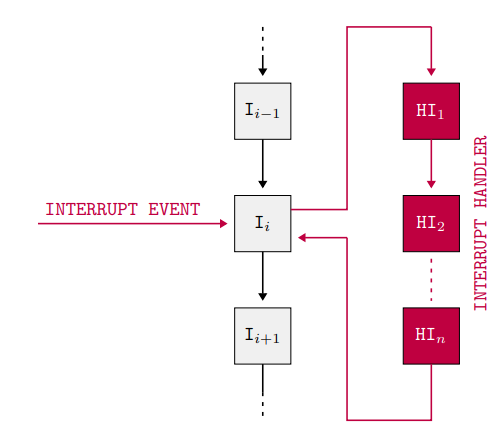
\includegraphics{Images/Screenshot 2023-05-16 123043.png}
  \caption{Interrupt event}
  \label{fig:interrupt-event}
  \bigskip
\end{figure}

% unbreakable list
\begin{minipage}{0.99\textwidth}
  \bigskip
  The interrupts can be:
  \begin{itemize}
    \item \textbf{Asynchronous}: created by an \textbf{external event}, for example:
          \begin{itemize}
            \item input or output device service request
            \item timer expiration
            \item power disruption or hardware failure
          \end{itemize}
    \item \textbf{Synchronous}: created by an \textbf{internal event}, for example:
          \begin{itemize}
            \item undefined \textit{opcode}, arithmetic overflow, \textit{FPU} exception
            \item privileged instruction, misaligned memory access
            \item virtual memory exceptions
                  \begin{itemize}
                    \item page faults
                    \item \textit{TLB} misses
                    \item protection violations
                  \end{itemize}
            \item traps
                  \begin{itemize}
                    \item system calls
                    \item jumps to kernel
                  \end{itemize}
          \end{itemize}
  \end{itemize}
  \bigskip
\end{minipage}

Synchronous events are also called \textbf{Exceptions}.

\subsection{Precise Interrupts}

An interrupt or exception is considered precise if there is a single instruction \textit{(or interrupt point)} for which all instructions before that one have committed their state and no following instructions \textit{(including the interrupting one)} have modified any state.

This effectively implies that the execution can be restarted at the interrupt point and continue correctly.

\bigskip
This kind of interrupt is desirable because:

\begin{itemize}
  \item Many types of interrupts or exceptions \textbf{need to be restartable}
  \item It's \textbf{easier to figure out what actually happened} and what caused the exception
\end{itemize}

While restartability does not require preciseness, it makes it a lot easier to restart the execution by:

\begin{itemize}
  \item Reducing the \textbf{number of states} to be saved if the process has to be unloaded
  \item Making \textbf{quicker restarts} due to the faster interrupts
\end{itemize}

\bigskip
The operation of an interrupt is shown in Figure~\ref{fig:operation-interrupt}.

\begin{figure}
  \bigskip
  \centering
  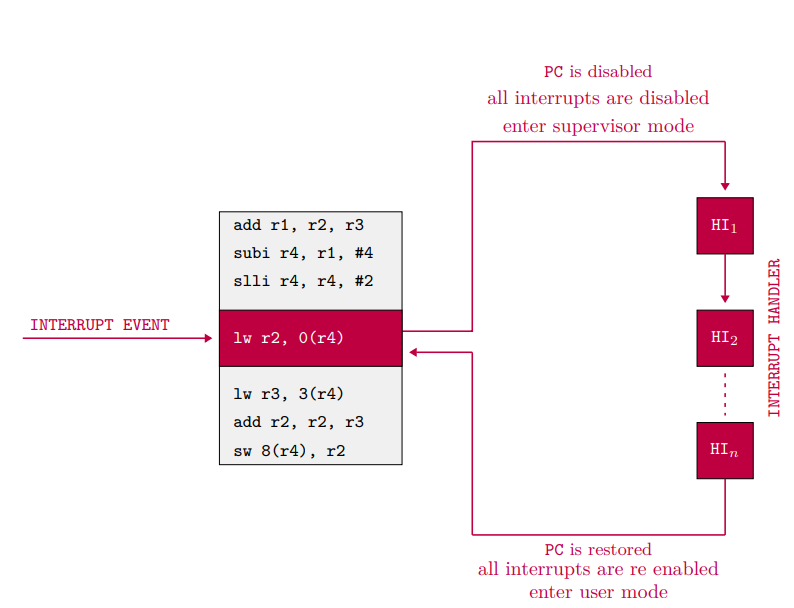
\includegraphics{Images/Screenshot 2023-05-16 123056.png}}
  \caption{Operation of an interrupt}
  \label{fig:operation-interrupt}
  \bigskip
\end{figure}

\subsection{Classes of Exceptions}

Exceptions can be divided into classes:

\begin{itemize}
  \item \textbf{Synchronous} and \textbf{Asynchronous}:
        \begin{itemize}
          \item Asynchronous exceptions are caused by devices external to the \textit{CPU} and memory and are easier to handle as they can be addressed after the current instruction
        \end{itemize}
  \item \textbf{User requested} and \textbf{Coerced}:
        \begin{itemize}
          \item User requested are predictable, they are treated as exceptions because they use the same mechanisms that are used to save and restore the state and are handled after the instruction has been completed
          \item Coerced exceptions are caused by some hardware event, not under the control of the program
        \end{itemize}
  \item \textbf{User Maskable} and \textbf{User Nonmaskable}:
        \begin{itemize}
          \item The mask controls whether the hardware responds to the exception or not
        \end{itemize}
  \item \textbf{Within} vs \textbf{Between} instructions:
        \begin{itemize}
          \item Exceptions that occur between instructions are usually synchronous as they are triggered by instruction. The instruction must be stopped and restarted
          \item Asynchronous that occur between instructions arise from catastrophic situations and cause program termination
        \end{itemize}
  \item \textbf{Resume} and \textbf{Terminate}
        \begin{itemize}
          \item With a terminating event, the program execution always stops
          \item With resuming events, the program execution continues after the interrupt
        \end{itemize}
\end{itemize}

\subsubsection{Asynchronous Interrupts}

The \textbf{Asynchronous Interrupts} work by:

\begin{enumerate}
  \item Invoking the \textbf{Interrupt Handler}
        \begin{itemize}
          \item an \textit{I/O} device requests attention by asserting one of the prioritized interrupt request lines
        \end{itemize}
  \item When the processor decides to \textbf{address the interrupt}, it has to:
        \begin{enumerate}[label=\arabic*.]
          \item stop the current program at instruction \(\texttt{I}_i\)
          \item complete all the instructions up until \(\texttt{I}_{i-1}\) \textit{(precise interrupt)}
          \item save the \texttt{PC} of instruction \(\texttt{I}_i\) in a special register called \textit{EPC}
          \item disable interrupts and transfer control to a designated interrupt handler running in the kernel mode
        \end{enumerate}
\end{enumerate}

Then the operation is handled by the \textbf{Interrupt Handler}, which will:

\begin{enumerate}[resume*]
  \item \textbf{Save} the \textit{PC} before enabling interrupts to allow nested interrupts
        \begin{itemize}
          \item it needs an instruction to move the \texttt{PC} into \textit{GPRs}
          \item it needs a way to mask further interrupts at least until the \texttt{PC} can be saved
        \end{itemize}
  \item \textbf{Read} a \textit{status register} that indicates the cause of the interrupt
  \item \textbf{Use} a special indirect jump instruction (\texttt{RFE}, \textit{Return From Exception}) which:
        \begin{itemize}
          \item enables interrupts
          \item restores the processor to the user mode
          \item restores hardware status and control state
        \end{itemize}
\end{enumerate}

\subsubsection{Synchronous Interrupts}

A \textbf{Synchronous Interrupt} is caused by a \textbf{particular} instruction.
Generally, the instruction \textbf{cannot be completed} and needs to be \textbf{restarted} after the exception has been handled.
This procedure requires undoing the effect of one or more partially executed instructions.

In case the interrupt was raised by a system call trap \textit{(a special jump instruction involving a change to privileged kernel mode)}, the instruction is considered to have been completed.

\subsection[Precise interrupts in 5 stages pipeline]{Precise interrupts in \(5\) stages pipeline}

Exceptions may occur at different stages in the pipeline, due to the out-of-order executions.
For instance, \textit{arithmetic exceptions} occur in \texttt{EX} stage, while \textit{TLB faults} occur in \texttt{IF} or \texttt{ME} stages.

The same issue arises while handling interrupts, as the pipeline must be interrupted as little as possible.

This problem can be solved by tagging instructions in the pipeline as \inlinequote{cause exceptions or not} and waiting until the end of \texttt{ME} stage to flag exceptions.
Then:

\begin{itemize}
  \item Interrupts become marked \texttt{NOP} \textit{(like bubbles)} that are placed into pipeline instead of an instruction
  \item Interrupt conditions are assumed to be persistent in case of flushed \texttt{NOP} instructions
  \item A clever \texttt{IF} stage might start fetching instructions from the interrupt vector
        \begin{itemize}
          \item this step is complicated by the need for supervisor mode switch, saving multiple \texttt{PC} and more similar issues
        \end{itemize}
\end{itemize}

\bigskip
In detail, exceptions are handled by:

\begin{itemize}
  \item Holding exceptions flags in pipeline until the commit point \textit{(\texttt{ME} stage)}
  \item Overriding newer exceptions for given instructions with older exceptions
  \item Injecting external interrupts at commit point, overriding other interrupts
  \item If an exception happens at commit, updating \textit{CAUSE} and \textit{ECP} registers, killing all stages and injecting handler \texttt{PC} into \texttt{IF} stage
\end{itemize}

While dealing with an in-order pipeline might be easy, generating a precise interrupt when instructions are being executed in an arbitrary order is not as easy.
In his famous paper, \textit{Jim Smith} proposes \(3\) methods for getting precise interrupts:

\begin{itemize}
  \item In-order instruction completion
  \item Reorder buffer
  \item History buffer
\end{itemize}

\subsubsection{Speculating on Exceptions}

There are \(3\) technique to speculate on exceptions:

\begin{itemize}
  \item \textbf{Prediction} mechanism
        \begin{itemize}[label=\(\rightarrow\)]
          \item exceptions are so rare that predicting no exceptions is surprisingly accurate
        \end{itemize}
  \item C\textbf{heck Prediction} mechanism
        \begin{itemize}[label=\(\rightarrow\)]
          \item exceptions are detected at the end of the instruction execution pipeline
          \item dedicated hardware for different exception types
        \end{itemize}
  \item \textbf{Recovery} mechanism
        \begin{itemize}[label=\(\rightarrow\)]
          \item only write architectural state at commit point, so partially executed instruction can be thrown away after exception
          \item exception handler is launched only after the pipeline is flushed
        \end{itemize}
\end{itemize}

\clearpage
\section{Instruction Level Parallelism - \textit{ILP}}

The objective of the \textit{ILP} is to improve the \textit{CPI}, with the ideal goal of \(1\) \textit{cycle per instruction}.

The \textit{ILP} implies a potential overlap of execution among unrelated instructions. This is achievable if there are no hazards.

\subsection{Multi-Cycle Pipeline}
Pipeline going in order, we keep one instruction at the time in sequential order. On instruction from sequential flow, one by one.

We can have two cases:
\begin{itemize}
    \item Execution stage: could be multiple cycle.
For example: Multiply or divide operation in the alu require more the 1 clk cycle.
\item Memory stage: require multiple cycle , this are caused by cache misses, this could cause that it will take 10 or 20 clock cycles.
\end{itemize}
\subsubsection{In-order commit}
This means that i do not care in which order they are executed, if one is faster then the other, but i need to commit with the flow order.

Otherwise, if I use out-of-order i need to implement some logic to accept those  type of commit, to preserve the absense\footnote{assenza? forse} of conflict like \textit{WAR & WAW}
\subsubsection{Difference between MIPS and Multi-ISSUE}
In \textit{MIPS} decode and access to the register were in the same \textit{CLK}, now we add another stage that is goal is to issue the instruction and pipeline in the correct \textit{Functional Unit}.

In this way I can commit in out-of-order with all of the problems that occurs.
\begin{figure}[h!]
    \centering
    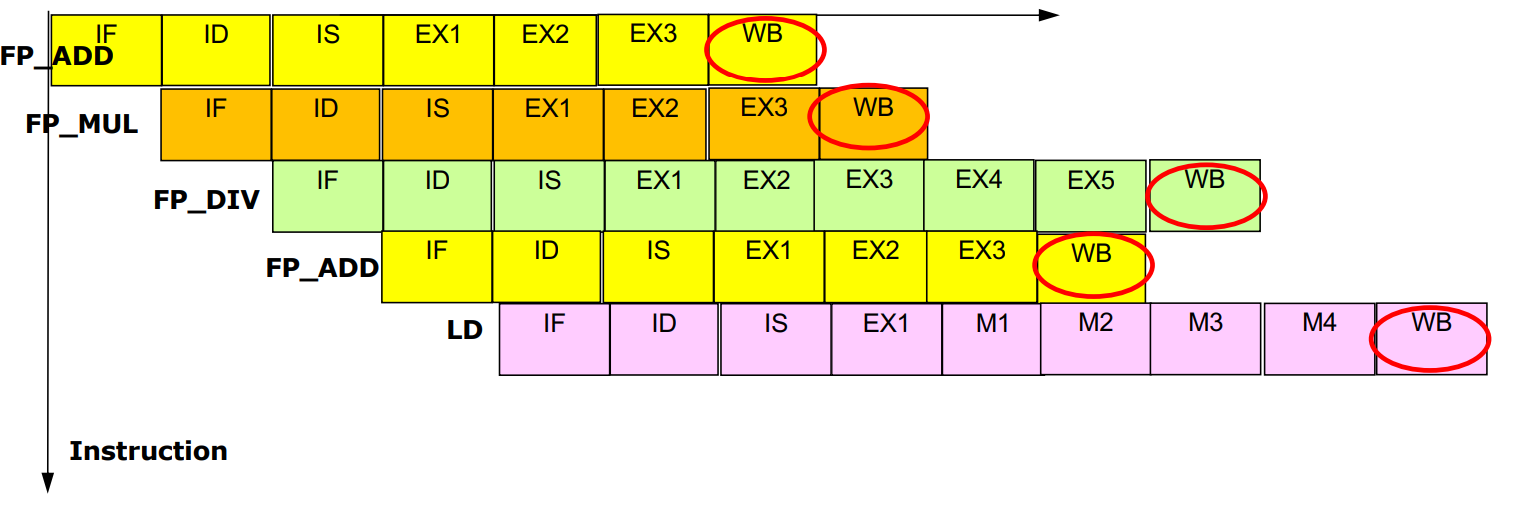
\includegraphics[scale = 0.5]{Images/Screenshot 2023-05-30 110220.png}
    \caption{In-order issue / out-of-order commit}
    \label{fig:my_label}
\end{figure}

\clearpage
\subsection{Dual-Issue Pipeline}
At each clock we will fetch and decode two instruction, but can be more, so we have to modify our register file to handle this request.
\begin{figure}[h!]
    \centering
    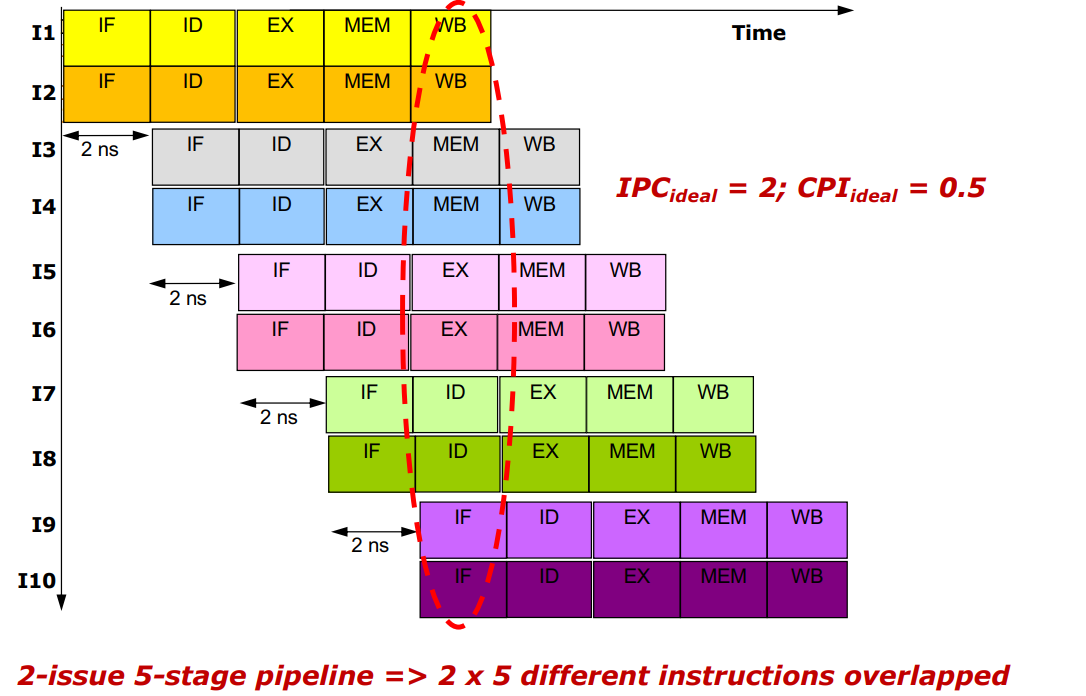
\includegraphics[scale=0.5]{Images/Screenshot 2023-05-30 141343.png}
    \caption{Dual Issue pipeline}
    \label{fig:my_label}
\end{figure}
Since we ave a single thread / single process we have to use a register file with 4 read/write port to write 2 results.

Also the fetch of instruction cache is double the size. Also forwarding path are more complicated.
\subsection{Strategies to support \textit{ILP}}
\label{sec:strategies-to-support-ilp}

There are main two software strategies to support \textit{ILP}:

\begin{enumerate}
  \item \textbf{Dynamic} scheduling: depends on the hardware to locate parallelism
  \item \textbf{Static} scheduling: relies on the software to identify potential parallelism
\end{enumerate}

Usually, hardware-intensive approaches dominate desktop and server markets.

\subsubsection{Dynamic scheduling}

The hardware reorders the instruction execution to reduce pipeline stall while maintaining data flow and exception behaviour.

\bigskip
\textit{Properties of the Dynamic Scheduling}:

\begin{enumerate}
  \item Instructions are fetched and \textbf{issued in program order}
  \item Execution begins \textbf{as soon as operands are available}, possibly out of order execution
  \item Out of order execution introduces possibility or \textit{WAR} and \textit{WAW} data hazards
  \item Out of order execution implies \textbf{out of order completion}
        \begin{itemize}
          \item a \textit{reorder buffer} is needed to reorder the output
        \end{itemize}
\end{enumerate}


\bigskip
\textbf{Advantages} of dynamic scheduling:
\begin{itemize}
  \item It enables handling some cases where dependencies are \textbf{unknown} at compile time
  \item It \textbf{simplifies} the compiler complexity
  \item It allows compiled code to run \textbf{efficiently} on a different pipeline
\end{itemize}

\textbf{Disadvantages}:
\begin{itemize}
  \item A significant increase in \textbf{hardware complexity}
  \item Increased \textbf{power consumption}
  \item Could generate \textbf{imprecise exception}
\end{itemize}

\subsubsection{Scoreboard}
\label{par:CDC6600-scoreboard}

A specific data structure is needed to solve data dependences without specialized compilers.
The first implementation of such hardware is found in the \textbf{Scoreboard}, created in \textit{1963}.

Its key idea is to allow instruction behind stalls to proceed, with the result of a \(250\%\) speedup with regards to no dynamic scheduling and a \(170\%\) speedup with regards to instructions reordering by the compiler.
It has the downside of having a \textbf{slow memory} \textit{(due to the absence of cache)} and \textbf{no forwarding hardware}.
Furthermore, it has a low number of \textit{FUs} and it does not issue structural hazards.

It solves the issue of data dependencies that cannot be hidden with bypassing or forwarding due to the hardware stalls of the pipeline by allowing out-of-order execution and commit of instructions.

\bigskip
The scoreboard centralizes hazard management.
It can avoid them by:

\begin{itemize}
  \item Dispatching \textbf{instructions} in order to functional units provided there's no structural hazard or \textit{WAW}
        \begin{itemize}
          \item a \textbf{stall} is added on structural hazards \textit{(when no functional unit is available)}
          \item there can be only one pending write to each register
        \end{itemize}
  \item Instructions \textbf{wait} for input operands to avoid \textit{RAW} hazards
        \begin{itemize}
          \item as a result, it can execute out-of-order instructions
        \end{itemize}
  \item Instructions \textbf{wait} for output register to be read by preceding instructions to avoid \textit{WAR} hazards
        \begin{itemize}
          \item results are held in functional units until the register is freed
        \end{itemize}
\end{itemize}

\bigskip
The scoreboard is operated by:

\begin{enumerate}
  \item \textbf{Sending} each instruction through it
  \item \textbf{Determining} when the instruction can read its operands and subsequently start its execution
  \item \textbf{Monitoring} changes in hardware and deciding when a stalled instruction can execute
  \item \textbf{Controlling} when instruction can write results
\end{enumerate}

As a result, a new pipeline is introduced, where the \texttt{ID} stage is divided into two parts:
\begin{enumerate}
  \item \textit{issue}, where the instruction is decoded and \textbf{structural hazards} are checked
  \item \textit{read operands}, where the operation waits until there are no \textbf{data hazards}
\end{enumerate}

Finally, the scoreboard is structured in three different parts:
\begin{enumerate}
  \item \textbf{Instruction} status
  \item \textbf{Functional Units} status
        \begin{itemize}
          \item fields indicating the state of each \textit{FUs}:
                \begin{itemize}
                  \item \texttt{Busy} - indicates whether the unit is busy or not
                  \item \texttt{Op} - the operation to perform in the unit
                  \item \texttt{Fi} - the destination register
                  \item \texttt{Fj}, \texttt{Fk} - source register numbers
                  \item \texttt{Qj}, \texttt{Qk} - functional units producing source registers
                  \item \texttt{Rj}, \texttt{Rk} - flags indicating when \texttt{Fj}, \texttt{Fk} are ready
                \end{itemize}
        \end{itemize}
  \item \textbf{Register} result status
        \begin{itemize}
          \item indicates which functional unit will write each register
          \item it's \texttt{blank} if no pending instructions will write that register
        \end{itemize}
\end{enumerate}

\bigskip
An illustration of the new pipeline is represented in Figure~\ref{fig:pipeline-of-scoreboard}, while the structure of the scoreboard is represented in Figure~\ref{fig:structure-of-scoreboard}.

\begin{figure}[htbp]
  \bigskip
  \centering
  \tikzfig[1]{image-24.tikz}
  \caption{Pipeline introduced by the \textit{Scoreboard}}
  \label{fig:pipeline-of-scoreboard}
  \bigskip
\end{figure}

\begin{figure}[htbp]
  \bigskip
  \centering
  \tikzfig[1]{image-25.tikz}
  \caption{Structure of the \textit{Scoreboard}}
  \label{fig:structure-of-scoreboard}
  \bigskip
\end{figure}

\paragraph{Four stages of Scoreboard Control}

The four stages of scoreboard control are:

\begin{itemize}
  \item \textbf{Issue}: instructions are decoded and structural hazards \textit{(WAW)} are checked for
        \begin{itemize}
          \item instructions are issued in program order for hazard checking
          \item if the \textit{FU} for the instruction is free and no other active instruction has the same destination register, the scoreboard issues the instruction and updates its internal data structure
          \item if a structural or \textit{WAW} hazard exists, then the instruction issue stalls and no further instructions are issued until they are solved
        \end{itemize}
  \item \textbf{Read operands}: expiration of data hazards is awaited, then operands are read
        \begin{itemize}
          \item a source operand if available if no earlier issued active instruction will write it or a functional unit is writing its value into a register
          \item when the source operands are available, the scoreboard tells the \textit{FU} to proceed to read the operands from the registers and begin execution
          \item \textit{RAW} hazards are resolved dynamically, instructions could be sent out of order
          \item there's no data forwarding in this model
        \end{itemize}
  \item \textbf{Execution}: the \textit{FUs} operate on the data
        \begin{itemize}
          \item when the result is ready, the scoreboard it's notified
          \item the delays are characterized by \textbf{latency} and \textbf{initiation interval}
        \end{itemize}
  \item \textbf{Write result}: the execution is finished
        \begin{itemize}
          \item once the scoreboard is aware that the \textit{FU} has completed the execution, it checks for \textit{WAR} hazards
                \begin{itemize}
                  \item if no \textit{WAR} hazard is found, the result is written
                  \item otherwise, the execution is stalled
                \end{itemize}
          \item \textbf{issue} and \textbf{write} stages can overlap
        \end{itemize}
\end{itemize}

\bigskip
This structure creates a few implications:

\begin{itemize}
  \item \textit{WAW} are \textbf{detected} \textit{(and the pipeline is stalled)} until the other instruction is completed
  \item There's \textbf{no register renaming}
  \item \textbf{Multiple instructions must be dispatched} in the execution phase, creating the need for multiple or pipelined execution units
  \item Scoreboard \textbf{keeps track of dependences} and the state of the operations
\end{itemize}

\subsubsection{Tomasulo algorithm}

The Tomasulo algorithm is a \textbf{dynamic} algorithm that allows execution to proceed in presence of dependences.

The key idea behind this algorithm is to \textbf{distribute} the control logic and the buffers within \textit{FUs}, as opposed to the scoreboard \textit{(in which the control logic is centralized)}.

The operand buffers are called \textbf{Reservation Stations} \textit{(RS)}:
each instruction is also an entry to a \textit{RS} and its operands are replaced by values or pointers \textit{(a technique known as \textbf{Implicit Register Renaming})} in order to avoid \textit{WAR} and \textit{RAW} hazards.

Results are then dispatched to other \textit{FUs} through a \textit{Common Data Bus}, communicating both the data and the source.
Finally, \texttt{LOAD} and \texttt{STORE} operations are treated as \textit{FUs}, as \textit{RS} are more complex than architectural registers to allow more compiler-level optimizations.

\paragraph{Structure of the Reservation Stations}

The Reservation Station is composed by \(5\) \textbf{fields}:

\begin{itemize}
  \item \texttt{TAG} - indicating the \textit{RS} itself
  \item \texttt{OP} - the operation to perform in the unit
  \item \texttt{Vj}, \texttt{Vk} - the value of the source operands
  \item \texttt{Qj}, \texttt{Qk} - pointers to the \textit{RS} that produces \texttt{Vj}, \texttt{Vk}
        \begin{itemize}
          \item its value is zero if the source operator is already available in \texttt{Vj} or \texttt{Vk}
        \end{itemize}
  \item \texttt{BUSY} - indicates the \textit{RS} is busy
\end{itemize}

In this description, only one between the \texttt{V}-field and the \texttt{Q}-field is valid for each operand.

\bigskip
Furthermore, a few more components are needed, such as:

\begin{itemize}
  \item \textbf{Register File} and the \textbf{Store} buffers have a \textit{Value} (\texttt{V}) and a \textit{Pointer} (\texttt{Q}) field
        \begin{itemize}
          \item \texttt{Q} corresponds to the number of the \textit{RS} producing the result (\texttt{V}) to be stored in \textit{Register File} or \textit{Store} buffers
          \item if \texttt{Q = 0}, no active instructions is producing a result and the \textit{Register File} \textit{(or \texttt{STORE})} buffer contains the wrong value
        \end{itemize}
  \item \textbf{Load} and \textbf{Store} buffers have an \textit{Address} (\texttt{A}) field, with the former having also a \textit{Busy} field \textit{(\texttt{BUSY})}
        \begin{itemize}
          \item the \texttt{A} field holds information for memory address calculation: initially contains the instruction offset, while after the calculation it stores the effective address
        \end{itemize}
\end{itemize}

\paragraph{Stages of the Tomasulo Algorithm}

The Tomasulo algorithm is structured in \(3\) different stages: \textbf{Issue}, \textbf{Execute} and \textbf{Write}.

\bigskip
In more detail:

\begin{enumerate}
  \item \textbf{Issue} stage:
        \begin{itemize}
          \item Get an instruction \texttt{I} from the queue
                \begin{itemize}
                  \item if it is an \textit{FP} operation, check if any \textit{RS} in empty \textit{(i.e. check for any structural hazard)}
                \end{itemize}
          \item Rename the registers
          \item Resolve \textit{WAR} hazards
                \begin{itemize}
                  \item if \texttt{I} writes \textit{R}, read by an already issued instruction \texttt{K}, \texttt{K} will already know the value of \textit{R} or knows that instruction will write into it
                  \item the \textit{Register File} can be linked to \texttt{I}
                \end{itemize}
          \item Resolve \textit{WAW} hazards
                \begin{itemize}
                  \item since the in-order issue is used, the \textit{Register File} can be linked to \texttt{I}
                \end{itemize}
        \end{itemize}
  \item \textbf{Execute} stage:
        \begin{itemize}
          \item When both the operands are ready, then the operation is executed. Otherwise, watch the \textit{Common Data Bus} for results.
                \begin{itemize}
                  \item by delaying the execution until both operands are available, \textit{RAW} hazards are avoided
                  \item several instructions could become ready in the same clock cycle for the same \textit{FU}
                \end{itemize}
          \item \texttt{LOAD} and \texttt{STORE} are two-step processes:
                \begin{itemize}
                  \item effective address is computed and placed in \texttt{LOAD/STORE} buffer
                  \item \texttt{LOAD} operations are executed as soon as the memory unit is available
                  \item \texttt{STORE} operations wait for the value to be stored before sending it into the memory unit
                \end{itemize}
        \end{itemize}
  \item \textbf{Write} stage:
        \begin{itemize}
          \item When the result is available, it is written on the \textit{Common Data Bus}
                \begin{itemize}
                  \item it is then propagated into the \textit{Register File} and all the registers \textit{(including \texttt{STORE} buffers)} waiting for this result
                  \item \texttt{STORE} operations write data to memory
                  \item \textit{RSs} are marked as available
                \end{itemize}
        \end{itemize}
\end{enumerate}

\paragraph{Focus on \texttt{LOAD} and \texttt{STORE} in Tomasulo Algorithm}

\texttt{LOAD} and \texttt{STORE} instructions go through a functional unit for effective computation before proceeding to their respective load and \texttt{STORE} buffers.
\texttt{LOAD} take a second execution step to access memory, then go to \textit{Write} stage to send the value from memory to \textit{Register File} and/or \textit{RS}, while \texttt{STORE} complete their execution in their \textit{Write} stage.
All write operations occur in the write stage, thus simplifying the algorithm.

\bigskip
A \texttt{LOAD} and a \texttt{STORE} instruction can be done in a different order, provided they access different memory locations.
Otherwise, a \textit{WAR} \textit{(interchange in load-store sequence)} or a \textit{RAW} \textit{(interchange in store-load sequence)} may result in a  \textit{WAW} \textit{(if two stores are interchanged)}.
However, \texttt{LOAD} instructions can be reordered freely.

To detect such hazards, data memory addresses associated with any earlier memory operation must have been computed by the \textit{CPU}.

\bigskip
\texttt{LOAD} instructions executed out of order with previous \texttt{STORE} assume that the address is computed in program order.
When the \texttt{LOAD} address has been computed, it can be compared with \texttt{A} fields in active \texttt{STORE} Buffers: in case of a match, the load is not sent to its buffer until conflicting \texttt{STORE} completes.

Store instructions must check for matching addresses in both \texttt{LOAD} and \texttt{STORE} buffers.
This is a \textbf{dynamic disambiguation} and, opposing to the static disambiguation, is not performed by the compiler.
As a drawback, more hardware is required to perform these operations: each \textit{RS} must contain a fast associative buffer, because single \textit{CDB} \textit{(Common Data Bus)}  may limit performance.

\paragraph{Tomasulo and Loops}

Tomasulo algorithm can \textbf{overlap} iterations of loops due to:

\begin{itemize}
  \item \textbf{Register Renaming}
        \begin{itemize}
          \item \textbf{multiple iterations} use \textbf{different physical destinations} for registers
          \item \textbf{static register names are replaced} from code with dynamic registers \textit{"pointers"}, effectively increasing the size of the register file
          \item \textbf{instruction issue is advanced} past integer control flow operations
        \end{itemize}
  \item \textbf{Fast branch resolution}
        \begin{itemize}
          \item integer unit must \textit{"get ahead"} of floating point unit so that multiple iterations can be issued
        \end{itemize}
\end{itemize}

\paragraph{Comparison between Tomasulo Algorithm and Scoreboard}

The main advantages of the Tomasulo algorithm over the scoreboard are:

\begin{itemize}
  \item Control and buffers are \textbf{distributed} with \textit{FUs}
        \begin{itemize}
          \item \textit{FUs} buffers are called \textbf{reservation stations} and have pending operands
        \end{itemize}
  \item Registers in instructions are \textbf{replaced} by values or pointers to \textit{RS}
        \begin{itemize}
          \item avoids \textit{WAR} and \textit{WAW} hazards
          \item since there are more \textit{RS} than registers, there's a higher optimization than compilers alone can do
        \end{itemize}
  \item The result are \textbf{propagated} from \textit{RS} to \textit{FU} via \textit{Common Data Bus}
        \begin{itemize}
          \item the value is propagated \textbf{to all \textit{FUs}}
        \end{itemize}
  \item \texttt{LOAD} and \texttt{STORE} instructions are treated as \textit{FUs} with \textit{RSs}
  \item Integer instructions can go past \textbf{branches}, allowing \textit{FP} ops beyond basic block in \textit{FP} queue
\end{itemize}

\subsection{Limits of \textit{ILP}}

In order to execute more than one instruction at the beginning of a clock cycle, two requirements must be satisfied:

\begin{enumerate}
  \item Fetching more than one \textbf{instruction per clock cycle}
        \begin{itemize}
          \item this task is completed by the \textit{Fetch Unit}
          \item there is no major problem provided the instruction cache \textit{(I-cache)} can sustain the bandwidth and can manage multiple requests at one
        \end{itemize}
  \item Decide on data and control \textbf{dependences}
        \begin{itemize}
          \item \textit{dynamic scheduling} and \textit{dynamic branch prediction} are needed
        \end{itemize}
\end{enumerate}

Superscalar architectures paired with compiler scheduling can achieve such speeds.

\bigskip
A few requirements must be satisfied to start an ideal machine:

\begin{enumerate}
  \item \textbf{Register renaming}
        \begin{itemize}
          \item by using an infinite number of virtual registers, all \textit{WAW} and \textit{WAR} hazards are avoided
        \end{itemize}
  \item \textbf{Branch prediction}
        \begin{itemize}
          \item by using a perfect predictor, no branch is ever mispredicted
        \end{itemize}
  \item \textbf{Jump prediction}
        \begin{itemize}
          \item all jumps are perfectly predicted
          \item a machine with perfect speculation and an infinite buffer of instructions is needed
        \end{itemize}
  \item \textbf{Memory address alias analysis}
        \begin{itemize}
          \item addresses are known and a \texttt{STORE} can be moved before a \texttt{LOAD} if their addresses are different
        \end{itemize}
  \item \textbf{\(1\) cycle latency} for all instructions
        \begin{itemize}
          \item an unlimited number of instructions can be issued each clock cycle
        \end{itemize}
\end{enumerate}

\subsubsection{Initial assumptions}

Furthermore, a few \textbf{initial assumptions} must be made:

\begin{itemize}
  \item \textit{CPU} can issue an\textbf{ unlimited number of instructions}, looking arbitrarily far ahead in the computation
  \item There's \textbf{no restriction on types of instructions} that can be executed in one cycle \textit{(including loads and stores)}
  \item All \textit{FUs} \textbf{have unitary latency}: any sequence of depending instructions can issue on successive cycles
  \item All \textit{LOAD} and \textit{STORE} execute in \(1\) cycle, thanks to perfect caches
\end{itemize}

\subsubsection{Limits dynamic analysis}

\textbf{Dynamic analysis} is necessary to approach perfect branch prediction, and it cannot be achieved at compile time.
A perfect dynamic scheduled \textit{CPU} should:

\begin{enumerate}
  \item \textbf{Look arbitrarily far ahead} to find a set of instructions to issue and predict all branches perfectly
  \item \textbf{Rename all registers} in use, avoiding all \textit{WAR} and \textit{RAW} hazards
  \item Determine whether there are \textbf{data dependences among instructions} in the issue packet, renaming them if necessary
  \item Determine and handle all \textbf{memory dependences among issuing instructions}
  \item \textbf{Provide} enough replicated \textbf{functional units} to allow all ready instructions to issue
\end{enumerate}

\subsection{Static Scheduling}

Compilers can use sophisticated algorithms for code scheduling to exploit \textit{ILP}.
The amount of parallelism available within a basic block \textit{(a straight line code sequence with no branches in except to the entry and no branches out except at the exit)} is quite small, and
data dependence can further limit the amount of \textit{ILP} that can be exploited within a basic block much less than the average basic block size.
To obtain substantial performance enhancements, \textit{ILP} must be exploited across multiple basic blocks \textit{(i.e. across branches)}.

The static detection and resolution of dependencies are accomplished by the compiler, so they are avoided by code reordering.
The compiler outputs dependency-free code.

\bigskip
\textbf{Limits of static scheduling}:
\begin{itemize}
  \item \textbf{Unpredictable} branches
  \item Variable memory \textbf{latency} \textit{(due to unpredictable cache misses)}
  \item Huge increase in \textbf{code size}
  \item High compiler \textbf{complexity}, because all of the scheduling logic is  related to compiler\footnote{FLC potrebbe servire a qualcosa}.

\end{itemize}
\subsection{SuperScalar architectures}
This type of  architectures need a complex hardware, because they are static scheduled. This means a large area and energy consumption, this need a large instruction window. 

The data dependency are managed at execution time.
\subsection{VLIW architectures}

The \textbf{Very Long Instruction Words} \textit{(VLIW)} is a particular architecture made specifically to fetch more instructions at a time.
The \textit{CPU} issues multiple sets of operations \textit{(single unit of computations, such as \texttt{ADD}, \texttt{LOAD}, \texttt{branch}, \ldots) }called \textbf{instructions}.
Those are meant to be intended to be issued at the same time and the compiler has to specify them completely.

\bigskip
Its features include:

\begin{itemize}
  \item \textbf{Fixed number} of instructions \textit{(between \(4\) and \(16\))}
  \item The instructions are scheduled by the \textbf{compiler}
        \begin{itemize}
          \item the hardware has \textbf{very limited control} on what is going on
          \item the instructions are going to have a \textbf{very low dependency}
        \end{itemize}
  \item The operations are put into wide \textbf{templates}
  \item \textbf{Explicit} parallelism
        \begin{itemize}
          \item parallelism is found at compile time, not run time
          \item the compiler is responsible for parallelizing the code, not the designer
        \end{itemize}
  \item Single \textbf{control flow}
        \begin{itemize}
          \item there's only one \texttt{PC}
          \item only one instruction is issued each clock cycle
        \end{itemize}
  \item Low hardware \textbf{complexity}
        \begin{itemize}
          \item there's no need to to perform \textit{scheduling} or \textit{reordering} on hardware level
          \item all operations that are supposed to begin at the same time are packaged into a single instruction
          \item each operations slot is meant for a fixed functions
          \item constant operation latencies are specified
        \end{itemize}
\end{itemize}

There are multiple \textbf{functional units} \textit{(FUs)} that are going to execute instructions in parallel.
An illustration of the inner working instruction level is represented in Figure~\ref{fig:vliw-instruction-level}, while the pipeline level is represented in Figure~\ref{fig:vliw-pipeline-level}.

\begin{figure}[htbp]
  \bigskip
  \centering
  \tikzfig[1]{image-26.tikz}
  \caption{\textit{VLIW} - instructions level}
  \label{fig:vliw-instruction-level}
  \bigskip
\end{figure}

\begin{figure}[htbp]
  \bigskip
  \centering
  \tikzfig[1]{image-27.tikz}
  \caption{\textit{VLIW} - pipeline level}
  \label{fig:vliw-pipeline-level}
  \bigskip
\end{figure}

\subsubsection{Compiler responsibilities}

The \textbf{compiler} has to schedule the instructions \textit{(via \textbf{static scheduling})} to maximize the parallel execution:

\begin{itemize}
  \item It can exploit \textit{ILP} and \textit{LLP} \textit{(Loop Level Parallelism)}
  \item It is necessary to \textbf{map the instructions} over the machine functional units
  \item This mapping must account for \textbf{time constraints and dependences} among the tasks themselves
\end{itemize}

The idea behind the static scheduling in \textit{VLIW} is to utilize all functional units \textit{(FUs)} in each cycle as much as possible to reach a better \textit{ILP} and therefore higher parallel speedups.

\subsubsection{Basic Blocks and Trace Scheduling}
\label{sec:trace-scheduling}

Compilers use sophisticated algorithms to schedule code and exploit \textit{ILP}.
However, the amount of parallelism available in a single \textbf{basic block}, as previously pointed out, is quite small; furthermore, \textbf{data dependence} can limit the amount of \textit{ILP} that can be exploited to less than the average block size.

A \textbf{basic block} \textit{(BB)} is defined as a sequence of straight non-branch instructions.

In order to obtain substantial performance enhancements, the \textit{ILP} must be exploited across multiple blocks (\textit{i.e.} among branches).
An illustration of the structure of \textit{BB} can be found in Figure~\ref{fig:basic-blocks}.

\bigskip
A \textbf{trace} is a sequence of basic blocks embedded in the control flow graph.
It must not contain loops but it can include branches.

It's an \textbf{execution path} which can be taken for a certain set of inputs.
The chances that a trace is executed depend on the input set that allows its execution.
As a result, some traces are executed much more frequently than others.

The tracing scheduling algorithm works as follows:

\begin{enumerate}
  \item Pick a \textbf{sequence of basic blocks} that represents the most frequent branch path
  \item Use \textbf{profiling feedback} or compiler heuristics to find the common branch paths
  \item \textbf{Schedule} the whole trace at once
  \item Add \textbf{code to handle branches} jumping out of trace
\end{enumerate}

Scheduling in a trace relies on basic code motion but it could also use globally scoped code by appropriately \textit{renaming} some blocks.
Compensation codes are then needed for \textbf{side entry points} \textit{(i.e. points except beginning)} and \textbf{slide exit points} \textit{(i.e. points except the ending)}.

Blocks on non-common paths may now have added overhead, so there must be a high probability of taking common paths according to the profile.
However, this choice might not be clear for some programs.

In general, compensation codes are not easy to generate for entry points.

\bigskip
A comparison of scheduled and unscheduled codes can be found in Figure~\ref{fig:compare-scheduled-unscheduled-code}.

\begin{figure}[htbp]
  \bigskip
  \centering

  \begin{subfigure}[b]{0.495\textwidth}
    \centering
    \tikzfig[0.7]{image-28.tikz}
    \caption{Basic blocks}
    \label{fig:basic-blocks}
  \end{subfigure}
  \begin{subfigure}[b]{0.495\textwidth}
    \centering
    \tikzfig[0.7]{image-29.tikz}
    \caption{Trace scheduled code}
    \label{fig:trace-scheduled-code}
  \end{subfigure}
  \caption{Comparison of scheduled and unscheduled code}
  \label{fig:compare-scheduled-unscheduled-code}
  \bigskip
\end{figure}

\paragraph{Code motion and Rotating Register Files in Trace Scheduling}

In addition to the need for compensation codes, there are a few more restrictions on the movement of a code trace:

\begin{enumerate}[label=\Alph*), ref=(\Alph*)]
  \item \label{enum:data-flow-trace-scheduling} The \textbf{data flow} of the program must not change
  \item \label{enum:exception-behaviour-trace-scheduling} The \textbf{exception behaviour} must be preserved
\end{enumerate}

\bigskip

In order to ensure \ref{enum:data-flow-trace-scheduling}, the \textbf{Data} and \textbf{Control} dependency must be maintained.
Furthermore, control dependency can be eliminated using \textbf{predicate instructions} \textit{(via Hyperblock scheduling) }and branch removal or by using \textbf{speculative instructions} \textit{(via Speculative Scheduling)} and speculatively moving instructions before branches.

Finally, Trace Scheduling within loops requires lots of registers, due to the duplicated code:
to solve this issue, a new set of registers must be allocated for each iteration.

This solution is achieved via the use of \textbf{Rotating Register Files} \textit{(RRB)}.
The address of the \textit{RRB} register points to the base of the current register set.
The value added onto a local register specifier gives a physical register number.
\begin{figure}[htbp]
  \bigskip
  \centering
  \tikzfig[1]{image-30.tikz}
  \caption{Rotating Register File}
  \label{fig:rotating-register-file}
  \bigskip
\end{figure}

\subsubsection{Pros and cons of \textit{VLIW}}

\textit{Pros}:
\begin{itemize}[label=\cmarkthin]
  \item \textbf{Simple} \textit{HW}
  \item It's \textbf{easy} to increate the number of FU
  \item Good \textbf{compilers} can efficiently \textbf{detect parallelism}
\end{itemize}

\bigskip
\textit{Cons}:
\begin{itemize}[label=\xmarkthin]
  \item \textbf{Huge number of registers }to keep active each FU, each needed to store operands and results
  \item \textbf{Large data transport} capabilities between:
        \begin{itemize}
          \item FUs and register files
          \item register files and memory
        \end{itemize}
  \item H\textbf{igh bandwidth} between instruction cache and fetch unit
  \item \textbf{Large code} size
\end{itemize}

\subsubsection{Static Scheduling methods}

The static scheduling methods used in the \textit{VLIW} are:

\begin{itemize}
  \item Simple code \textbf{motion}
  \item \textbf{Loop unrolling} and loop peeling - \textit{Paragraph~\ref{par:loop-unrolling}}
  \item Software \textbf{pipelining} - \textit{Paragraph~\ref{par:software-pipelining}}
  \item Global code \textbf{scheduling} \textit{(across basic blocks)}
        \begin{itemize}
          \item \textbf{Trace} scheduling - \textit{Paragraph~\ref{par:trace-scheduling}}
          \item \textbf{Superblock} scheduling
          \item \textbf{Hyperblock} scheduling
          \item \textbf{Speculative} Trace scheduling
        \end{itemize}
\end{itemize}

\paragraph{Loop unrolling}
\label{par:loop-unrolling}
\subsubsection{Loop-Carried dependency}
To properly understand this section we need to catch this type of dependency.

They are really simple, to better understand see this code:
\begin{verbatim}
    for(int i = 1; i< N-1;i++){
        v[i] = v[i-1] + 50;
    }
\end{verbatim}
In this case we are using \texttt{v[i-1]} that is modified in the cycle before of the \textit{i-esimo} cycle\footnote{Semplicemente quando uso un dato fatto in un altro ciclo ho un grosso rischio} if a loop-carried dependecy occurs YOU DON'T HAVE TO APPLY AN LOOP-UNROLLING\footnote{Potrebbe servire anche in FLC, perchè se è presente una lista va sempre strotolata} 

Examine this snippet of code:

\begin{verbatim}
  for (int i = 0; i < N; i++)
    B[i] = A[i] + C;
\end{verbatim}

the inner loop gets \textit{unrolled} in order to execute \(4\) iterations at once:

\begin{verbatim}
  for (int i = 0; i < N; i += 4) {
    B[i] = A[i] + C;
    B[i + 1] = A[i + 1] + C;
    B[i + 2] = A[i + 2] + C;
    B[i + 3] = A[i + 3] + C;
  }
\end{verbatim}

A final clean-up is needed to take care of those values of \texttt{N} that are not multiples of the unrolling factor \textit{(\(4\) in this example)}.

This technique has the drawbacks of creating \textbf{longer code} and \textbf{losing performance} due to the costs of starting and closing each iteration.
Furthermore, trace scheduling cannot proceed beyond a loop.

With this technique, we have to be very careful with the index, because  this can be catastrophic.

\bigskip
An illustration of the performance improvements can be found in Figure~\ref{fig:performance-improvement-loop-unrolling}.

\begin{figure}[htbp]
  \bigskip
  \centering
  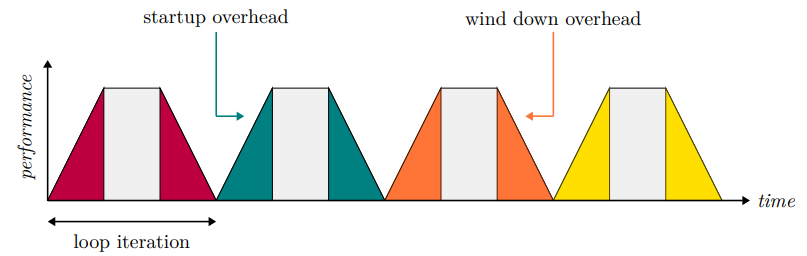
\includegraphics[]{Images/Screenshot 2023-05-16 123854.png}
  \caption{Performance improvement of loop unrolling}
  \label{fig:performance-improvement-loop-unrolling}
  \bigskip
\end{figure}

\paragraph{Software pipelining}
\label{par:software-pipelining}

The programs can be pipelined in order to increase performance and reduce the overall cost of the startup and wind down phases from once per iteration to once per loop.

\bigskip
An illustration of the performance improvements can be found in Figure~\ref{fig:performance-improvement-software-pipelining}.

\begin{figure}[htbp]
  \bigskip
  \centering
  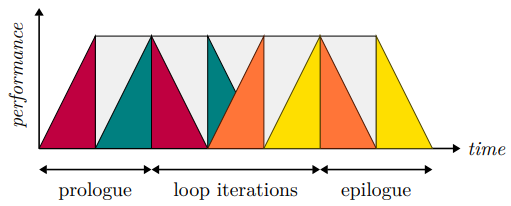
\includegraphics[]{Images/Screenshot 2023-05-16 123845.png}
  \caption{Performance improvement of software pipelining}
  \label{fig:performance-improvement-software-pipelining}
  \bigskip
\end{figure}

\paragraph{Trace scheduling}
\label{par:trace-scheduling}

As discussed in Section~\ref{sec:trace-scheduling}, Trace Scheduling 

To increase the performance in these situations, techniques based on loop unrolling are needed.
Traces scheduling schedules traces in order of decreasing probability of being executed.
As such, the most frequently executed traces get better schedules.

\clearpage
\section{Hardware Based Speculation}

The Hardware Based Speculation combines \(3\) ideas:

\begin{itemize}
  \item \textbf{Dynamic Branch Prediction} to choose which instruction to execute
  \item \textbf{Dynamic Scheduling} to support out-of-order execution while allowing in-order commit
        \begin{itemize}
          \item prevents irrevocable actions such as register update or exception taking until an instruction commits
        \end{itemize}
  \item \textbf{Speculation} to execute instructions before control dependencies are resolved
\end{itemize}

The outcome of the branches is speculated, and then the program is executed as if the speculation was correct.
Mechanisms are necessary to handle incorrect speculation: the hardware speculation extends dynamic scheduling beyond a branch \textit{(i.e. beyond the basic block)}.

\subsection{Reorder Buffer}

The \textbf{Reorder Buffer} \textit{(\textit{ROB})} holds instructions in \textit{FIFO} order, exactly as issued:
when the instructions are complete, their results are placed back in the \textit{ROB}.

Operands are supplied to the other instructions between their completion and their commit, while results are tagged with \textit{ROB} buffer number instead of the reservation station.

During the instruction commit, the values in the head of the \textit{ROB} are placed in registers.
This guarantee a speculative execution, so we can execute operation before their real time of execution \footnote{Ex. un ciclo while, eseguo la prima istruzione del ciclo ma potrei aver raggiunto la condizione per uscire e quindi quell'istruzione non serve, ecco questo è l'esecuzione speculative delle cose.}, but if the speculation goes wrong? Nothing happen, because the completion state is separed from commit state so we can undo everything.\\
With this hardware speculation we can obtain an in-order commit with out-of-order execution, manteining a precise interrupt/execption handling

\bigskip
\textit{ROB} is structured as a circular buffer with \textbf{head} and \textbf{tail} pointers.
Entries between those two are valid and they are allocated and freed whenever an instruction enters or leaves the \textit{ROB}.

Its main entries are:

\begin{itemize}
  \item The \textbf{type} of the instruction
  \item The \textbf{destination} register of the result
  \item The \textbf{result} of the instruction
  \item If any \textbf{exception} was raised
  \item The \textbf{program counter} \texttt{PC}
  \item If the \textbf{instruction} is \textbf{ready}
  \item If the \textbf{branch} is \textbf{speculative}
\end{itemize}
\begin{figure}[htpb]
  \bigskip
  \centering
  \begin{subfigure}[]{\textwidth}
    \centering
    \tikzfig[1]{image-33.tikz}
    \caption{\textit{ROB} structure}
    \label{subfig:structure-rob}
  \end{subfigure}
  \par\bigskip
  \begin{subfigure}[]{\textwidth}
    \centering
    \tikzfig[1]{image-34.tikz}
    \caption{\textit{ROB} entry}
    \label{subfig:rob-entries}
  \end{subfigure}
  \caption{Structure of the \textit{ROB} and its entries}
  \label{fig:structure-of-ROB}
  \bigskip
\end{figure}

\begin{minipage}{\textwidth}
  \bigskip
  The structure of an entry contains:

  \begin{itemize}
    \item The \texttt{TAG}, given by the index in the \textit{ROB}
    \item The new instructions are \textbf{dispatched} to free slot
    \item Instruction space is \textbf{reclaimed} when done by setting the \texttt{P} bit
    \item In \textbf{dispatch} stage:
          \begin{itemize}
            \item non-busy source operands are read from register files and copied to \texttt{SRC} fields where the \texttt{P} bit is set
            \item busy source operands copy \texttt{TAG} of producer and clear the \texttt{P} bit
            \item the \texttt{V} bit is set valid
          \end{itemize}
    \item In \textbf{issue} stage:
          \begin{itemize}
            \item the \texttt{I} bit is set valid
          \end{itemize}
    \item On \textbf{completion}:
          \begin{itemize}
            \item source tags are searched and the \texttt{P} bit is set
            \item result and \texttt{EXCEPTION} flags are written back to \textit{ROB}
          \end{itemize}
    \item On \textbf{commit}:
          \begin{itemize}
            \item \texttt{EXCEPTION} flags are checked
            \item \texttt{RESULT} is copied into register files
          \end{itemize}
    \item On \textbf{trap}:
          \begin{itemize}
            \item machine and \textit{ROB} are flushed
            \item \texttt{FREE} pointer is set as \texttt{OLDEST}
            \item the execution resumes from \texttt{HANDLER}
          \end{itemize}
  \end{itemize}
\end{minipage}

\bigskip
In order to separate the completion stage from the commit stage, the \textit{ROB} must hold register results from the former until the latter.

Each entry, allocated in program order during decode, holds:

\begin{itemize}
  \item The \textbf{type} of the instruction
  \item The \textbf{destination} register specifier and value \textit{(if any)}
  \item The \textbf{program counter}, \texttt{PC}
  \item The \textbf{exception} status \textit{(often compressed to save memory)}
\end{itemize}

They buffer completed values and exception states until the in-order commit point.
Completed values can be used by dependencies before reaching that point.

\subsubsection{Tomasulo's Algorithm and \textit{ROB}}

Tomasulo's Algorithm needs a buffer for all the uncommitted results.
It's structured as a \textit{ROB}.

Each entry of the \textit{ROB} contains \(4\) fields:

\begin{enumerate}
  \item \textbf{Instruction Type} field, indicating if:
        \begin{itemize}
          \item the instruction is a \textit{branch} \textit{(and has no destination result)}
          \item the instruction is a \texttt{STORE} \textit{(and has a memory address destination)}
          \item the instruction is a \texttt{LOAD} or \textit{ALU} operation \textit{(and has a register destination)}
        \end{itemize}
  \item \textbf{Destination} field, supplying:
        \begin{itemize}
          \item the register number \textit{(for \texttt{LOAD} and \textit{ALU} instructions)}
          \item the memory address \textit{(for \texttt{STORE} instructions)}
        \end{itemize}
  \item \textbf{Value} field, holding the value of the result until the instruction commits
  \item \textbf{Ready} field, indicating if the instruction has been completed and the value is ready
\end{enumerate}

\bigskip
\begin{itemize}\footnote{Esercizi su ROB}
  \item The \textit{ROB} replaces all store buffers, because \texttt{STORE} execute in two steps
        \begin{itemize}
          \item the second step happens when the instruction commits
        \end{itemize}
  \item The renaming function of the reservation stations is completely replaced by the \textit{ROB}
        \begin{itemize}
          \item Tomasulo provides \textbf{Implicit Registers Renaming}, because user registers are renamed to reservation station tags
        \end{itemize}
  \item Reservation stations now only queue operations \textit{(and their relative operands)} to \textit{FUs} between the time they issue and the time they begin their execution stage
  \item Results are tagged with the \textit{ROB} entry number rather than with the \textit{RS} number
        \begin{itemize}
          \item each \textit{ROB} assigned to instruction must be tracked in the \textit{RS}
        \end{itemize}
  \item All instructions \textbf{excluding incorrectly predicted branches} and \textbf{incorrectly speculated \texttt{LOAD}} commit when reaching head of \textit{ROB}
        \begin{itemize}
          \item when an incorrect prediction or speculation is indicated, the \textit{ROB} is flushed and execution restarts at the correct successor of branch
          \item speculative actions are easily undone
        \end{itemize}
  \item Processors with \textit{ROB} can dynamically execute while maintaining a precise interrupt model
        \begin{itemize}
          \item if instructions \(I\) causes an interrupt, the \textit{CPU} waits until \(I\) reaches the head of the \textit{ROB} to handle it, flushing all other pending instructions
        \end{itemize}
\end{itemize}
\subsubsection{Steps in Tomasulo Speculative}
The \(4\) steps of the Speculative Tomasulo Algorithm are:

\begin{enumerate}
  \item \textbf{Issue} or \textbf{dispatch} - instruction is loaded from \textit{FP} operation queue. If the reservation station and the reorder buffer slot are free, then:
        \begin{itemize}
          \item the instruction is issued
          \item the operands are sent
          \item the destination buffer is reordered
        \end{itemize}
  \item \textbf{Execution} - operands are operated upon
        \begin{itemize}
          \item when both operands are ready, the instruction is executed
          \item if they aren't, the \textit{Common Data Bus} is watched for the results
          \item when both operands are in the reservation station, the instruction is executed
          \item \textit{RAW} are checked
        \end{itemize}
  \item \textbf{Write result}
        \begin{itemize}
          \item result is written on the \textit{Common Data Bus} to all awaiting \textit{FUs} and \textit{ROBs}
          \item all the \textit{RS} are set to available
        \end{itemize}
  \item \textbf{Commit} or \textbf{graduation} - when the instruction at the head of the \textit{ROB} and the results are present, then:
        \begin{itemize}
          \item the register \textit{(or memory page)} is updated with the result
          \item the instruction is removed from the \textit{ROB}
          \item mispredicted branches are flushed from the \textit{ROB}
        \end{itemize}
\end{enumerate}

Furthermore, \(3\) possible \textbf{commit} sequences are possible:

\begin{itemize}
  \item \textbf{Normal commit}:
        \begin{itemize}
          \item the instruction reaches the head of the \textit{ROB}
          \item the result is found in the register
          \item the instruction is removed from the \textit{ROB}
        \end{itemize}
  \item \textbf{Store commit}:
        \begin{itemize}
          \item same as \textbf{Normal commit} but memory \textit{(and not a register)} is updated
        \end{itemize}
  \item \textbf{Instruction is a branch with incorrect prediction}:
        \begin{itemize}
          \item the speculation was wrong
          \item \textit{ROB} is flushed \textit{(the operation is called \inlinequote{graduation})}
          \item execution restarts at the correct successor of the branch
        \end{itemize}
\end{itemize}
\subsection{Explicit Register Renaming}

\textbf{Explicit Register Renaming} is a technique that uses a physical register file that is larger than the number of registers specified by the \textit{ISA}.

The key \textit{idea} behind this technique is to allocate a new physical destination register for every instruction that writes;
it's very similar to a compiler transformation called \textbf{Static Single Assignment} \textit{(SSA)} but at hardware level.
It removes all chances of \textit{WAR} or \textit{WAW} hazards while allowing complete \textbf{out of order} completion.

It works by keeping a translation table that maps each \textit{ISA} register to a physical register:
whenever a register is written, the corresponding entry on the map is replaced with a new register from the \textbf{freelist}.
A physical register is considered free when not used by any active instruction.

A simple illustration of this technique is shown in Image~\ref{fig:explicit-register-renaming}.

\begin{figure}[htbp]
  \bigskip
  \centering
  \tikzfig[1]{image-36.tikz}
  \caption{Explicit Register Renaming}
  \label{fig:explicit-register-renaming}
  \bigskip
\end{figure}

Explicit Renaming Support includes:

\begin{itemize}
  \item \textbf{Rapid access} to a table of translations
  \item A physical register file that has \textbf{more registers} than specified by the \textit{ISA}
  \item Ability to figure out which physical registers are \textbf{free}
        \begin{itemize}
          \item if no register is free, the issue stage is stalled
        \end{itemize}
\end{itemize}

The advantages of Explicit Renaming Support are:

\begin{itemize}
  \item Decouples \textbf{renaming} from \textbf{scheduling}
        \begin{itemize}
          \item pipeline can behave exactly like \inlinequote{standard}, Tomasulo like or scoreboard \textit{(among the others)} pipeline
          \item physical register file holds committed and speculative values
          \item physical registers are decoupled from rob entries
                \begin{itemize}
                  \item there's no data in the \textit{ROB}
                \end{itemize}
        \end{itemize}
  \item Allows data to be fetched from \textbf{a single} register file
        \begin{itemize}
          \item there's no need to bypass values from reorder buffer
          \item this can be important for balancing the pipeline
        \end{itemize}
\end{itemize}
\subsubsection{Multiple Issue}

Often it's necessary to modify the issue logic to handle two or more instructions at once, including possible dependencies between instructions.
The biggest bottleneck is found in dynamically scheduled superscalar processors:

\begin{itemize}
  \item The \textbf{processor needs additional logic} to handle the issue of every possible combination of dependent instructions in the same clock cycle
  \item The \textbf{number of combinations increases with the square with respect to the number of instructions} that can be issued in the same cycle
        \begin{itemize}
          \item it's difficult to implement a logic supporting more than \(4\) instructions
        \end{itemize}
\end{itemize}

\bigskip
The basic approach is as follows:

\begin{enumerate}
  \item A \textbf{reservation station} and a \textit{ROB} entry is assigned to each instruction in the following issue bundle
        \begin{itemize}
          \item if this is not achievable. only a subset of instruction is considered in sequential order
        \end{itemize}
  \item All \textbf{dependences} between the instructions are \textbf{analyzed}
  \item If an instruction in the bundle \textbf{depends on an earlier instruction of the same bundle}, the assigned \textit{ROB} number is used to update the reservation table for the current instruction
\end{enumerate}

All these operations are done in parallel in a single clock cycle.

Similarly, the issue logic must behave as follows:

\begin{enumerate}
  \item Enough physical space for the entire issue bundle is \textbf{reserved}
  \item The issue logic determines what \textbf{dependences exists in the bundle}:
        \begin{itemize}
          \item if a dependence \textbf{does not exist} within the bundle:
                \begin{itemize}
                  \item the register renaming structure is used to determine the physical register that holds the result on which instruction depends
                  \item the result is from an earlier issued bundle and the register renaming table will contain the correct register number
                \end{itemize}
                \begin{itemize}
                  \item if an instruction depends on an \textbf{instruction that is earlier} in the bundle:
                        \begin{itemize}
                          \item the reserved physical register in which the result will be placed is used to update the information for the issuing instruction
                        \end{itemize}
                \end{itemize}
        \end{itemize}
\end{enumerate}

Once again, all these operations are done in parallel in a single clock cycle.\clearpage


\section{Multithreading}
The parallel architecture aims to replicate processors to add performance, rather than designing a faster processor;
it extends the traditional architecture by adding a communication layer between processors.
New abstractions \textit{(for both hardware and software interfaces)} and different structures to realize them are needed.

\bigskip
\textit{ILP} architectures \textit{(like superscalar and VLIW)} support fine-grained, instruction level, parallelism but they fail to support large-scale parallel systems.
Multiple-issue CPUs are very complex and thus extracting more parallelism is getting more and more difficult as time goes on due to a steep increase in the hardware complexity.
A partial solution can be found by extracting parallelism at higher levels: multiple microprocessors are connected in a complex system, extracting parallelism at the process and thread levels.
Parallelism can be achieved by:

\begin{itemize}
  \item \textbf{Data Level} Parallelism - \textit{DLP}
        \begin{itemize}
          \item many data items can be processed at the same time
        \end{itemize}
  \item \textbf{Task Level} Parallelism - \textit{TLP}
        \begin{itemize}
          \item tasks can be executed in parallel and independently
        \end{itemize}
\end{itemize}
\begin{figure}[h!]
    \centering
    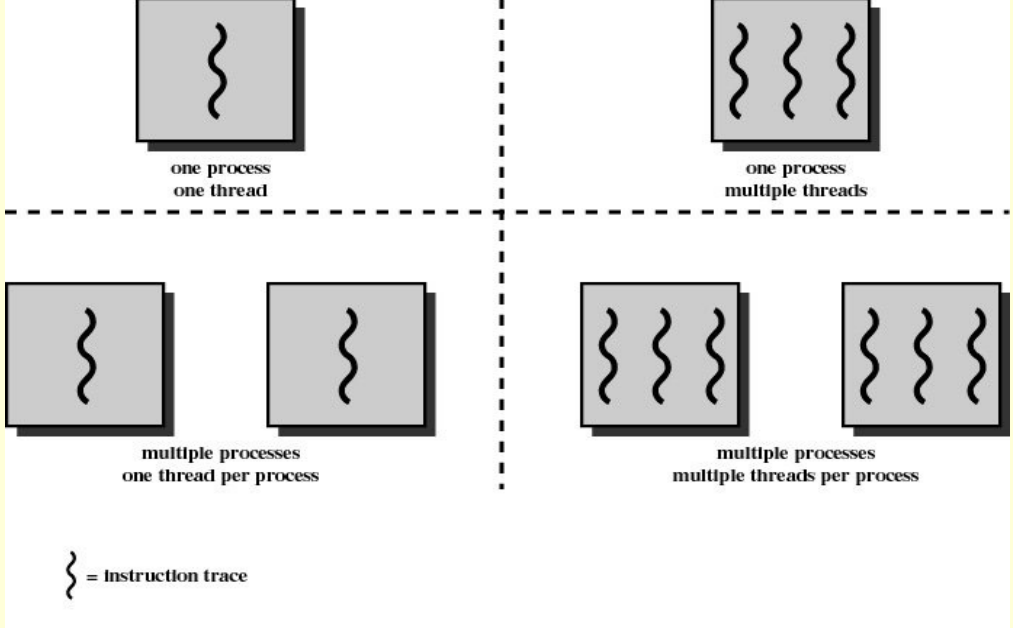
\includegraphics[scale=0.5]{Images/Screenshot 2023-05-23 115150.png
    }
    \caption{Molteplicity process/thread}
    \label{fig:my_label}
\end{figure}

\subsection{Thread}
Thread are created by the programmer or by the OS, this would be for a portion of the code that could be parallelize\footnote{Ex. un ciclo for senza loop-carried dependency}, this need a complication in HW, because every thread need his own Program counter and register file, but not the functional unit of the processor\footnote{ATTENZIONE ALLA DIFFERENZA TRA THREAD HW E THREAD SW}. This allows multiple threads to share the functional unit to improve the throughput of the CPU. The memory address space can be shared too, but we will see that this will need coherence logic.\clearpage
\subsection{Types of multithreading}
\begin{enumerate}
    \item Coarse-grained Multithreading
    \begin{figure}[h!]
        \centering
        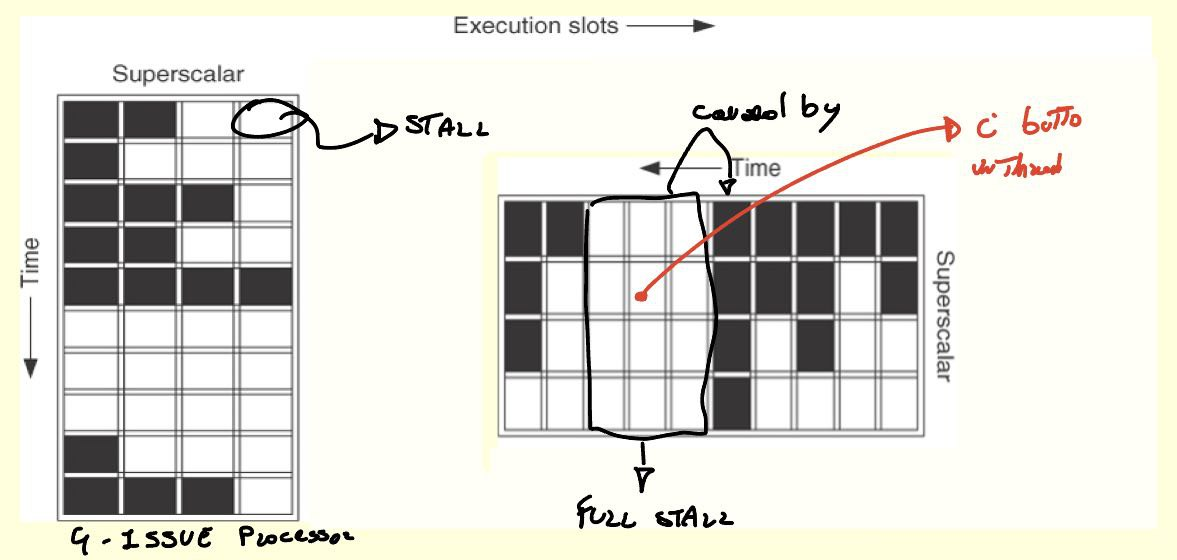
\includegraphics[scale = 0.2]{Images/photo_2023-05-23_12-00-58.jpg}
        \caption{We are putting a new thread while the T1 is full stalled}
        \label{fig:my_label}
    \end{figure}
    This will hide long stall caused by memory miss.
\begin{figure}[h!]
    \centering
    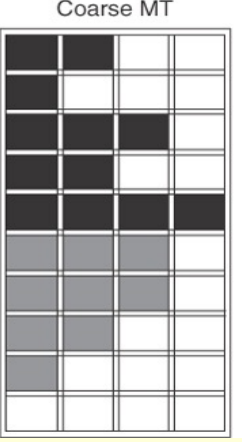
\includegraphics[scale=0.6]{Images/Screenshot 2023-05-23 120634.png}
    \caption{Coarse}
    \label{fig:my_label}
\end{figure}
\item Fine-Grained,  this type of Multithreading check each instruction if one thread is stalled in a round-robin way, skipping stalled thread trying to eliminate empty slots. \begin{figure}[h!]
    \centering
    \includegraphics[scale=0.5]{Images/Screenshot 2023-05-23 121150.png
    \item }
    \caption{Fine-Grained MT}
    \label{fig:my_label}
\end{figure} this is an effective way to hide long-latency event and keep CPU busy.
In this method, we have to discuss the difference between SW Thread and HW Thread.
\begin{itemize}
    \item  SW  Thread, thisispe of thread is managed from the OS with a context switch and is not physically in the core.
    \item HW Thread are physically on the chip and they are not managed from OS
\end{itemize}
So I.E. every HW thread can handle multiple SW threads.
\item Simultaneous Multithreading is the more complex type
\begin{figure}[h!]
    \centering
    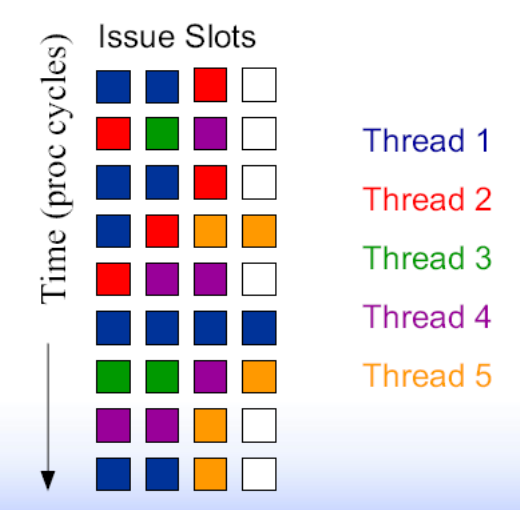
\includegraphics[scale = 0.5]{Images/Screenshot 2023-05-23 122335.png}
    \caption{Simultaneous Threading}
    \label{fig:my_label}
\end{figure}
This technique comes naturally when we use dynamic scheduling and multiple issue processor. With this, we have a sizeable scalable processor that can improve a lot the performance with regards to the other component this improve the performance without improving a lot the power consumption.
\end{enumerate}
\clearpage

\section{Multiprocessor}
Right now many processors are running multi-core solutions, so this topic is very important to understand the state of the art. We are entering \textit{\textbf{MIMD}} architecture, in fact, every processor has its own data and instruction, and every processor could have multithreading or not.
\subsection{Connection of processors}
By increasing the number of processors we can see that will be an increase in cost.
There are 2 main connections:
\begin{enumerate}
    \item Single bus, mostly used with a low number of processors
    \item Interconnection networks, mostly used with a high number of processor
\end{enumerate}
\subsubsection{Single bus multiprocessor}
It's an evolution of \textit{Von Neumann} architecture that contains multiple nodes
\begin{figure}[h!]
    \centering
    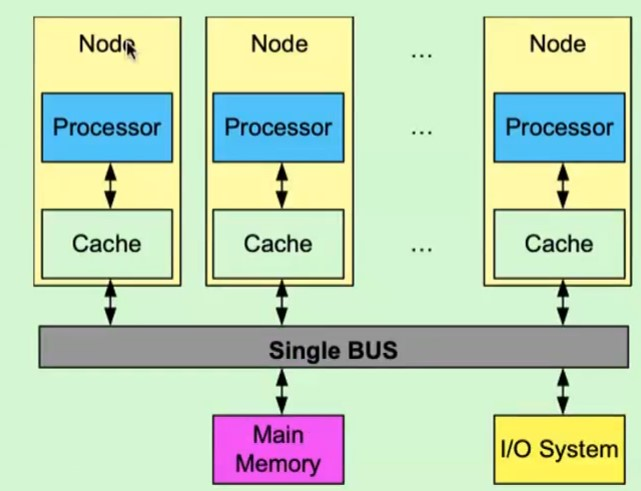
\includegraphics[scale = 0.5]{Images/Screenshot_1.jpg}
    \caption{Single bus}
    \label{fig:enter-label}
\end{figure}
Each node has its own cache and processor.\\
We have a single bus so if one node need to send a communication the bus will be occupied and no more node can communicate in the same bus.
\clearpage
\subsubsection{Network-connected}
In this case, we have a memory attached to the processor and the connection could be a single bus, but in the most of the case we will get a more complex network.
\begin{figure}[h!]
    \centering
    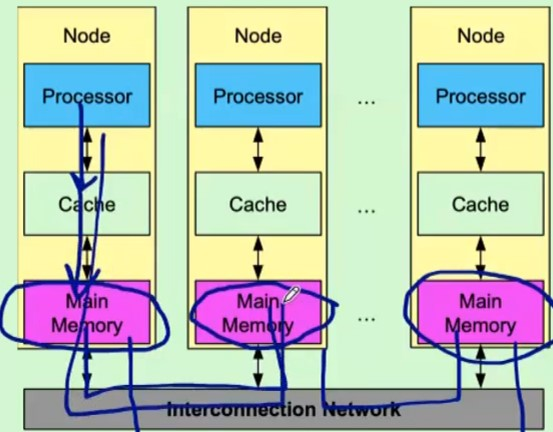
\includegraphics[scale = 0.5]{Images/Screenshot_2.jpg}
    \caption{Network connected}
    \label{fig:enter-label}
\end{figure}
\subsection{Network Topologies}
There are multiple topologies
\begin{itemize}
    \item Single-bus
\begin{figure}[h!]
    \centering
    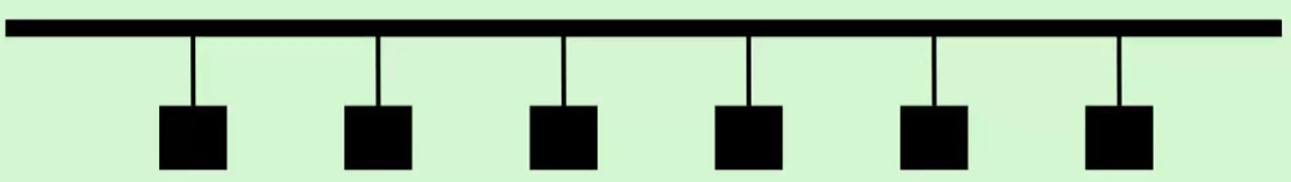
\includegraphics[scale = 0.5]{Images/Screenshot_3.jpg}
    \caption{Single bus topology}
    \label{fig:enter-label}
\end{figure}
\item Ring, this topology can do simultaneous transfers. The communication between nodes needs to pass through intermediate nodes to reach the final destination.
\begin{figure}[h!]
    \centering
    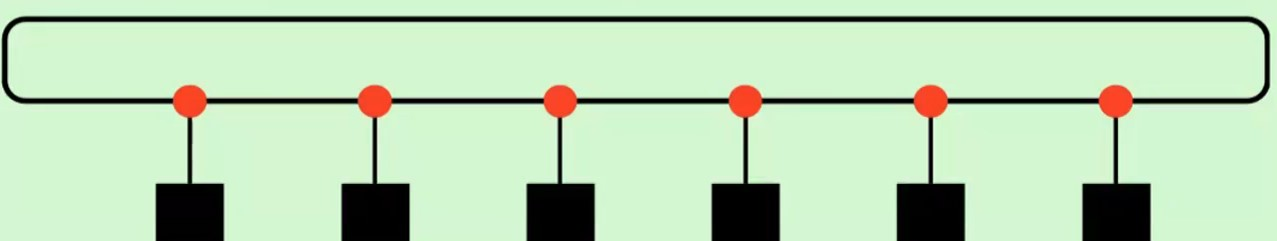
\includegraphics[scale = 0.5]{Images/Screenshot_4.jpg}
    \caption{Ring topology}
    \label{fig:enter-label}
\end{figure}
\end{itemize}
\subsubsection{Network Performance Metrics}
To measure the performance we need  to introduce a formula:\\
$P=$ number of nodes\\
$M=$ number of links\\
$b=$ bandwidth of a single link\\
That in the best case will be:
\begin{equation*}
    M * b
\end{equation*}
so the number of links is multiplied by the bandwidth of each link. But the world unfortunately is not in the best scenario, so we have to consider the worst.
This is calculated by cutting in an half the nodes\footnote{i quadrati neri}
\begin{figure}[h!]
    \centering
    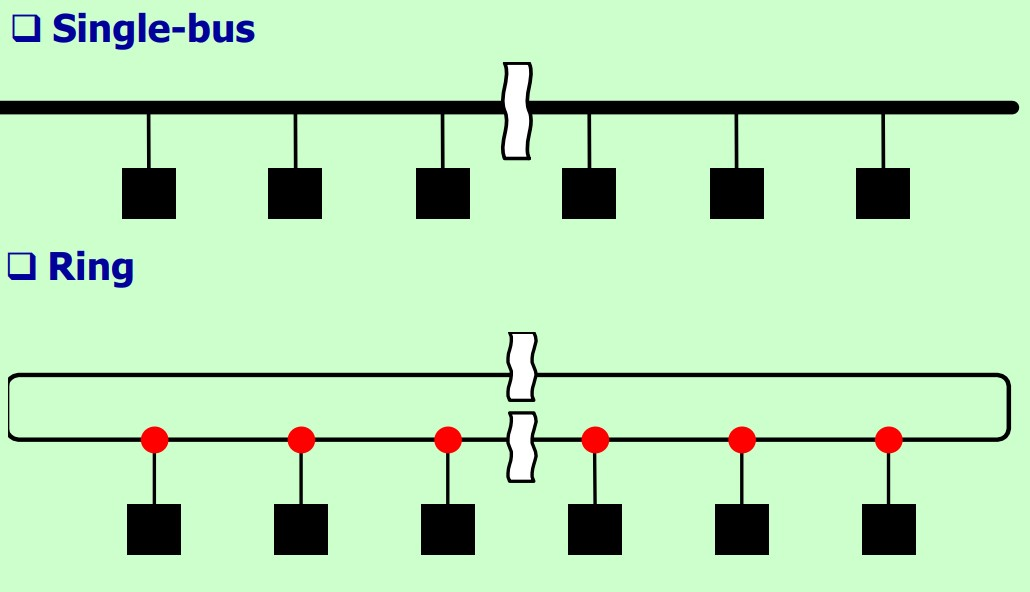
\includegraphics[scale = 0.5]{Images/Screenshot_5.jpg}
    \caption{Bisection}
    \label{fig:enter-label}
\end{figure}
\\So we will get a situation more or less like this\\
\begin{center}
    \begin{tabular}{|l|c|c|}
\hline & $\begin{array}{c}\text { Total } \\
\text { Bandwidth }\end{array}$ & $\begin{array}{c}\text { Bisection } \\
\text { Bandwidth }\end{array}$ \\
\hline Single Bus & $\boldsymbol{b}$ & $\boldsymbol{b}$ \\
\hline Ring & $\boldsymbol{P} \boldsymbol{b}$ & $\boldsymbol{2} \boldsymbol{b}$ \\
\hline
\end{tabular}
\end{center}
Let's now continue the network connection:
\begin{itemize}
    \item Crossbar Network
\begin{figure}[h!]
    \centering
    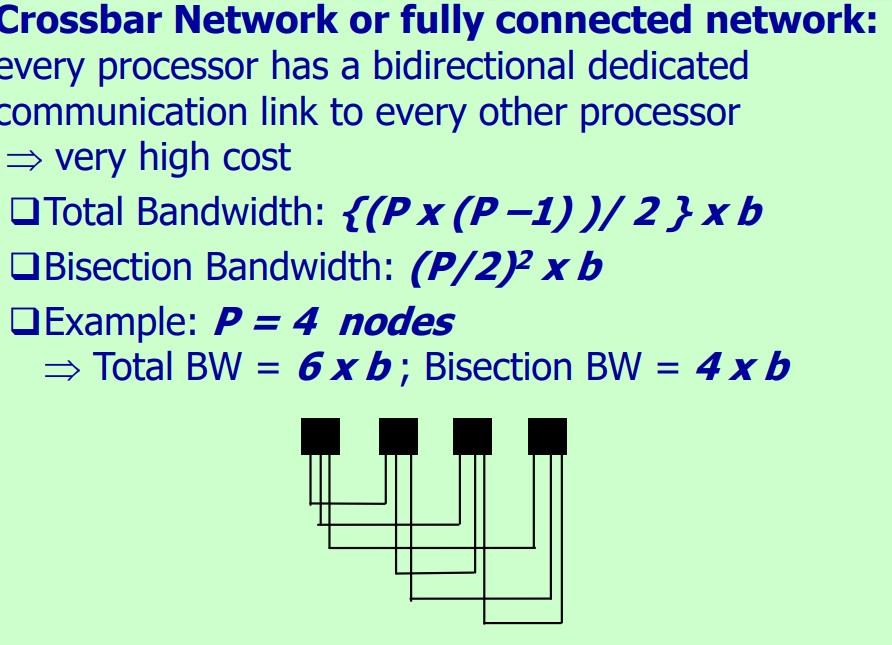
\includegraphics[width=0.5\linewidth]{Images/Screenshot_6.jpg}
    \caption{Crossbar}
    \label{fig:enter-label}
\end{figure}\clearpage
    \item Bidimensional Mesh
\begin{figure}[h!]
    \centering
    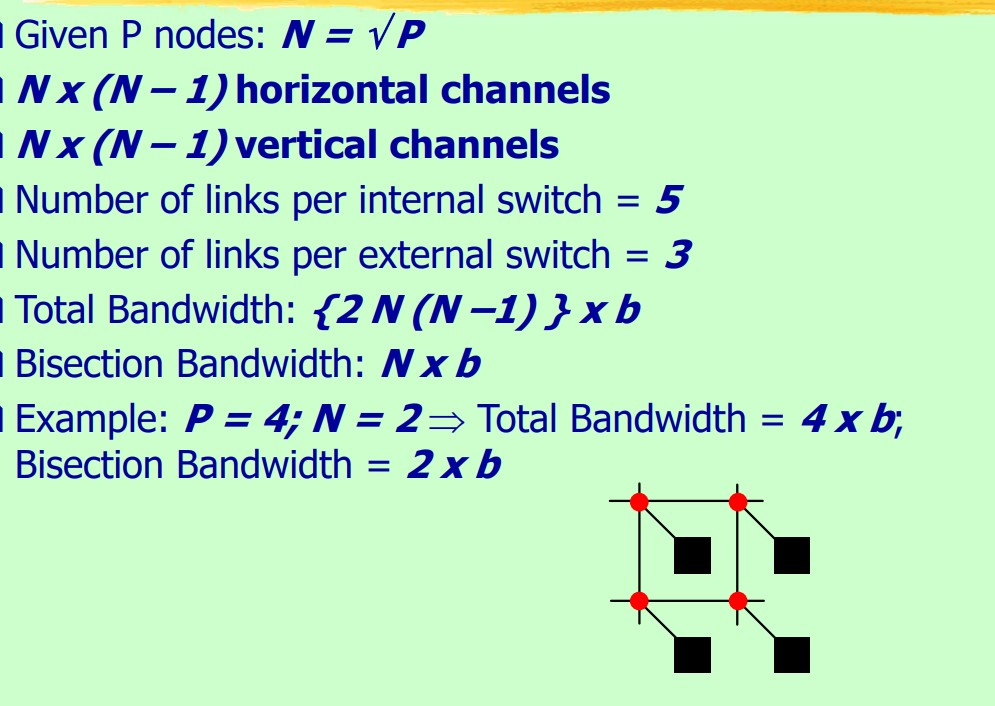
\includegraphics[width=0.5\linewidth]{Images/Screenshot_7.jpg}
    \caption{Mesh}
    \label{fig:enter-label}
\end{figure}
    \item HyperCube
\begin{figure}[h!]
    \centering
    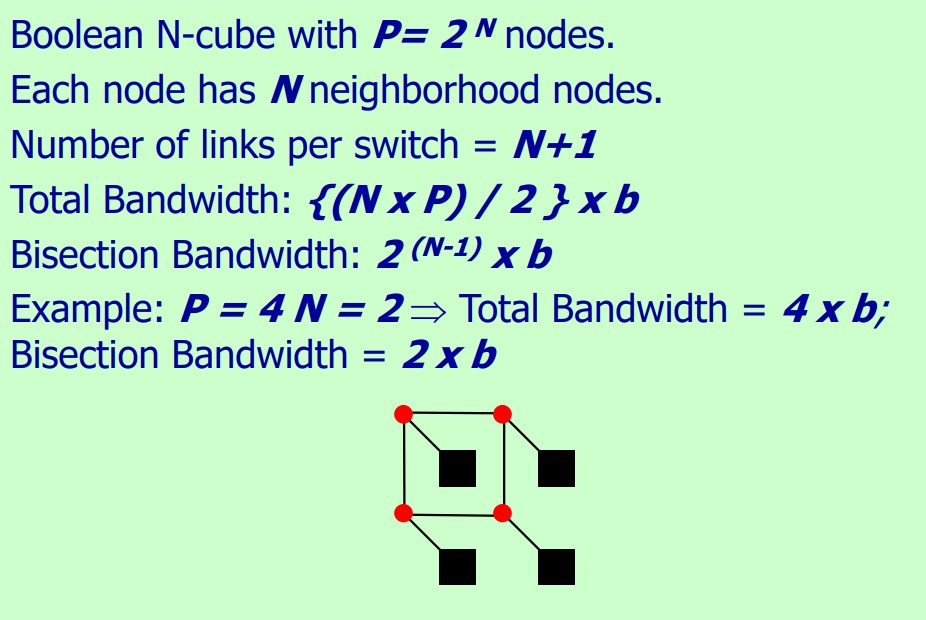
\includegraphics[width=0.5\linewidth]{Images/Screenshot_9.jpg}
    \caption{HyperCube}
    \label{fig:enter-label}
\end{figure}
\end{itemize}
\clearpage\subsection{Shared of Data}
We are in a bivio, we can choos two type with his pros and cons.
\begin{itemize}
    \item Single logically shared address space, with this idea any processor can make a reference to any memory through loads/stores instruction. In this case, one address is the same for every processor in the chip.
\begin{figure}[h!]
        \centering
        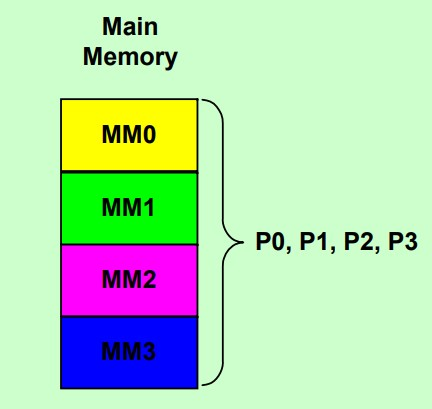
\includegraphics[width=0.25\linewidth]{Images/Screenshot_10.jpg}
        \caption{Single logically shared address}
        \label{fig:enter-label}
    \end{figure}
\\This model imposes the \textit{\textbf{Cache Coherence problem}} among processors.
To be clear shared memory does not mean that there is a single centralized memory, it can be distributed all over the chip in all the processor\footnote{ocio che è una domanda}.\\
It's also called \textit{OpenMPI}.
    \item Multiple address spaces, in this idea every processor has its own bank memory, and the communication among those must be through send/receive message with an \textit{\textbf{Message Passing Architectures}}, the address space is logically disjointed so 2 same addresses in 2 different processors refer to a different memory location.
\begin{figure}[h!]
        \centering
        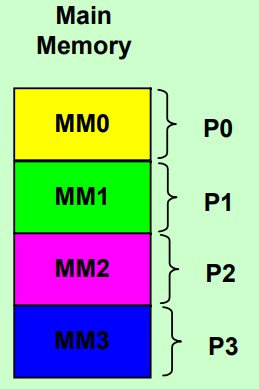
\includegraphics[width=0.25\linewidth]{Images/Screenshot_11.jpg}
        \caption{Multiple Address}
        \label{fig:enter-label}
    \end{figure}
\\This method will not cause any problem with cache coherency.
It's also called \textit{MPI}
\end{itemize}
\textbf{WE ARE LOOKING JUST AT MEMORY AND FROM A LOGICAL POINT OF VIEW NOT THEIR PHYSICAL POINT OF VIEW}\clearpage

\subsection{Physical memory organization}
How is placed this memory?\\
We can have two types of organization
\begin{enumerate}
    \item Centralized Memory (UMA), in this organization the access time to a memory location is \textit{\textbf{uniform}} for all the processors.
\begin{figure}[h!]
        \centering
        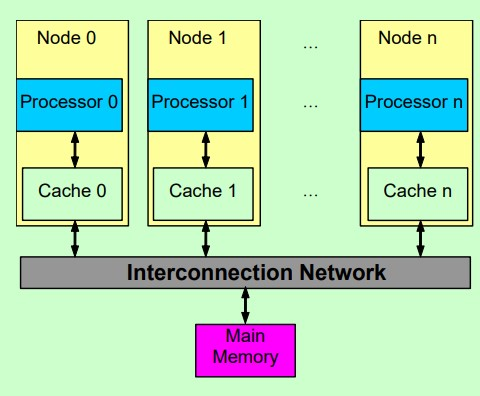
\includegraphics[width=0.5\linewidth]{Screenshot_12.jpg}
        \caption{UMA}
        \label{fig:enter-label}
    \end{figure}
    \item Distributed Memory (NUMA), the memory is physically divided into modules distributed on every single processor, and the memory location access time \textit{\textbf{IS NOT UNIFORM}} for all processors.
\begin{figure}[h!]
        \centering
        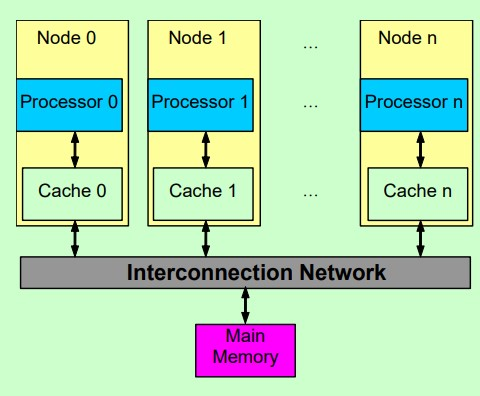
\includegraphics[width=0.5\linewidth]{Screenshot_12.jpg}
        \caption{NUMA}
        \label{fig:enter-label}
    \end{figure}
\end{enumerate}
The concept of address space and the physical memory organization are \textit{orthogonal} to each other, so I can create all 4 options:
\clearpage

\begin{enumerate}
    \item UMA / single address
\begin{figure}[h!]
        \centering
        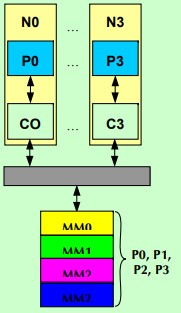
\includegraphics[width=0.12\linewidth]{Screenshot_14.jpg}
        \caption{UMA / single address}
        \label{fig:enter-label}
    \end{figure}
    \item NUMA / Single Address
\begin{figure}[h!]
        \centering
        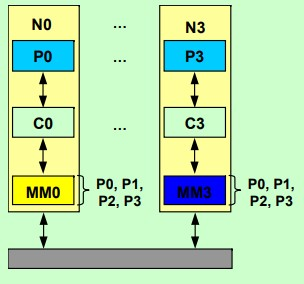
\includegraphics[width=0.20\linewidth]{Screenshot_15.jpg}
        \caption{NUMA / Single Address}
        \label{fig:enter-label}
    \end{figure}
    \item UMA / Multiple address\begin{figure}[h!]
        \centering
        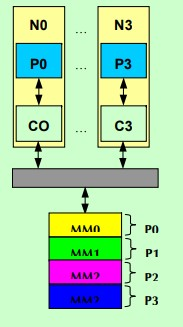
\includegraphics[width=0.15\linewidth]{Screenshot_16.jpg}
        \caption{UMA / Multiple addresses}
        \label{fig:enter-label}
    \end{figure}
    \item NUMA / Multiple address\begin{figure}[h!]
        \centering
        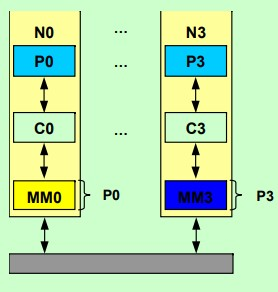
\includegraphics[width=0.20\linewidth]{Screenshot_17.jpg}
        \caption{NUMA / Multiple address}
        \label{fig:enter-label}
    \end{figure}
\end{enumerate}
\clearpage
\subsubsection{Centralized and shared}
Most of the existing multicores are single-chip with a small number of nodes with a single bus and Centralized shared address memory. \\
As we said in the shared address memory we have some problems on cache coherency, try to imagine a solution that will be discussed later.\\
\begin{figure}[h!]
        \centering
        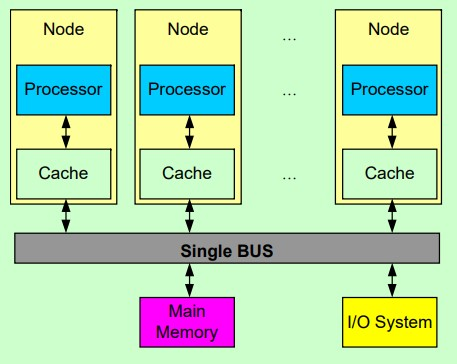
\includegraphics[width=0.5\linewidth]{Screenshot_18.jpg}
        \caption{UMA / Single address}
        \label{fig:enter-label}
    \end{figure}
\\The problem is we have multiple caches, and I've potentially multiple copies of my data, if we are just reading there is no problem, but if someone has a beautiful idea to write?\\
I have a problem keeping coherency to the main memory and the other cache, we already saw a solution with cache and main memory, now we have to expand \textit{Write Through} and \textit{Write Back} to the horizontal problem.
\subsection{Programing a multiprocessor}
When we are very skilled programmers, we think that with a programming language, we can exploit the world, but not every time is like this, in fact, if we are going to program a multiprocessor architecture we need to do a checklist and thinks first about our architecture how is made and after how made our program.\\
In fact, we have to manage a programming model because we will get multiple jobs and programs. We have to understand which type of communication between the node is present so if we have to use a shared address space (OpenMP) or a message passing protocol. In the end, is possible to change the paradigm that uses \textit{GPU or Vector processor}\footnote{ne parliamo dopo}to get a single instruction in multiple data.
\clearpage
\section{Cache Coherency}
This is a problem caused by shared cache in a multiprocessor architecture, we already know how to fix cache coherency in a vertical way\footnote{dalla cache alla main memory}, but now we discuss how to keep it coherence with all the nodes among a chip.\\
When shared data is cached, the corresponding value may be replicated in multiple caches.
While reducing the access latency \textit{(and the relative cost of memory bandwidth)}, this replication provides a reduction of shared data contention read by multiple processors simultaneously
The use of multiple copies of the same data introduces the aforementioned problem of cache coherency.\\
Consider the following sequence of operations performed by a \textit{shared data SIMD} with \(2\) processors:

\begin{figure}[h!]
    \centering
    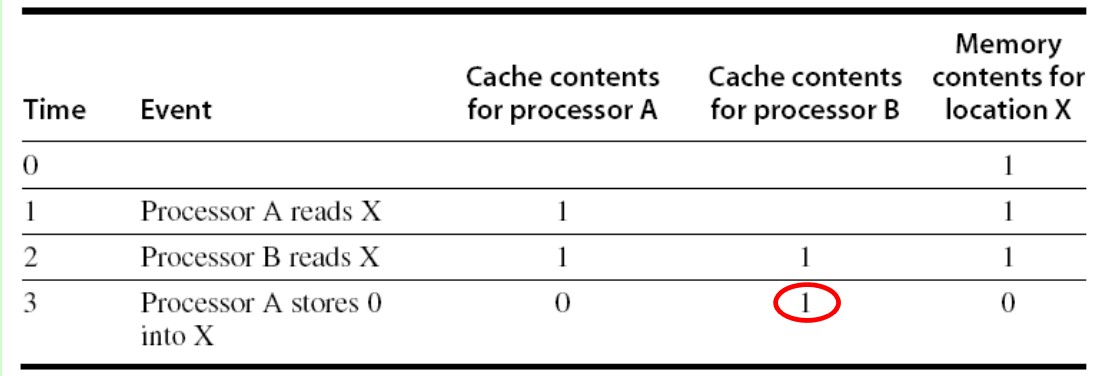
\includegraphics[width=0.5\linewidth]{Images/Screenshot_20.jpg}
    \caption{Cache coherency problem}
    \label{fig:enter-label}
\end{figure}
What does \texttt{B} read?\\
\textbf{The two processors see different values for the same shared variable.}
\\
We need to understand how to keep the coherent and consistent the data, there exist 2 main methods:
\begin{enumerate}
    \item Snooping protocols
    \item Directory based protocols
\end{enumerate}
\subsection{Snooping protocols}

All cache controllers monitor \textit{(or snoop)} the \texttt{BUS} to determine whether they have a copy of the data requested in the block or not.
Every cache that has a copy of the shared data also has a copy of the sharing status of the block, removing the need of keeping a centralized state.

All requests for shared data are sent to all processors.
This solution requires broadcast since the cache controllers must know the sharing status of all the data blocks;
as such, it's particularly suitable for \textbf{Centralized Shared Memory Architectures}, especially for small-scale multiprocessors with single \texttt{BUS}.
\begin{itemize}
  \item The cache controller \textbf{snoops all transactions} on the shared \texttt{BUS}
        \begin{itemize}
          \item the \texttt{BUS} is merely a broadcast medium
        \end{itemize}
  \item If a block contains the \textbf{address tag} of a variable contained in the cache, then:
        \begin{itemize}
          \item the processor must \textit{take action}, either \textbf{invalidating}, \textbf{updating} or \textbf{supplying} the value
          \item the action depends on the \textbf{state} of the block and on the protocol
        \end{itemize}
\end{itemize}

\begin{figure}[h!]
    \centering
    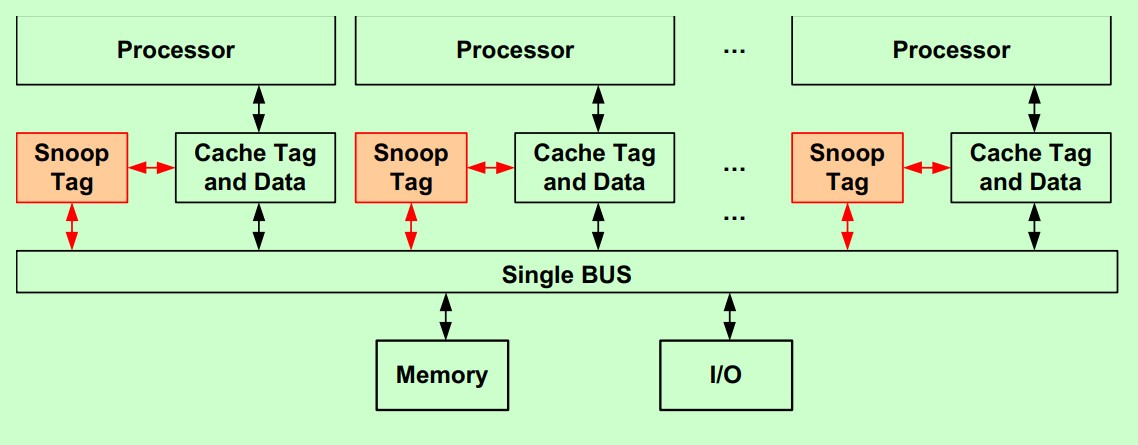
\includegraphics[width=0.5\linewidth]{Images/Screenshot_21.jpg}
    \caption{Snooping architecture}
    \label{fig:enter-label}
\end{figure}

\bigskip
Since every \texttt{BUS} transaction checks the cache address tags, this operation can interfere with the processor operations, causing stalls when the variable is not available in the cache.

To reduce the number of interferences with the processor's accesses to the cache, the tag portion of the address is duplicated for snooping activities.
An extra read port is also added to the address tag portion of the cache.

\bigskip
When a \textbf{miss} happens, the following actions are performed:

\begin{itemize}
  \item In case of a \textbf{write} operation:
        \begin{enumerate}
          \item the address is invalidated in all other caches before the write is performed
          \item this process is called \textbf{Write-Invalidate Protocol}
        \end{enumerate}
  \item In case of a \textbf{read} operation:
        \begin{enumerate}
          \item if a dirty copy is found in some cache, a write-back is performed before the memory is read
          \item this process is called \textbf{Write-Update Protocol} or \textbf{Write-Broadcast Protocol}
        \end{enumerate}
\end{itemize}
\subsubsection{Write-Invalidate Protocol}

The writing processor issues an invalidation signal over the \texttt{BUS} to cause all copies in other caches to be invalidated before changing its local copy:
at this point, it is free to update the local data until another processor asks for it.

All caches on the \texttt{BUS} check to see if they have a copy of the data and if so, they must invalidate the block containing it.
This scheme allows multiple \textbf{readers but} only a \textbf{single writer}: the \texttt{BUS} is used only on the first write to invalidate all other copies while subsequent writes do not result in \texttt{BUS} activity.

\bigskip
Different operations of the protocol:

\begin{itemize}
  \item Basic \textbf{Bus Based} Protocol
        \begin{itemize}
          \item each processor keeps track of cache and state
          \item all transactions over \texttt{BUS} are snooped
        \end{itemize}
  \item Writes \textbf{invalidate} all other caches
        \begin{itemize}
          \item multiple readers can read the same block
          \item a single \texttt{write} invalidates all other copies
        \end{itemize}
  \item Each block in cache has \textbf{two states}
        \begin{itemize}
          \item the state of a block is a \(p\)-vector of states
          \item hardware state bits are associated with blocks that are in the cache
          \item other blocks can be seen as being in \textit{invalid} in that cache
        \end{itemize}
\end{itemize}

Finally, on a \texttt{WRITE} operation, all other copies of the same data are \textbf{invalidated}.
The \texttt{BUS} itself is used to serialize the access to the data, as the \texttt{WRITE} operations cannot complete until exclusive \texttt{BUS} access is obtained.
This protocol is used with \textit{Write-back} and reduces the bus traffic.

\subsubsection{Write-Update Protocol}

In the \textbf{Write-Update protocol}, when a \texttt{WRITE} operation is performed, all the redundant copies of the data are \textbf{invalidated}.
The processor that performs the write also has the duty of updating the main memory and all the other processors' memory, by broadcasting the new value over the \texttt{BUS}.
All caches check if they have a copy of the data and if so, all copies are updated with the new value.
This scheme requires the continuous broadcast of all \texttt{WRITE} operations to the shared data.

This protocol is similar to the \textbf{Write-Through} because all writes are sent over the \texttt{BUS} to update copies of the shared data, but it has the advantage of making the new values appear in caches sooner \textit{(thus reducing the latency)}.
In case of a \texttt{READ} miss, the memory is always up to date.
It's used with \textit{Write-thought}.

\paragraph{Write-through vs Write-back}

The main difference between the two protocols is:

\begin{itemize}
  \item \textbf{Write-through}: the memory is always up to date
  \item \textbf{Write-back}: the caches must be snooped into until the most recent copy is found
\end{itemize}

The write-through protocol is simple, as every \texttt{WRITE} operation is observable:
each one of them goes on the \texttt{BUS}, and as such only one \texttt{WRITE} can take place at a time in any processor.
As a downside, it uses a lot of bandwidth.

\subsubsection{Invalidate vs Update}

Before choosing one of the two protocols, a basic question on the program behaviour must be asked:

\indentquote{Is a block written by one processor later read by others before it is overwritten?}

Then, the two protocols can be compared:

\begin{itemize}
  \item \textbf{Invalidate}
        \begin{itemize}
          \item[\cmark] yes: readers will take a miss
          \item[\xmark] no: multiple writes can be performed without added traffic and old copies will be cleared out
        \end{itemize}
  \item \textbf{Update}
        \begin{itemize}
          \item[\cmark] yes: misses on later references will be avoided
          \item[\xmark] no: multiple useless updates will be broadcast over the \texttt{BUS}
        \end{itemize}
\end{itemize}

In the same way, most commercial cache-based multiprocessors use:

\begin{itemize}
  \item \textbf{Write-Back Caches} to reduce \texttt{BUS} traffic, allowing more processors on a single \texttt{BUS}
  \item \textbf{Write-Invalidate Protocol} to preserve \texttt{BUS} bandwidth
\end{itemize}

\paragraph{Cache State Transition Diagram}

This transition diagram \textit{(represented in Figure~\ref{subfig:MSI-state-transition-diagram})} is applicable to the \textbf{MSI Protocol} \textit{(Modified, Shared, Invalid)}.
Each cache line has state bits, relative to the state of the data.

\begin{figure}[htbp]
  \bigskip
  \centering
  \begin{subfigure}[]{\textwidth}
    \centering
    \begin{tikzpicture}[auto, node distance=3cm, >=Triangle]
      \node [state, initial, initial above, initial text={write miss},  minimum size=1cm](M) {\texttt{M}};
      \node [state, minimum size=1cm, below=of M](I) {\texttt{I}};
      \node [state, initial, initial below, initial text={read miss}, minimum size=1cm, below=of M, left=of I](S) {\texttt{S}};

      \path[->, thick]
      (M) edge [loop right] node {read or write} ()
      (S) edge [loop left] node {read} ()
      (M) edge [bend left] node {write} (I)
      (S) edge [bend right] node {write} (I)
      (M) edge [bend left] node {read} (S)
      (S) edge [bend left] node {write} (M);
    \end{tikzpicture}

    \caption{State Transition Diagram}
    \label{subfig:MSI-state-transition-diagram}
    \bigskip
  \end{subfigure}
  \begin{subfigure}[]{\textwidth}
    \centering
    \tikzfig[01]{image-51.tikz}
    \caption{Structure of a cache line}
    \label{subfig:MSI-cache-line}
  \end{subfigure}
  \caption{\textit{MSI} Protocol Implementation}
  \label{fig:MSI-protocol}
\end{figure}
\clearpage
\subsubsection{MESI Protocol}

The basic \textit{MSI protocol} is not completely suitable to be applied to the real world, since it has a few limitations:

\begin{itemize}
  \item Operations are not \textbf{atomic}
        \begin{itemize}
          \item \textit{deadlocks} and \textit{race conditions} may be introduced
          \item \textbf{solution}: the processor sends invalidate can hold \texttt{BUS} until other processors receive the message
        \end{itemize}
  \item The system is \textbf{hard to extend}
        \begin{itemize}
          \item \textbf{solution}: add an exclusive state to indicate a clean block in only one cache \textit{(MESI Protocol)}
        \end{itemize}
\end{itemize}

\bigskip
A modified version of the \textit{MSI} protocol is the \textit{MESI} protocol.
It implements the Write-Invalidate protocol, with the additional \textbf{shared} state.

Each cache block can then be in one out of \(4\) states:

\begin{enumerate}
  \item \textbf{Modified}: the block is dirty and cannot be shared, the cache has the only copy and it's writeable
  \item \textbf{Exclusive}: the block is clean and the only copy is in the cache
  \item \textbf{Shared}: the block is clean and other copies of the block are in the cache
  \item \textbf{Invalid}: the cache contains invalid data
\end{enumerate}

The \textbf{exclusive} state distinguishes between \textbf{exclusive} \textit{(writable)} and \textbf{owned} \textit{(written)} states.

To support this protocol, all cache controllers snoop on a special \texttt{BUS} called \texttt{BusRd}.
The issuer chooses between the \textbf{shared} and \textbf{exclusive} states, and the \texttt{BUS} is used to send the message to the other caches.

Characteristics of the states:

\begin{itemize}
  \item In both \textbf{shared} and \textbf{exclusive} states the memory has an up-to-date version of the data
  \item A write to an \textbf{exclusive} block does not require sending the invalidation signal on the \texttt{BUS}, since no other copies of the block are in the cache
  \item A write to a \textbf{shared} block implies the invalidation of the other copies of the block in the cache
\end{itemize}

\bigskip



% I am really really really sorry for this abomination
\begin{table}[htbp]
  \centering
  \scalebox{0.6}{
    \rotatebox{0}{
      \begin{tblr}{colspec={r|c|c|c|c}}
        \(\Rsh\)                               & \textit{Modified} & \textit{Exclusive}              & \textit{Shared}                 & \textit{Invalid}                                                                                                                                                                                                                  \\
        \hline
        \textit{Line valid?}                   & \colorcmark       & \colorcmark                     & \colorcmark                     & \colorxmark                                                                                                                                                                                                                       \\
        \textit{Copy in memory}                & has to be updated & valid                           & valid                           & invalid                                                                                                                                                                                                                           \\
        \textit{Other copies in other caches}? & \colorxmark       & \colorxmark                     & maybe                           & \(-\)                                                                                                                                                                                                                             \\
        \textit{Can be written?}               & \colorcmark       & \colorcmark                     & \colorxmark                     & \colorcmark                                                                                                                                                                                                                       \\
        \textit{Can be read?}                  & \colorcmark       & \colorcmark                     & \colorcmark                     & \colorxmark                                                                                                                                                                                                                       \\
        \textit{On read}                       & nothing happens   & nothing happens                 & nothing happens                 & \(\begin{cases}\text{transition to} \textit{ Exclusive } & \text{if data \textbf{is not} on other caches} \\ \text{transition to} \textit{ Shared } &\text{if data \textbf{is} on other caches}\end{cases} \) \\
        \textit{On write}                      & nothing happens   & transition to \textit{Modified} & transition to \textit{Modified} & transition to \textit{Modified}, other copies transition to \textit{Invalidate}                                                                                                                                                   \\
      \end{tblr}
    }
  }
  \caption{State of cache lines with \textit{MESI} Protocol}
  \label{tab:MESI-cache-line}
\end{table}

\begin{figure}[htbp]
  \bigskip
  \centering
  \begin{subfigure}{\textwidth}
    \centering
    \begin{tikzpicture}[auto, node distance=4cm, >=Triangle]
      \node [state, initial, initial left, initial text={\texttt{WRITE} miss},  minimum size=1cm](M) {\texttt{M}};
      \node [state, initial, initial right, initial text={\texttt{READ} miss}, minimum size=1cm, right=of M](E) {\texttt{E}};
      \node [state, initial, initial left, initial text={\texttt{READ} miss}, minimum size=1cm, below=of M](S) {\texttt{S}};
      \node [state, minimum size=1cm, below=of E](I) {\texttt{I}};

      \path[->, thick]
      (M) edge [loop above] node {read or write} ()
      (E) edge [loop above] node {read} ()
      (S) edge [loop below] node {read} ()
      (M) edge [bend right, below, sloped] node {\shortstack{other processors read \\ \texttt{P} writes back}} (S)
      (S) edge [below, sloped] node {intent to write} (M)
      (S) edge [below, sloped] node {\shortstack{other processors\\intent to write}} (I)
      (E) edge [above, sloped] node {\shortstack{other processors\\intent to write}} (I)
      (E) edge [above, sloped] node {write} (M)
      (M) edge [above, sloped] node {\footnotesize\shortstack[l]{other processors intent to write\\write back}} (I)
      (E) edge [above, sloped, pos=0.75] node {\footnotesize other processors read} (S);
    \end{tikzpicture}

    \caption{State Transition Diagram}
    \label{subfig:MESI-state-transition-diagram}
    \bigskip
  \end{subfigure}

  \begin{subfigure}{\textwidth}
    \centering
    \tikzfig[1]{image-53.tikz}
    \caption{Structure of a cache line}
    \label{subfig:MESI-cache-line}
  \end{subfigure}
  \caption{\textit{MESI} Protocol Implementation}
  \label{fig:MESI-protocol}
\end{figure}
\clearpage
\subsection{Directory based protocol}
Here the sharing state of a block of physical memory is kept in just one location called \textit{Directory}. Each entry in the directory is associated to each block in the main memory.
This protocol is mainly used in \textit{\textbf{Distribute shared-memory}} architecture, where the directory is distributed on the nodes to avoid bottleneck.\\
This does not mean that if you use \textit{\textbf{Centralized shared-memory}} architecture you cannot use this protocol.\\
There is an overall mapping of each memory block address to each node, so everyone will know the home node, the node where reside the memory block, and the directory\footnote{dopo ne parliamo}.\\
Everyone in the system knows who refers if need a specific block.
Because is a distributed protocol it will use the Message Passing Protocol paradigm, so the protocol is based on send/receive instruction and this will improve the scalability of the system.
\begin{figure}[h!]
    \centering
    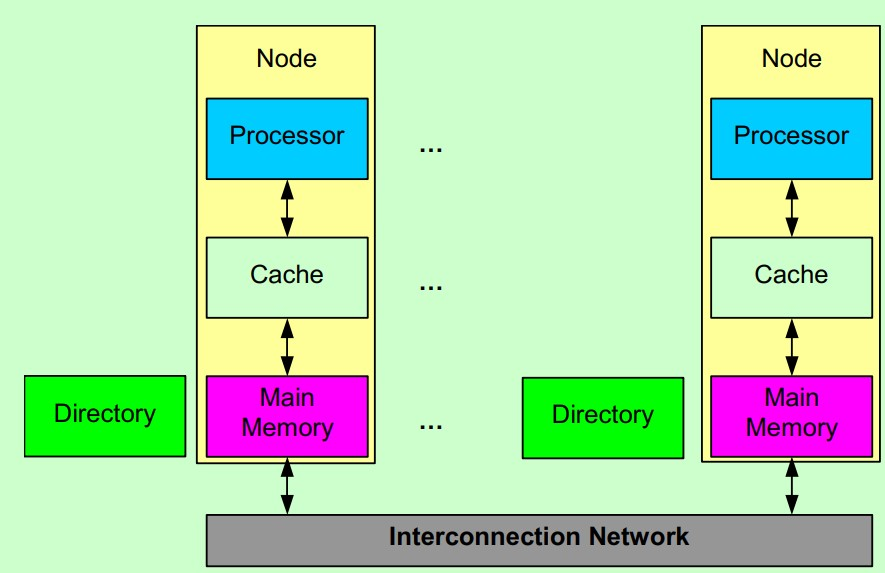
\includegraphics[width=0.5\linewidth]{Images/Screenshot_25.jpg}
    \caption{Directory Based protocol}
    \label{fig:enter-label}
\end{figure}
\subsubsection{Directory}
The directory is the part of the protocol that contains the state and the information of the cache block.
The state of a directory could be:
\begin{itemize}
    \item Uncached, that means nobody has fetched this data
    \item Shared, there are one or more copies around the chip. How holds the copy is determined by the sharer bit, a series of bit that holds a flag that says \textit{\textbf{"This node has this block updated"}}
    \item Modified, there is only one copy around the chip, and the owner, who modified the block, is specified in the sharer bit
\end{itemize}
\begin{figure}[h!]
    \centering
    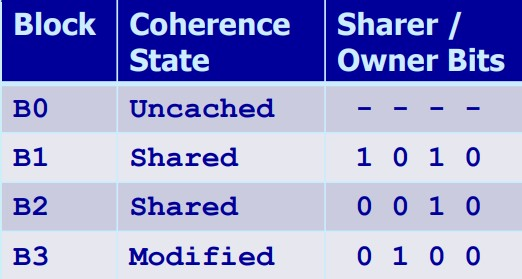
\includegraphics[width=0.5\linewidth]{Images/Screenshot_26.jpg}
    \caption{In this picture we can see what's explained before.}
    \label{fig:state}
\end{figure}
\clearpage\paragraph{Types of Nodes}
There are 3 types of nodes:
\begin{itemize}
    \item Home Node, is the one that holds the memory location.
    \item Local Node, where a request came from.
    \item Remote Node, where there is a copy of the cache block.
\end{itemize}
The \textit{Local Node} can be \textit{Home Node} and vice-versa, but this will be an intranode\footnote{Su se stessa} transaction.\\
The \textit{Remote Node} can be the \textit{Home Node} and vice-versa.\\
The \textit{Local Node} and the \textit{Remote Node} \textbf{MUST BE DIFFERENT}.
\subsubsection{How do they talk to each other?}
As mentioned before they talk with the message, but suppose we are referring to figure \ref{fig:state} and we are \textit{Node2} we want to read \textit{B3}, what we are supposed to do?\\
We must contact the \textit{Home node}, by sending a specific message and he will handle all the stuff.
\paragraph{Type of Message}
\begin{figure}[h!]
    \centering
    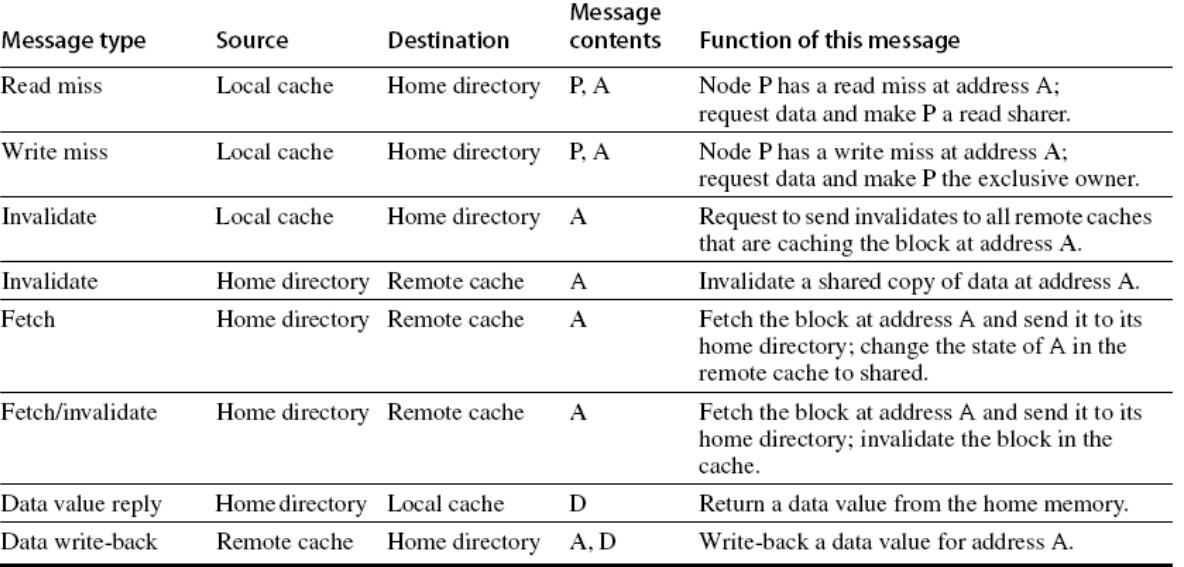
\includegraphics[width=0.5\linewidth]{Images/Screenshot_27.jpg}
    \caption{All types of message}
    \label{fig:enter-label}
\end{figure}
\paragraph{Uncached}
When a directory block is in the uncached block we can only have a miss, no matter if we write or read.\\
So in this case we will send an \textit{Write/Read Miss} from Local to Home, and it should answer with a \textit{Data Value Reply}.

\begin{center}
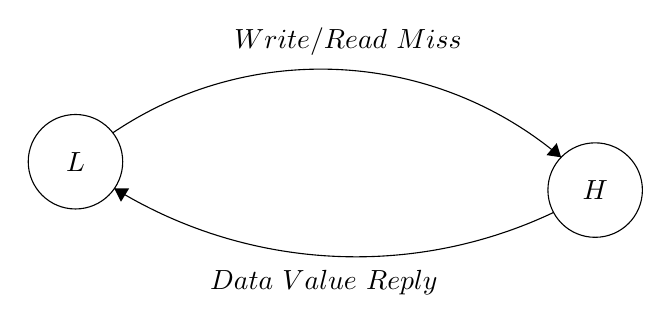
\begin{tikzpicture}[scale=0.2]
\tikzstyle{every node}+=[inner sep=0pt]
\draw [black] (20.5,-15.6) circle (3);
\draw (20.5,-15.6) node {$L$};
\draw [black] (53.5,-17.4) circle (3);
\draw (53.5,-17.4) node {$H$};
\draw [black] (22.872,-13.766) arc (124.06473:49.69101:23.587);
\fill [black] (51.34,-15.32) -- (51.06,-14.42) -- (50.41,-15.18);
\draw (37.81,-8.88) node [above] {$Write/Read\mbox{ }Miss$};
\draw [black] (50.859,-18.82) arc (-64.66222:-121.58204:29.304);
\fill [black] (22.97,-17.3) -- (23.39,-18.14) -- (23.91,-17.29);
\draw (36.27,-22.48) node [below] {$Data\mbox{ }Value\mbox{ }Reply$};
\end{tikzpicture}
\end{center}
\begin{center}
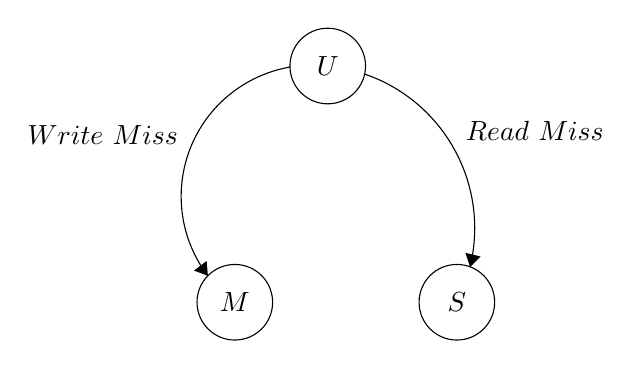
\begin{tikzpicture}[scale=0.2]
\tikzstyle{every node}+=[inner sep=0pt]
\draw [black] (18.5,-2.6) circle (2.4);
\draw (18.5,-2.6) node {$U$};
\draw [black] (26.7,-17.6) circle (2.4);
\draw (26.7,-17.6) node {$S$};
\draw [black] (12.6,-17.6) circle (2.4);
\draw (12.6,-17.6) node {$M$};
\draw [black] (10.894,-15.924) arc (-142.73983:-260.20291:8.335);
\fill [black] (10.89,-15.92) -- (10.81,-14.98) -- (10.01,-15.59);
\draw (9.02,-6.96) node [left] {$Write\mbox{ }Miss$};
\draw [black] (20.84,-3.109) arc (71.09056:-13.76265:10.344);
\fill [black] (27.54,-15.36) -- (28.21,-14.7) -- (27.24,-14.46);
\draw (27.24,-6.75) node [right] {$Read\mbox{ }Miss$};
\end{tikzpicture}
\end{center}
\clearpage
\paragraph{Shared}
In this case, there will be a difference between read and write.\\
If we perform a read miss we will get an data value reply from \textit{Home Node}
\begin{center}
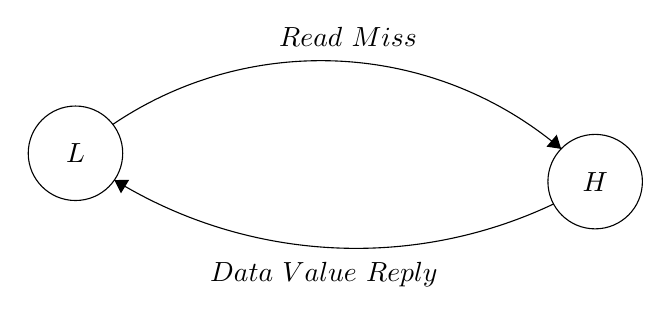
\begin{tikzpicture}[scale=0.2]
\tikzstyle{every node}+=[inner sep=0pt]
\draw [black] (20.5,-15.6) circle (3);
\draw (20.5,-15.6) node {$L$};
\draw [black] (53.5,-17.4) circle (3);
\draw (53.5,-17.4) node {$H$};
\draw [black] (22.872,-13.766) arc (124.06473:49.69101:23.587);
\fill [black] (51.34,-15.32) -- (51.06,-14.42) -- (50.41,-15.18);
\draw (37.81,-8.88) node [above] {$Read\mbox{ }Miss$};
\draw [black] (50.859,-18.82) arc (-64.66222:-121.58204:29.304);
\fill [black] (22.97,-17.3) -- (23.39,-18.14) -- (23.91,-17.29);
\draw (36.27,-22.48) node [below] {$Data\mbox{ }Value\mbox{ }Reply$};
\end{tikzpicture}
\end{center}
And the state will not be modified.\\
The symphony changes if we perform a \textit{Write Miss}, in fact, the home node must invalidate all the copies in the system.
\begin{center}
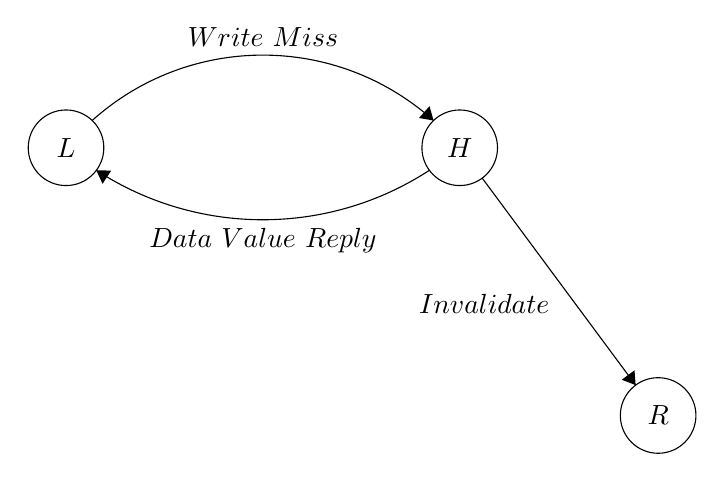
\begin{tikzpicture}[scale=0.2]
\tikzstyle{every node}+=[inner sep=0pt]
\draw [black] (2.6,-8.3) circle (2.4);
\draw (2.6,-8.3) node {$L$};
\draw [black] (27.6,-8.3) circle (2.4);
\draw (27.6,-8.3) node {$H$};
\draw [black] (40.2,-25.3) circle (2.4);
\draw (40.2,-25.3) node {$R$};
\draw [black] (4.26,-6.57) arc (131.94619:48.05381:16.217);
\fill [black] (25.94,-6.57) -- (25.68,-5.66) -- (25.01,-6.41);
\draw (15.1,-1.91) node [above] {$Write\mbox{ }Miss$};
\draw [black] (29.03,-10.23) -- (38.77,-23.37);
\fill [black] (38.77,-23.37) -- (38.7,-22.43) -- (37.89,-23.03);
\draw (33.32,-18.19) node [left] {$Invalidate$};
\draw [black] (25.675,-9.731) arc (-56.91604:-123.08396:19.373);
\fill [black] (4.52,-9.73) -- (4.92,-10.59) -- (5.47,-9.75);
\draw (15.1,-13.37) node [below] {$Data\mbox{ }Value\mbox{ }Reply$};
\end{tikzpicture}
\end{center}
And the state will change as follows:

\begin{center}
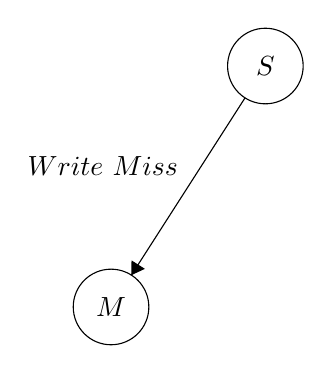
\begin{tikzpicture}[scale=0.2]
\tikzstyle{every node}+=[inner sep=0pt]
\draw [black] (14.6,-2.6) circle (2.4);
\draw (14.6,-2.6) node {$S$};
\draw [black] (4.8,-17.9) circle (2.4);
\draw (4.8,-17.9) node {$M$};
\draw [black] (13.31,-4.62) -- (6.09,-15.88);
\fill [black] (6.09,-15.88) -- (6.95,-15.48) -- (6.1,-14.94);
\draw (9.08,-8.94) node [left] {$Write\mbox{ }Miss$};
\end{tikzpicture}
\end{center}
\paragraph{Modified}
In this state, we have modified data so every time someone performs an action on this data the Home node must fetch it. But there is still a difference between write and read. In fact the first will also invalidate after the fetch.
\begin{center}
\begin{tikzpicture}[scale=0.2]
\tikzstyle{every node}+=[inner sep=0pt]
\draw [black] (2.6,-9.3) circle (2.4);
\draw (2.6,-9.3) node {$L$};
\draw [black] (27.8,-10.2) circle (2.4);
\draw (27.8,-10.2) node {$H$};
\draw [black] (48,-10.2) circle (2.4);
\draw (48,-10.2) node {$R$};
\draw [black] (4.084,-7.417) arc (137.10152:38.80766:14.797);
\fill [black] (26.45,-8.22) -- (26.34,-7.28) -- (25.56,-7.91);
\draw (15.68,-1.9) node [above] {$(1)\mbox{ }Write/Read\mbox{ }Miss$};
\draw [black] (47.225,-12.466) arc (-25.53262:-154.46738:10.334);
\fill [black] (47.23,-12.47) -- (46.43,-12.97) -- (47.33,-13.4);
\draw (37.9,-18.85) node [below] {$(2)\mbox{ }Fetch/Fetch&Invalidate$};
\draw [black] (29.049,-8.156) arc (142.41935:37.58065:11.169);
\fill [black] (29.05,-8.16) -- (29.93,-7.83) -- (29.14,-7.22);
\draw (37.9,-3.3) node [above] {$(3)\mbox{ }Write\mbox{ }Back$};
\draw [black] (26.301,-12.071) arc (-43.32215:-140.76867:14.872);
\fill [black] (3.96,-11.27) -- (4.08,-12.21) -- (4.85,-11.58);
\draw (14.71,-17.54) node [below] {$(4)\mbox{ }Data\mbox{ }Value\mbox{ }Reply$};
\end{tikzpicture}
\end{center}

\paragraph{Final FSM of the directory based}
\begin{center}
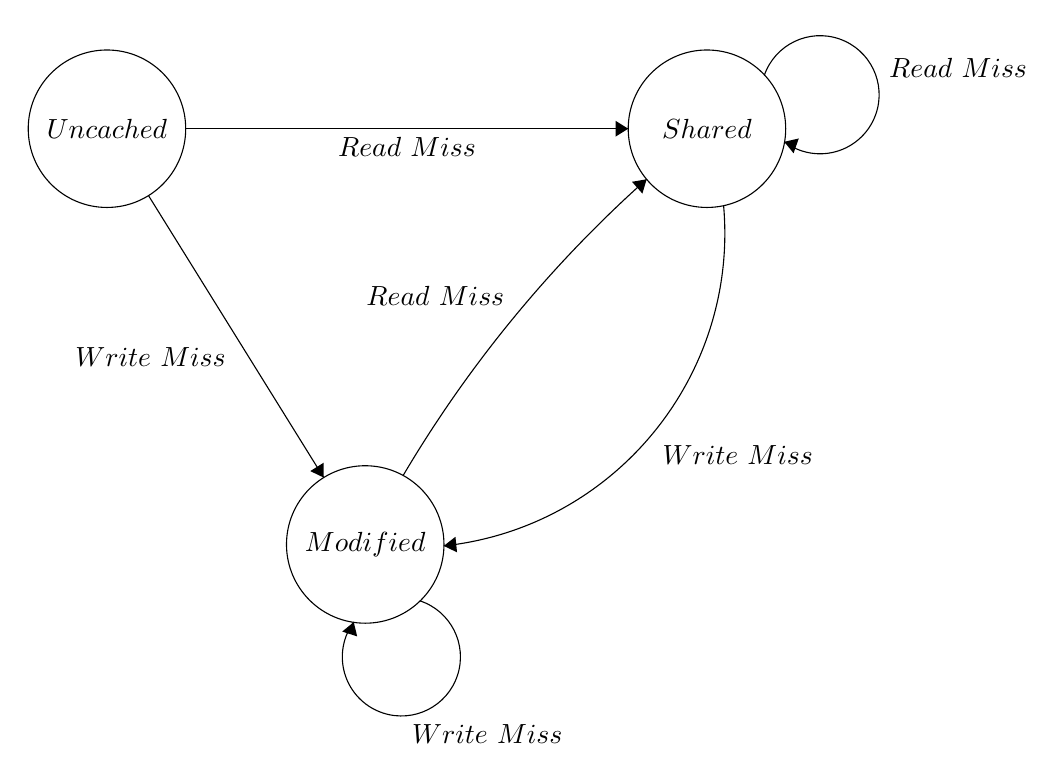
\begin{tikzpicture}[scale=0.2]
\tikzstyle{every node}+=[inner sep=0pt]
\draw [black] (5.2,-6.2) circle (5);
\draw (5.2,-6.2) node {$Uncached$};
\draw [black] (43.3,-6.2) circle (5);
\draw (43.3,-6.2) node {$Shared$};
\draw [black] (21.6,-32.6) circle (5);
\draw (21.6,-32.6) node {$Modified$};
\draw [black] (10.2,-6.2) -- (38.3,-6.2);
\fill [black] (38.3,-6.2) -- (37.5,-5.7) -- (37.5,-6.7);
\draw (24.25,-6.7) node [below] {$Read\mbox{ }Miss$};
\draw [black] (46.943,-2.804) arc (160.72332:-127.27668:3.75);
\draw (54.84,-2.36) node [right] {$Read\mbox{ }Miss$};
\fill [black] (48.21,-7.03) -- (48.8,-7.76) -- (49.13,-6.82);
\draw [black] (44.356,-11.074) arc (5.05671:-83.89505:19.972);
\fill [black] (26.59,-32.69) -- (27.43,-33.1) -- (27.33,-32.11);
\draw (40.45,-26.95) node [right] {$Write\mbox{ }Miss$};
\draw [black] (24.007,-28.219) arc (149.407:131.75466:79.339);
\fill [black] (39.47,-9.41) -- (38.54,-9.57) -- (39.2,-10.32);
\draw (30.46,-16.79) node [left] {$Read\mbox{ }Miss$};
\draw [black] (25.065,-36.177) arc (71.81889:-216.18111:3.75);
\draw (29.35,-44.01) node [below] {$Write\mbox{ }Miss$};
\fill [black] (20.87,-37.53) -- (20.14,-38.13) -- (21.09,-38.44);
\draw [black] (7.84,-10.45) -- (18.96,-28.35);
\fill [black] (18.96,-28.35) -- (18.96,-27.41) -- (18.11,-27.94);
\draw (12.77,-20.69) node [left] {$Write\mbox{ }Miss$};
\end{tikzpicture}
\end{center}
\clearpage
\section{Vector Processor}
\textbf{Vector processors} have high-level operations that work on linear arrays of number \textit{(also called vectors)}.
A language that can handle vectors \textit{(and not scalar values)} is needed as well.\\
\bigskip
\textit{Basic idea}:
\begin{itemize}
  \item \textbf{Read} sets of data elements into \textit{vector registers}
  \item \textbf{Operate} on those registers
  \item \textbf{Disperse} the results back into memory
  \item Adaptable to \textbf{different data types}
        \begin{itemize}
          \item a vector size can be seen as \(64\) 64-bit elements, \(32\) 128-bit elements, \ldots
This is because we will adapt our architecture to the application's size.
        \end{itemize}
  \item A single instruction operates on \textbf{vectors} of data
        \begin{itemize}
          \item the result involves many registers to register operations
          \item used to hide memory latency
          \item leverages memory bandwidth
        \end{itemize}
\end{itemize}
\bigskip
In this type of architecture, we have a radical change, now we have a controller of the architecture, but the processing element is distributed and they can access some data:
\begin{figure}[h!]
    \centering
    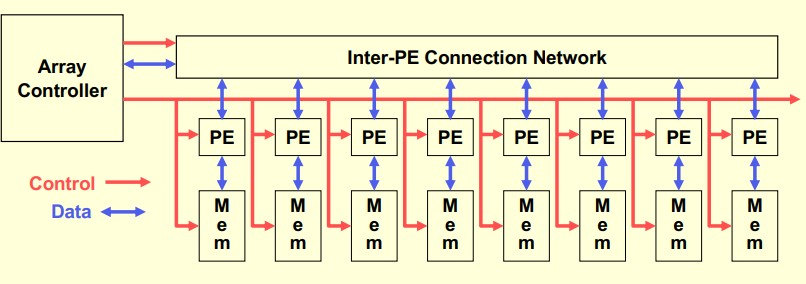
\includegraphics[width=0.5\linewidth]{Images/Screenshot_29.jpg}
    \caption{SIMD Architecture}
    \label{fig:enter-label}
\end{figure}
 The use of this paradigm is very useful for exploiting significant Data level parallelism.\\
 \subsection{How is made a Vector processor}
 A vector processor is made by:
 \begin{itemize}
     \item Load/store Architecture
     \item Vector Register
     \item Vector Instruction
     \item Hardwired Control
     \item Highly Pipelined Functional Unite
     \item Interleaved Memory System
     \item No Data Cache
     \item No Virtual Memory
 \end{itemize}
 From this is created the \textit{\textbf{VMIPS}} that will be discussed later.\\
 The idea is to combine multiple scalar models at one time
\begin{figure}[htbp]
  \bigskip
  \centering
  \begin{subfigure}[b]{0.495\textwidth}
    \centering
    \tikzfig[1]{image-58.tikz}
    \caption{Scalar model, \(1\) operation at a time}
    \label{subfig:vector-model}
  \end{subfigure}
  \begin{subfigure}[b]{0.495\textwidth}
    \centering
    \tikzfig[1]{image-59.tikz}
    \caption{Vector mode, \(n\) operations at a time}
    \label{subfig:scalar-model}
  \end{subfigure}
  \caption{Comparison of scalar and vector models}
  \label{fig:comparison-of-models}
  \bigskip
\end{figure}
To perform this idea we must be sure that every element is independent of each other\footnote{NO LOOP CARRIED}.\\
The use of this paradigm is very useful for exploiting significant \textbf{Data level parallelism} with more energy efficient than \textbf{MIMD.}
\subsection{Vector processing}

A vector processor consists of a pipelined scalar unit and vector units.
There are \(2\) styles of vector architectures:

\begin{itemize}
  \item \textbf{Memory-Memory} vector processors: all vector operations are memory to memory
  \item \textbf{Vector-Register} processors: all vector operations are between vector registers \textit{(except \texttt{LOAD} and \texttt{STORE})}
\end{itemize}
We will use \textit{the Vector-Register} processor approach.
\begin{figure}[h!]
    \centering
    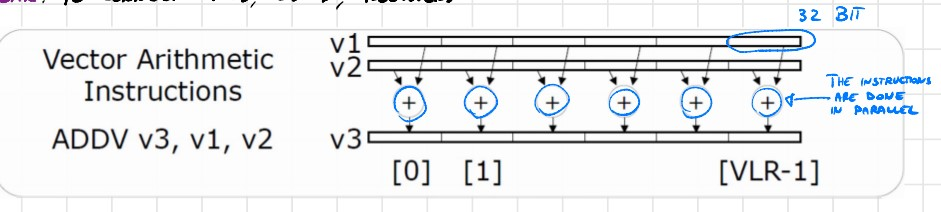
\includegraphics[width=0.5\linewidth]{Images/Screenshot_31.jpg}
    \caption{Arithmetic Instruction}
    \label{fig:enter-label}
\end{figure}
\subsubsection{VMIPS}

The \textit{VMIPS} is an architecture loosely based on \textit{CRAY-1} supercomputer.
It features:

\begin{itemize}
  \item \(8\) \textbf{Vector registers}
        \begin{itemize}
          \item each register holds a \(64\) elements vector with \(64\) bits per element
          \item the register file has at least \(16\) read ports and \(8\) write ports
        \end{itemize}
  \item \textbf{Vector functional units}
        \begin{itemize}
          \item fully pipelined so they can start a new operation every cycle
        \end{itemize}
  \item \textbf{Vector load store unit}
        \begin{itemize}
          \item fully pipelined so they can read one word per clock cycle
        \end{itemize}
  \item \(32\) general-purpose \textbf{scalar registers}
  \item \(32\) floating point \textbf{scalar registers}
  \item Cross-bar to connect FUs, LSUs, and register
\end{itemize}
\clearpage
\begin{figure}[h!]
    \centering
    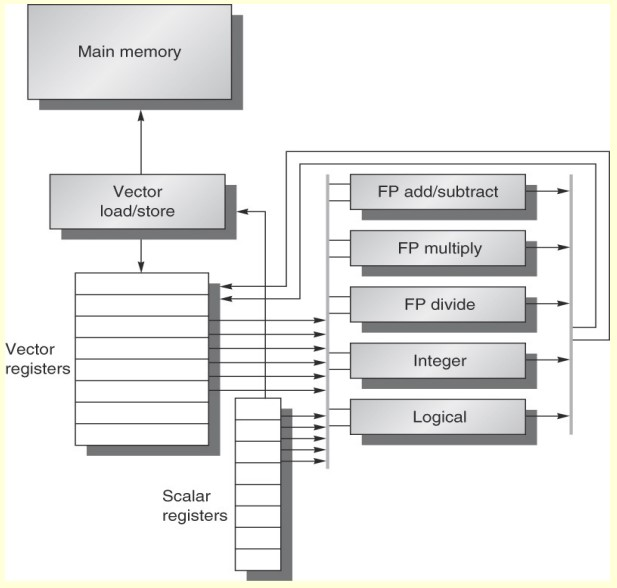
\includegraphics[width=0.5\linewidth]{Images/Screenshot_28.jpg}
    \caption{VMIPS architecture}
    \label{fig:enter-label}
\end{figure}
\subsection{DAXPY Operation}
This operation is from well known type of operation 
\begin{equation*}
    B = a*X+B
\end{equation*}
It's used in ML applications but also in multimedia.\\
\textit{Example of vector code}\footnote{OCIO ALLE LOOP CARRIED}:

\begin{center}
  \bigskip
  \begin{verbatim}
// C code
for (i = 0; i < 64; i++)
  C[i] = A[i] + B[i];
\end{verbatim}
\end{center}

\begin{minipage}[t]{0.495\textwidth}
  \begin{verbatim}
  // Scalar Code
  LI R4, //64
loop:
  L.D F0, 0(R1)
  L.D F2, 0(R2)
  ADD.D F4, F2, F0
  S.D F4, 0(R3)
  DADDIU R1, 8
  DADDIU R2, 8
  DADDIU R3, 8
  DSUBIU R4, 1
  BNEZ R4, loop
\end{verbatim}
\end{minipage}
\begin{minipage}[t]{0.495\textwidth}
  \begin{verbatim}
// Vector Code
LI VLR, //64
LV V1, R1
LV V2, R2
ADDV.D V3,V1,V2
SV V3, R3
  \end{verbatim}
\end{minipage}
In the scalar version, we will have 9 instructions in the loop for 64 elements and 2 initialization instruction
\begin{equation*}
    (64 \cdot 9 ) + 2 = 578\quad instruction\quad per \quad loop
\end{equation*}
In the vectorial version, we have a slightly reduce of instructions, we will have 5 instructions per 64 elements so 
\begin{equation*}
    5\cdot 64 = 321 \quad Clock
\end{equation*}
But this could be better if we put some optimization.
\subsubsection{Vector Execution Time}

\textit{VMIPS} functional units consume one vector element per clock cycle, so the execution time of one vector instruction is approximately the vector length.

To simplify the calculations, the \textbf{Convoy notion} has been introduced:
it considers a set of vector instructions that could potentially execute together \textit{(generating no structural hazards)}:
for a vector of length \(n\) and \(m\) convoys in a program, \(n \cdot m\) clock cycles are needed.
\begin{figure}[h!]
    \centering
    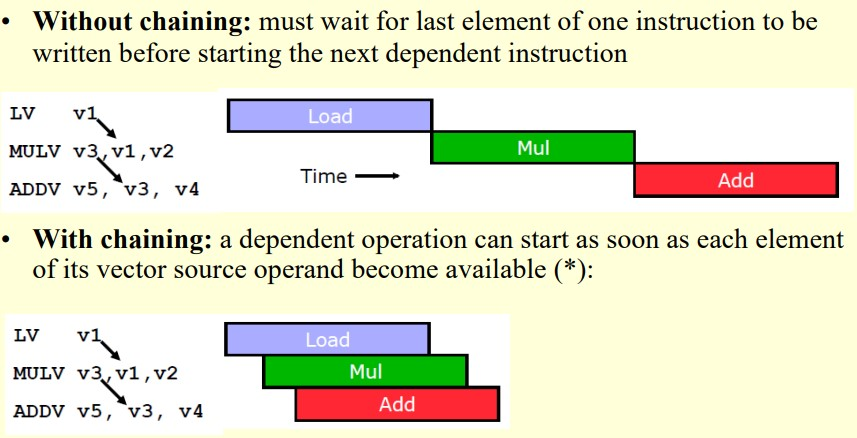
\includegraphics[width=0.5\linewidth]{Images/Screenshot_30.jpg}
    \caption{With or Without Chaining}
    \label{fig:enter-label}
\end{figure}
\\With this optimization, we go from $321$ Clock to $69$ Clock. This optimization will also be safe in terms of data dependency because we start use data when is already solved.
\subsubsection{Advantages over scalar}

\begin{itemize}
  \item \textbf{Vectors operations chaining}
        \begin{itemize}
          \item a vector operation can start as soon as the individual elements of its vector source operand become available
          \item the results of the first functional unit in the chain are forwarded to the second functional unit
          \item implemented by allowing the processor to read and write a particular vector register at the same time provided it is to different scalar elements
          \item flexible chaining: allow a vector instruction to chain to essentially any other vector instruction, assuming that it does not generate any structural hazard
        \end{itemize}
  \item \textbf{Pipeline stalls greatly decreased}
        \begin{itemize}
          \item vector version: only the first element of the vector must be stalled, and after that, the results can come out at every cycle
          \item a scalar processor can try to get a similar effect through loop unrolling but it cannot get the dynamic instruction count to decrease
        \end{itemize}
  \item \textbf{The operations are executed in parallel}, along multiple lines
\end{itemize}
\subsubsection{Multiple Lanes}
Instead of generating an element per clock cycle in one lane, I can spread the elements into multiple lanes to improve the vector performance
\begin{figure}[h!]
    \centering
    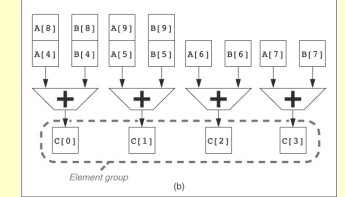
\includegraphics[width=0.25\linewidth]{Images/Screenshot_32.jpg}
    \caption{Multiple Lane}
    \label{fig:enter-label}
\end{figure}
\clearpage
\subsubsection{Vector Lenght Controller}
The Maximum Vector Lenght(\textit{MVL}) is the physical length of the vector register in a machine, but if we have some differences?\\
We can have 2 cases:
\begin{itemize}
    \item Vector smaller,  with the register \textit{Vector-Lenght Register} we can control the length of any vector operation and we can set a smaller value than \textit{MVL}.
    \item Vector Unknown at compile time, we shoud use a technique called \textit{Strip Mining}, to restructure the code in a \textit{\textbf{Remainder}}\footnote{$NmodMVL$} and in different blocks equal to \textit{MVL}.
\begin{figure}[h!]
    \centering
    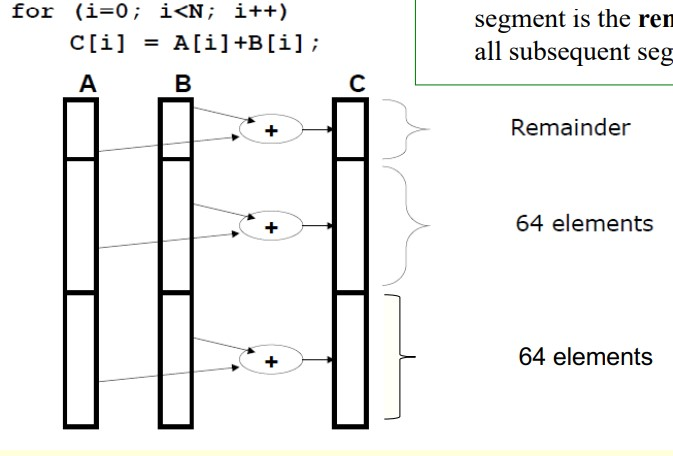
\includegraphics[width=0.5\linewidth]{Images/Screenshot_33.jpg}
    \caption{Strip Mining}
    \label{fig:enter-label}
\end{figure}
\end{itemize}
\subsubsection{Vector Mask Register}
What if there is a control statement in our loop?\\
We can use a \textit{\textbf{Vector Mask Register}}(\textit{VMR}), to "disable" some elements to not perform the operation in the element that does not satisfy those conditions.\\
Every Vector instruction operates \textbf{ONLY} to the vector elements whose corresponding mask is set to 1.
\subsubsection{Stride}
It's called \textbf{the stride} of an array \textit{(also referred to as increment, pitch, or step size)} the number of locations in memory between the beginnings of successive array elements, measured in bytes or units of the size of the array's elements. The stride \textbf{cannot be smaller} than the element size but can be larger, indicating extra space between elements.\\
This idea is used in example when I'm using a matrix and I want to use it by the column and not by the row, so I've to put a load instruction with a stride, to jump into the element I need.
\clearpage
\subsubsection{Scatter and Gatter}
This operation is used in sparse matrix, this type of matrix is very common in ML.\begin{figure}[h!]
    \centering
    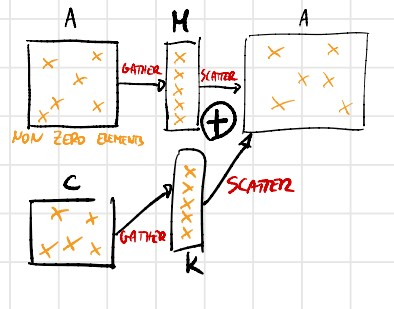
\includegraphics[width=0.5\linewidth]{Screenshot_34.jpg}
    \caption{Scatter and gatter}
    \label{fig:enter-label}
\end{figure}
\clearpage
\section{GPU}
Originally \textit{(in the mid '90s)}, \textit{GPUs} were dedicated fixed functions for generating 3D graphics, including high-performance \textit{(SP)} floating point units.
They provided workstation-like graphics for PCs while the user had no real way to program them, but they could merely configure the pipeline.

Over time, more programmable features were added to the \textit{GPU}, enabling millions of vertices to be rendered in a single frame with very constrained programming models.

Some users noticed they could do general-purpose computation by mapping input and output data to images and computation to vertex and pixel shading computations.
It was however a very difficult programming model as the programmer had to exploit the graphics pipeline to perform general computation.

\subsubsection{General Purpose \textit{GPUs} - \textit{GP-GPUS}}

In \(2006\), \textit{NVIDIA} introduced \textit{GeForce 8800 GPU} supporting a new programming language, called \texttt{CUDA} \textit{("Compute Unified Device Architecture")}.
Subsequently, the other companies in the industry started pushing for \texttt{OpenCL} \textit{("Open Computing Language")}, a vendor-neutral version of the same language available for multiple platforms.

\texttt{CUDA} takes advantage of the \textit{GPU} computational performance and memory bandwidth to accelerate some kernels for general-purpose computing.
The host \textit{CPU} issues data-parallel kernels to \textit{GP-GPU} device for execution.

\bigskip
\texttt{CUDA} programming model:

\begin{itemize}
  \item The \textbf{programmer writes} a serial program that calls parallel \textbf{kernels}
  \item A \textbf{kernel executes} in parallel across a set of parallel \textbf{threads}
  \item The \textbf{programmer organizes} these threads into thread block and grids of \textbf{thread blocks}
  \item A \textbf{thread block} is a set of concurrent threads that can cooperate among themselves through barrier synchronization and shared memory space private to the block
  \item A \textbf{grid} is a set of thread blocks that may be executed independently and thus may execute in parallel \textit{(or any order)}
        \begin{itemize}
          \item thread \textbf{creation}, \textbf{scheduling} and \textbf{termination} are handled by \textbf{underlying hardware}
          \item \texttt{CUDA} model \textbf{virtualizes} the processor
        \end{itemize}
\end{itemize}

\subsubsection{Hardware execution model}

\begin{itemize}
  \item The \textit{GPU} is built from \textbf{multiple parallel cores}, each one containing a multithreaded \textit{SIMD} processor with multiple lanes but without scalar processor
        \begin{itemize}
          \item each tread block executes on \textbf{one core}
          \item some newer models feature a \textbf{scalar unit}
        \end{itemize}
  \item The \textit{CPU} \textbf{sends the whole grid over to the} \textit{GPU}, which distributes thread blocks among cores
        \begin{itemize}
          \item the programmer is \textbf{not aware} of the number of cores
        \end{itemize}
\end{itemize}

\bigskip
GPUs use a \textbf{SIMT} \textit{(Single Instruction Multiple Thread)} model, where individual \textit{(scalar)} instruction streams for each \texttt{CUDA} thread are grouped for \textit{SIMD} execution on the hardware.
\textit{NVIDIA} groups \(32\) threads (\(\mu T\)) into a \textbf{warp}.

Warps are multithreaded on cores, and each of them is managed by the hardware:
one warp composed by \(32\) threads \textit{\(\mu T\)} represents a single thread in the hardware.
Multiple threads are then interleaved in execution on a single core to reduce latencies to memory and FUs.

A single thread block can contain multiple warps \textit{(up to \(512 \mu T\) in \texttt{CUDA})}, all mapped into a single core;
multiple blocks can also execute on a single core.
Individual parallel threads of a warp start together but are free to branch and execute in \textbf{parallel}.

\textit{SIMT} model gives the illusion of many independent threads running on a single core, but for efficiency's sake, the programmer must try and keep each \(\mu T\) as aligned as possible, in \textit{SIMD} fashion.

\bigskip
Simple \texttt{if-then-else} instructions are compiled into predicated execution, equivalent to vector masking ;
more complex control flow code must be compiled into branches.

Hardware tracks which \(\mu T\) take or don't take branches:
if all go in the same direction, the hardware can execute the block in \textit{SIMD} fashion;
otherwise, a mask vector indicating \textit{taken} or \textit{not taken} is created.

The \textit{not taken} paths keep running under the mask, while the \textit{taken} paths \texttt{PC} and mask are pushed into a hardware stack to be executed later.

\bigskip
An illustration of the hardware execution model is shown in Figure~\ref{fig:gpu-hardware-model}.

\begin{figure}[htbp]
  \bigskip
  \centering
  \tikzfig[1]{image-67.tikz}
  \caption{Hardware execution model}
  \label{fig:gpu-hardware-model}
  \bigskip
\end{figure}



\end{document}



